% GENERAL INFORMATION: HardwareX is an open access journal established to promote free and open source designing, building and customizing of scientific infrastructure (hardware). For more details on best practices for sharing open hardware see http://www.oshwa.org/sharing-best-practices/

\documentclass[11pt, letterpaper]{article}
\usepackage[utf8]{inputenc}
\usepackage[margin=1in]{geometry}
\usepackage{titlesec}
\usepackage{tabu}
\usepackage{enumitem}
\usepackage{amssymb}
\usepackage{graphicx}
\usepackage{float}
\newlist{selectlist}{itemize}{2}
\setlist[selectlist]{label=$\square$,leftmargin=*,noitemsep,topsep=0pt}

\usepackage{hyperref}
\hypersetup{
    colorlinks=true,
    linkcolor=blue,
    filecolor=magenta,
    urlcolor=cyan,
}

\usepackage[backend=biber]{biblatex}
\addbibresource{VentMon.bib}

\urlstyle{same}

% Set up the section label formatting
\titleformat{\section}[block]{\hspace{1em}\bfseries}{\thesection.}{0.5em}{}
\titleformat{\subsection}[block]{\hspace{1em}}{\thesubsection}{0.5em}{}

\begin{document}
% Create the title block
\begin{flushleft}

% Remove all text in italics when filling out the template and replace with your manuscripts corresponding text in regular font.

\setlength{\parindent}{0pt}
\setlength{\parskip}{10pt}
% \textbf{\large HardwareX article template}

%Insert title
%Max. 20 words. A good title should contain the fewest possible words that adequately describe the content of a paper.
\textbf{Title:} VentMon: An Open Source Inline Ventilator Tester and Monitor

%Insert Authors
\textbf{Authors:} Robert L. Read, Lauria Clarke, Geoff Mulligan

%Insert Affiliations
\textbf{Affiliations:} Public Invention with support from the \textit{Protocol Labs} and the \textit{Mozilla Foundation}

%Insert Contact Email
%Include institutional email address of the corresponding author
\textbf{Contact email:} read.robert@gmail.com

%Insert Abstract
%Max. 200 words. Remember that the abstract is what readers see first in electronic abstracting and indexing services. This is the advertisement of your article. Make it interesting, and easy to be understood. Be accurate and specific, keep it as brief as possible.
\textbf{Abstract:}

Humanitarian engineers responded to the pandemic ventilator shortage of March, 2020
by beginning over 100 open source ventilator projects\cite{COVID19VENTLIST,pearce2020review}.
By {\em ventilator}, we mean both an invasive ventilator (requiring intubation of the patient) and non-invasive ventilator (generally supporting spontaneously breathing).
Inexpensive ventilator test equipment can facilitate projects forced to be geographically distributed by lockdowns.
The VentMon is a modular, open source, IoT-enabled tester that plugs into a standard 22mm airway between a ventilator and a physical test lung to test any ventilator.
The VentMon measures flow, pressure, fractional oxygen, humidity, and temperature.
Data is stored and graphed at a data lake accessible to all devlopment team members, and, eventually, clinicians.
The open source design of the VentMon,
its firmware, and cloud-based software may allow it to be used as a component of modular ventilators to provide a clinical readout.
The software system surrounding VentMon has been designed to be as modular and composable as possible.
By combining new, openly published standards for data with composable and modifiable hardware,
the VentMon forms the beginning of an open system or eco-system of ventilation devices and data.
Thanks to grants, 20 VentMons have been given away free of charge to pandemic response teams building open source ventilators.


%Insert Keywords
% At least 3 keywords. There is no limit on the no. of keywords you can list. Please remember that effective keywords should not repeat words appearing in your title, and should be neither too general nor too narrow.
\textbf{Keywords:} COVID-19, open source medical device, ventilator, pandemic response, IoT, respiration waveform

\newpage
\textbf{Specifications table:}

\tabulinesep=1ex
\begin{tabu} to \linewidth {|X|X[3,l]|}
\hline  \textbf{Hardware name} &
  %Please specify the name of the hardware that you invented / customized
  VentMon
  \\
  \hline \textbf{Subject area} & %
  % Please state the subject area most relevant to the original community for which this hardware was developed. Example subject areas are listed below
 Educational Tools and Open Source Alternatives to Existing Infrastructure
  \\
  \hline \textbf{Hardware type} &
Field measurements and sensors,
Electrical engineering and computer science
  \\
\hline \textbf{Open source license} &
  %Please specify the open source license. For more details see the guide to authors.
 MIT License, CERN-OHL-S
  \\
\hline \textbf{Cost of hardware} &
  %Approximate cost of hardware (complete breakdown will be included in the Bill of Materials).
\$280
  \\
  \hline \textbf{Source file repository} &

  VentMon: \linebreak
  \href{https://doi.org/10.5281/zenodo.4079170}{https://doi.org/10.5281/zenodo.4079170}
  \linebreak
  PIRDS (Public Invention Respiration Data Standard): \linebreak
  \href{http://doi.org/10.5281/zenodo.4079377}{http://doi.org/10.5281/zenodo.4079377}
  \linebreak
  PIRDS logger: \linebreak
  \href{Zenodo. http://doi.org/10.5281/zenodo.4079382}{Zenodo. http://doi.org/10.5281/zenodo.4079382}
  \linebreak
  SFM3X00: \linebreak
  \href{http://doi.org/10.5281/zenodo.4079355}{http://doi.org/10.5281/zenodo.4079355} \linebreak
  VentDisplay: \linebreak
  \href{http://doi.org/10.5281/zenodo.4079374}{http://doi.org/10.5281/zenodo.4079374} \linebreak
  \linebreak

  % Link to the source file repository
      % insert a DOI URL to an approved source file repository:  Mendeley Data, theOSF, or Zenodo (instructions).  For example: "https://doi.org/10.5281/zenodo.3346799"
      % If there is no external repository write “Available in the article”
  %% \textit{DOI URL to an approved source file repository:  \href{https://data.mendeley.com/}{Mendeley Data}, the \href{http://osf.io}{OSF}, or \href{https://zenodo.org/}{Zenodo} \href{https://doi.org/10.5281/zenodo.3346799}{(instructions)}. For example:} \textit{https://doi.org/10.5281/zenodo.3346799}
%  \linebreak
%  \linebreak
\\\hline
\end{tabu}
\end{flushleft}
% create the main body of the paper

\section{Hardware in context}
% Include a short description of the hardware, putting into context of similar open hardware and proprietary equipment in the field.
The Coronavirus pandemic has created a potential global shortage of ventilators\cite{pearce2020review}, which has abated in the wealthy nations.
Ventilators are expensive to manufacture and during uncertain times supply chains can be disrupted, increasing the cost and scarcity of these devices. Since the beginning of the pandemic in March,
there has been a large movement to develop cheaper,
more supply chain-resilient ventilators.
The urgency and goals of this movement have shifted as the global understanding of the virus has evolved. Regardless of the current state of this movement, however, the use of
open source medical devices in resource-limited emergency situations---common during a global pandemic---is a topic that has come to the forefront of may conversations about preparedness and treatment.
Medical devices require rigorous testing before they can be used on the general public.
Open source medical devices require the same level, if not more, scrutiny and documentation. If an open source movement is to succeed in this field, the tools to test and validate medical
devices must be accessible.
The goal of VentMon is to provide an equally open source, community based verification solution to increase the efficiency and accuracy of the development process for socially distanced,
potentially international teams making open source ventilator, Bilevel Positive Airway Pressure (BPAP), and Powered Air-Purifying Respirator (PAPR) devices.

\section{Hardware description}
% Describe the hardware, highlighting the customization rather than the steps of the procedure. Highlight how it differs/which advantage it offers over pre-existing methods. For example, how could this hardware: be compared to other hardware in terms of cost or ease of use, be used in the development of further designs in a particular area, and so on.

% > Add 3-5 bulleted points to broadly explain to other researchers how the hardware could be potentially useful to them, for either standard or novel laboratory tasks, inside or outside of the original user community.

The VentMon plugs directly into a standard 22mm adult airway. As air or medical gases pass through the VentMon, it records flow and pressure, temperature, humidity, and fractional O$_2$ at rates of 25 Hz to once per minute depending on the measurement. When placed in the breathing circuit between a ventilator under test and physical test lung, this data is sent to a public data lake \cite{VentDisplay} using a clearly defined respiration standard \cite{PIRDS}. This data can be graphically rendered either live or statically to provide a display that is typical of the clinical display of advanced ventilators. This functionality is similar to that of commercially available test lung devices, which tend to start at USD\$10,000.

Teams building open pandemic ventilators tend to be poorly funded and geographically distributed. VentMon's connectivity and overall cost address these two challenges by enabling team members on different continents to view waveforms in real time and communicate the necessary adjustments to the ventilator device under test. While reliance on the internet is a strength for a distributed and virtually connected engineering team, it would be an addressable disadvantage in a field hospital.

Being completely open, VentMon supports modification, extension, and has potential for integration into a complete ventilator. A team working to build a ventilator device with a graphical trace of pressure and flow---generally demanded by clinicians for all but emergency transport situations---could incorporate the open source VentMon into its complete design. VentMon has potential to be safe enough and reliable to be used as a monitor on human patients, however it requires much improvement before it is ready for that use.
\\

The VentMon thus offers the following benefits to teams developing ventilation devices. It:
\begin{itemize}
\item is inexpensive,
\item is completely open source and part of a modular hardware/software system that can be customized and extended,
\item allows remote collaboration, and
\item currently provides many of the clinically significant metrics found in commercially available ventilators.
\end{itemize}

\section{Design files}
% The  complete  design  files  must  be  either  uploaded  to  an  approved  online  repository,  uploaded  at the  time  of  submission  on  the  online  Editorial  Manager  submission  interface  as  supplementary materials [CAD files, videos,. . . ], or included in the body of the manuscript [e.g.  figures].  The three approved  online  repositories  are  Mendeley  Data,  the  Open  Science  Framework,  and  Zenodo. See repository instructions: https://doi.org/10.5281/zenodo.3346799

\subsection{Design Files Summary}
% Please include a summary of all design files for your hardware by filling rows of the table below

\tabulinesep=1ex
\begin{tabu} to \linewidth {|X[1.5]|X|X[1.5,1]|X[3]|}
\hline
\textbf{Design filename} & \textbf{File type} & \textbf{Open source license} & \textbf{Location of the file} \\\hline
%Insert design files
(1) Embedded Firmware (v0.3 PCB version) & C++ Source Code & MIT License &  \href{https://doi.org/10.5281/zenodo.4079170}{10.5281/zenodo.4079170}\\\hline
(2) Embedded Firmware (v0.2 COTS version) & C++ Source Code & MIT License &  \href{https://doi.org/10.5281/zenodo.4291147}{10.5281/zenodo.4291147}\\\hline
(3) VentDisplay PIRDS Data Viewer  & HTML Source Code &  MIT License &  \href{http://doi.org/10.5281/zenodo.4079355}{10.5281/zenodo.4079374} \\\hline
(4) PIRDS Data Logger & C Source Files & MIT License & \href{https://doi.org/10.5281/zenodo.4079382}{10.5281/zenodo.4079382} \\\hline
(5) PIRDS Data Standard & Documented standard, and C-language binding & Creative Commons Zero (Universal) for documents, GPL 3.0 for code binding &
\href{http://doi.org/10.5281/zenodo.4079355}{10.5281/zenodo.4079355} \\\hline
(6) VentMon v0.3T PCB & PCB Design Files & MIT License &  \href{https://doi.org/10.5281/zenodo.4079170}{10.5281/zenodo.4079170} (see {\em design/pcb}) \\\hline
(7) Pressure Sensor and Airway Adaptor & STL File & MIT License &  \href{https://doi.org/10.5281/zenodo.4079170}{10.5281/zenodo.4079170} (see {\em design/3dparts}) \\\hline

% Design file 3 & File type & License & Link \\\hline

\end{tabu}
\vspace{0.5cm}

We promote an open, modular, and composable respiration ecosystem. Therefore, we have more separate repositories and modules than would strictly be needed if we were only making the VentMon project. Our hope is that smaller modules may be reusable by others who do not need the VentMon specifically, but may have need for a particular component.

\begin{enumerate}
\item The main firmware is written in the Arduino environment. The firmware targets an ESP32, but could easily apply to other boards. This core firmware manages reading the various sensors, and outputs its data both on its small built-in OLED (used for functional testing), and via the PIRDS standard to a public data lake where a separate module renders it in a graphical display appropriate for a clinician.
\item Our current focus is on a printed circuit board version of the VentMon\cite{ventmonpcb}. However, we also report here a system that can be made by an amateur using only commercial off-the-shelf (COTS) parts---version T0.2. Software that matches this version it is tagged as such.
\item VentMon has a tiny OLED screen which is used to graph pressure for quick ``smoke'' testing. For serious performance testing and eventual clinical use, we use VentDisplay, a browser-delivered JavaScript code that presents a full clinical display.
\item The VentDisplay software can be pointed at any data logger that serves up data in the PIRDS format. This logger takes data from UDP packets and writes them to a file, which can then be served up by a webserver to any requester.
\item Integral to the VentDisplay and PIRDS Data Logger is the Public Invention Respiration Data Standard (PIRDS). This is a documented standard.
\item The VentMon v0.3T printed circuit board is designed with EAGLE CAD.
\item A small 3D printed housing epoxied over the ambient air quality sensor with a tiny pressure port allows us to share the air with the main pressure hose.
\end{enumerate}


% For each design file listed in the summary above, include a short description of the file below (one or two sentences)

\section{Bill of materials}

% For a complex Bill of Materials, the complete Bill of Materials (editable spreadsheet file e.g., ODS file type or PDF file) can be uploaded in an open access online location such as the Open Science Frameworks repository. Include the link here. Alternatively, the Bill of Materials can be uploaded at the time of submission on the online Elsevier submission interface as supplementary material.

% > To make it easy to tell which item in the Bill of Materials corresponds to which component in your design file(s), use matching designators in both places, or otherwise explain the correspondence.

% > For material type, select from: Metal, semi-conductor, ceramic, polymer, biomaterial, organic, inorganic, composite, nanomaterial, semiconductor, non-specific, or other

The Bill of Materials specifies the parts needed to build the VentMon in a simple enclosure with drilled-out ports for cables.
The parts are typical of hobby electronics.

\tabulinesep=1ex
\begin{tabu} to \linewidth {|X[0.5]|X[3]|X[0.5]|X|X|X|X[3]|}
  \hline
\textbf{ Designator} &	\textbf{Component} & \textbf{Number} & \textbf{Cost/Unit} & \textbf{Total Cost}& \textbf{Source} & \textbf{Material Type} \\\hline
U1 &	PARTICLE ETHERNET FEATHERWING &	1 &	\$20.11 &	\$20.11  &	Adafruit &	Semiconductor/Other \\\hline
U2 &	HUZZAH32 ESP32 FEATHER MALE HDR	& 1 &	\$21.95	& \$21.95 &	Adafruit&	Semiconductor/Other \\\hline
U3 &	SPARKFUN QWIIC SHIELD FOR THING	& 1 &	\$3.50	& \$3.50 &	Digikey	& Semiconductor/Other \\\hline
U4 &	ADS1115 16 Bit ADC &	1&	\$14.95	& \$14.95 &	Adafruit	& Semiconductor/Other \\\hline
U5 &	OLED Feather Wing &	1&	\$14.95	& \$14.95 &	Adafruit &	Semiconductor/Other \\\hline
C1, C2 &	QWIIC CABLE - 200MM &	2 &	\$1.56 &	\$3.12 &	Digikey	& Metal/Plastic \\\hline
C3 &	USB Cable &	1 &	\$1.80 &	\$1.80	& Digikey &	Metal/Plastic \\\hline
C4 &	Oxygen Sensor Cable &	1 &	\$4.00 &	\$4.00 &	Oxycheq &	Metal/Plastic \\\hline
H1 &	M2.5 Screws &	12 &	\$0.38	& \$4.56 &	Digikey	& Metal \\\hline
H2 &	M2.5 Standoffs - Female, Female	& 6 &	\$0.45 &	\$2.70	& Digikey &	Metal \\\hline
OS1 &	R-17S Oxygen Sensor &	1 &	\$80.00 &	\$80.00	 & Oxycheq &	Metal/Plastic \\\hline
FS1 &	\textbf{Flow Sensor} &	1 & \textbf{see note below}	&	\$0.00	& &	Metal/Plastic \\\hline
PS1, PS2 &	BME680 SENSOR EVAL BOARD &	2 &	\$22.50 &	\$45.00	& Adafruit &	Semiconductor/Other \\\hline
P1 &	Processor Enclosure &	1 &	\$9.95 &	\$9.95 &	Digikey	 & Plastic \\\hline
P2 &	Bleed Adaptor	& 1 &	\$5.50 &	\$5.50 &	Oxygen Supply	& Plastic \\\hline
P3 &	Oxygen Sensor T	& 1 &	\$9.00 &	\$9.00	& Oxycheq &	Plastic \\\hline
P4 &	15 mm OD to 22 mm OD adaptor &	1 &	\$0.54 & 	\$0.54	& &	Plastic \\\hline
P5 &	15 mm ID to 22 mm OD adaptor &	1 &	\$0.35 & 	\$0.35	& &	Plastic \\\hline
T1 &	Oxygen Tubing &	1 &	\$2.25	& \$2.25 &	Oxygen Supply	& Plastic \\\hline
\end{tabu}

Note: The flow sensor is one of the most expensive and critical parts. Throughout mid-2020 there was a global shortage of flow sensors, including the four electrically compatible with the VentMon as currently designed. The Sensirion SFM3400-AW (\$180US) (a neonatal version with limited maximum flow sensing), SFM3200-33-D (disposable version \$40USD), Sensirion SFM3200-250 (\$145USD), and Sensirion SFM3200-AW (\$180USD autoclavable version). We shipped VentMons with all of these depending on availability. The VentMon is not currently designed for use with humans, but if it were, the autoclavable version would have the advantage of sanitizability if a complete sanitization procedure were designed. This is important, as we hope the VentMon will be modified and integrated into a rapidly manufactured ventilator, for which sanitization is critical.


The link below is to a spreadsheet which is includes the PCB-version, which is very similar except for the PCB itself. By following this link: \href{https://doi.org/10.5281/zenodo.4289426}{VentMon  BOM}, you can reach browsable URLs to most of the non-commodity parts. The specific BOM for the SMD parts needed to assemble the PCB can be found in our GitHub repo in the directory named {\em design/pcb}  along with the Eagle files: \cite{ventmonpcb}.


\section{Build instructions}
%Provide detailed, step by step instructions for the construction of the reported hardware include all necessary information for reproducing the submitted hardware.
% > Explain and, when possible, characterize design decisions. Including design alternatives if they exist.
% > Use visual instructions such as schematics, images, and videos.
% > Clearly reference design files and component parts described in the Design File Summary and Bill of Materials.
% >Highlight potential safety concerns that may arise

Two versions of VentMon can be assembled depending on availability of parts and time. The most physically robust and complete version of VentMon requires the purchase and manufacture of a PCB as well as a number of 3D printed plastic parts. This version of the device requires the least amount of time to assemble and contains fewest discrete components. The designs of the PCB and 3D printed parts are fully open. Due to the relatively high single-unit cost of PCB manufacture and assembly it makes most sense to use the PCB if you are building 10 or more VentMons. VentMon can also be created using off the shelf components readily available from DIY electronics suppliers. This version requires significantly more assembly time. We believe this has been done twice by third parties with little to no assistance from the VentMon team. Both assembly procedures are outlined below.

\subsection{COTS Based VentMon (v0.2T)}

{\em The VentMon v0.2T is not meant to be used on human patients. }
The COTS version uses firmware v0.2 tagged as such\cite{VentMon02}. This version is somewhat incompatible
with v0.3 (described below), which uses a PCB, and which is
the focus of our main development.

\begin{enumerate}

%-----------------------------------------------------------
% QWIIC SHIELD
\item
Qwiic Shield Assembly

See Figure \ref{fig:qwiic} on page \pageref{fig:qwiic} for final assembly of Qwiic Shield.

\begin{enumerate}[label=1.\arabic*]
\item
Trim two pieces of male header pins that are two positions long and one piece that is four positions long.
\item
With the connector side of the board facing up, solder one of the two position headers into the two holes labeled SDA and SCL.
\item
Solder the other two position header into the last two holes on the row along the opposite side.
\item
Solder the four position header into the last four holes along the right side. This should provide connections to the GND and 3V3 through holes.
\item
Connect both sides of the solder bridge to engage the pull-up resistors for the I\textsuperscript{2}C bus.
\end{enumerate}

\begin{figure}[H]
\centering
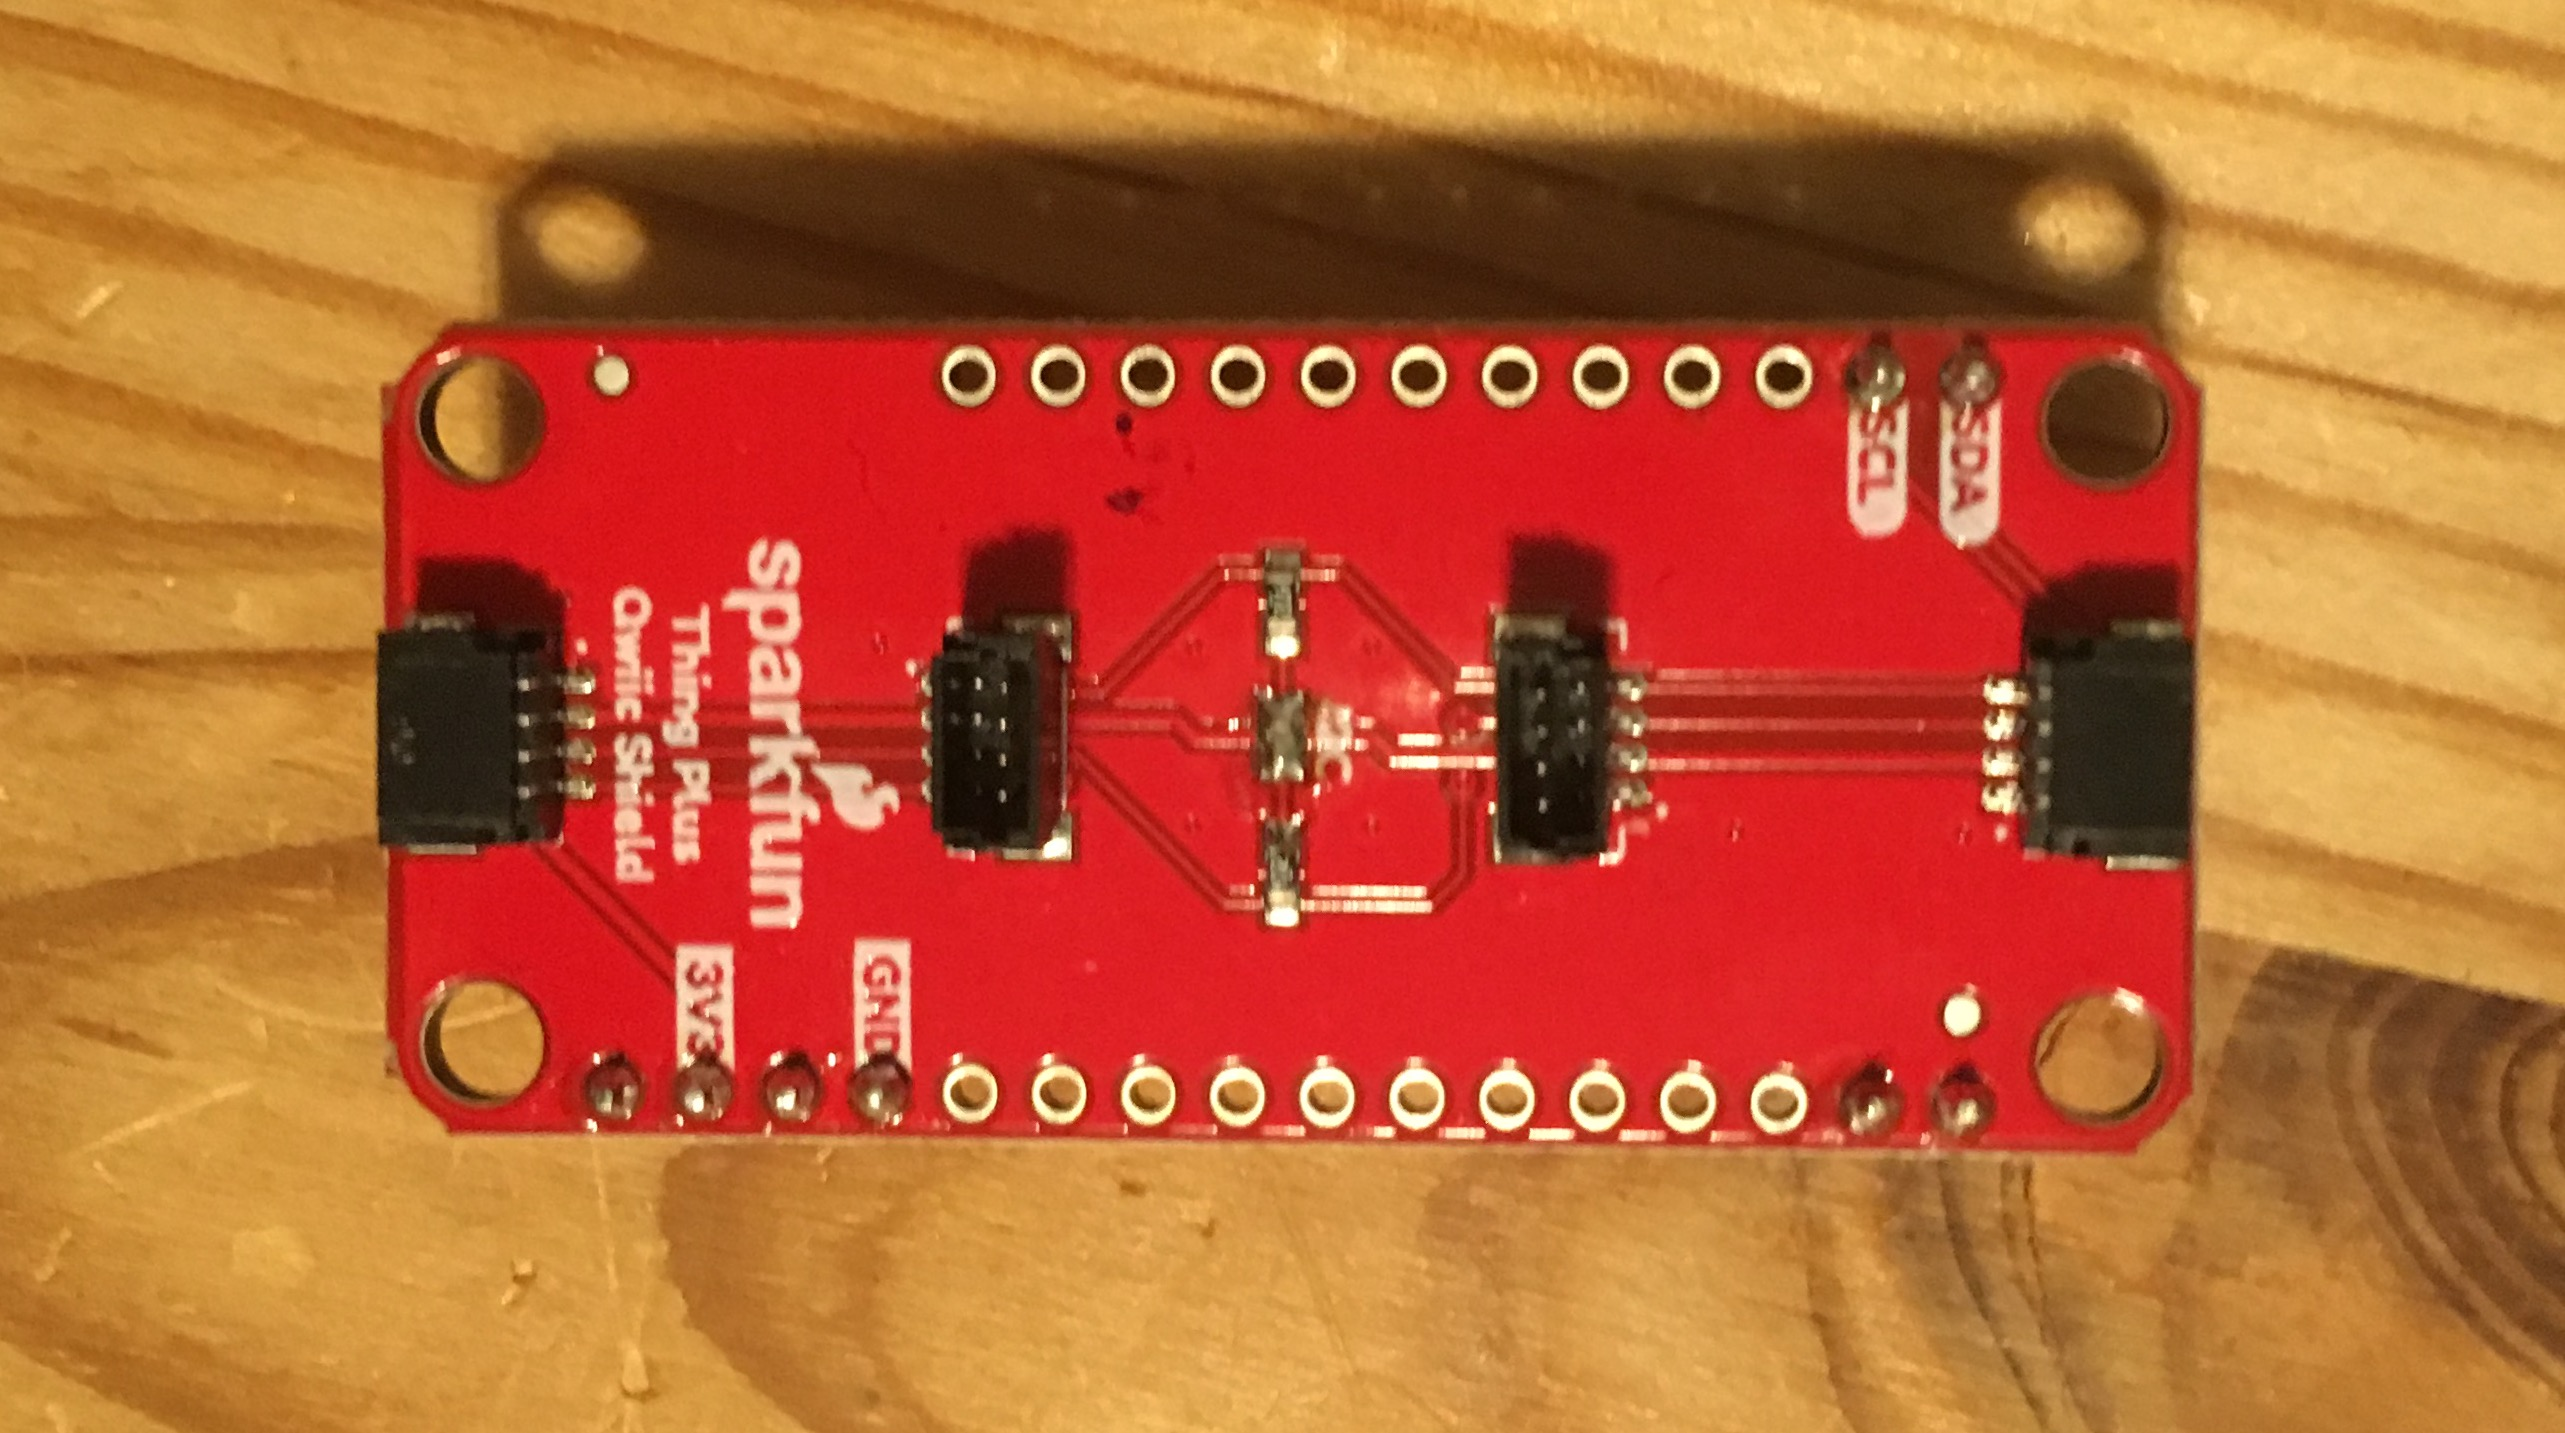
\includegraphics[width=0.45\textwidth]{images/qwiic_top.JPG}
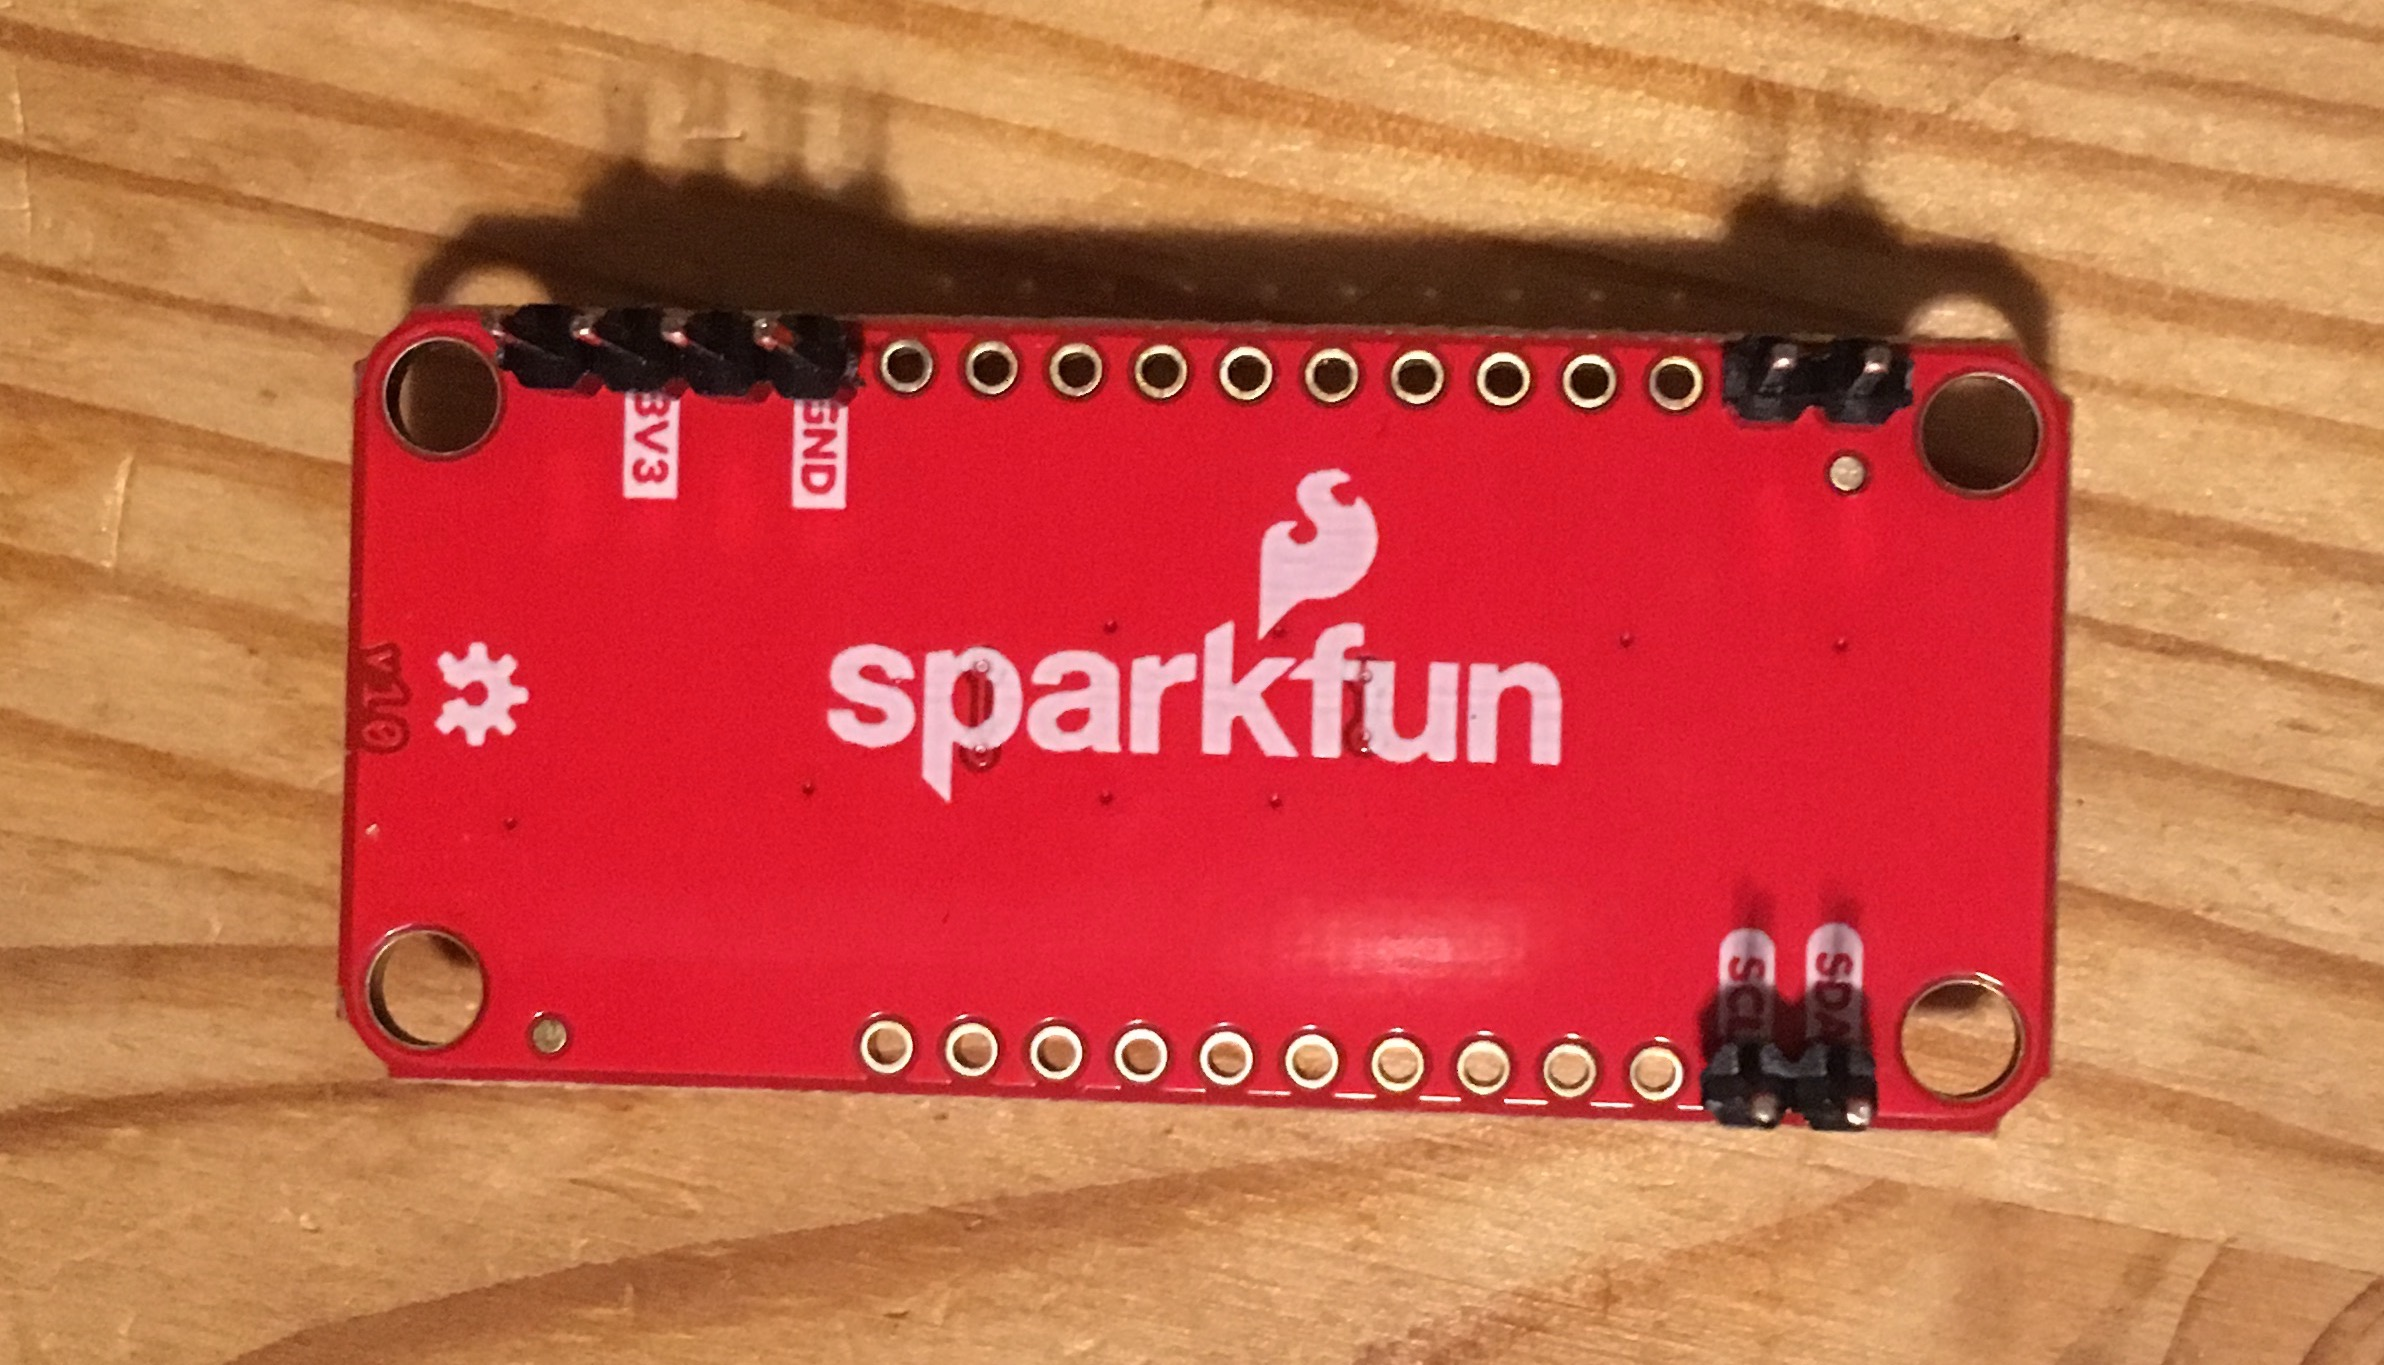
\includegraphics[width=0.44\textwidth]{images/qwiic_bottom.JPG}
\caption{SparkFun Qwiic Shield with male headers and I\textsuperscript{2}C pull-ups connected}
\label{fig:qwiic}
\end{figure}

%-----------------------------------------------------------
% ENCLOSURE
\item \label{itm:enclosure}
Enclosure

Before starting this step download and print the \href{https://github.com/PubInv/ventmon-ventilator-inline-test-monitor/blob/master/design/templates/bottomDrill03.pdf}{drill template}.

\begin{enumerate}[label=2.\arabic*]
\item
Cut out the template and tape it to the enclosure.
\item
Make sure the lid of the enclosure is firmly screwed on before drilling
\item
Drill holes in the locations denoted on template using the recommended drill sizes for each hole.
\end{enumerate}

%-----------------------------------------------------------
% PRESSURE SENSOR
\item
Pressure Sensor Assembly
\begin{enumerate}[label=3.\arabic*]
\item
Drill out mounting holes refer to figure \ref{fig:bme_1} on page \pageref{fig:bme_1}
\begin{enumerate}[label=3.1.\arabic*]
\item
Using the 7/64'' drill bit, carefully enlarge the mounting holes in each corner of the sensor
\item
You can do all four or just two - one on the left side of one board and one on the right side of the other
\end{enumerate}
\item
Cut trace from SDO through hole to sensor. Refer to figure \ref{fig:bme_1} on page \pageref{fig:bme_1}.
\begin{enumerate}[label=3.2.\arabic*]
\item
Carefully cut the trace coming from the SDO hole on the back side of one board
\item
This board will be used to measure the pressure in the breathing circuit
\end{enumerate}
\begin{figure}[H]
\label{fig:bme_1}
\centering
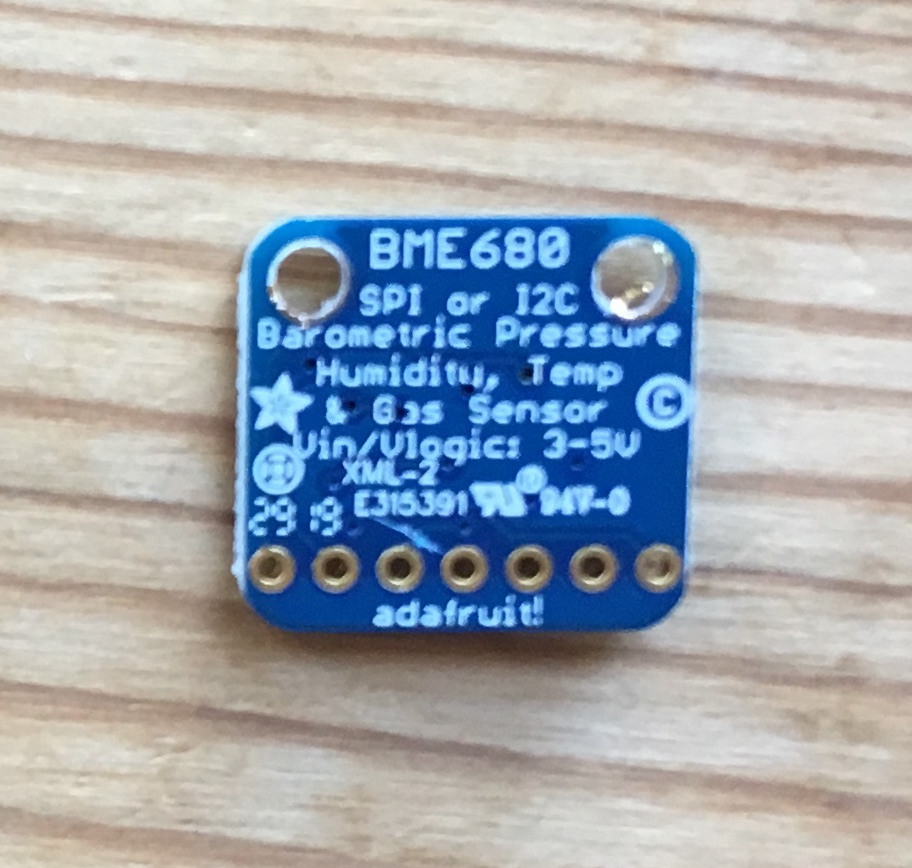
\includegraphics[width=0.45\textwidth]{images/bme_1.JPG}
\caption{BME 280 Eval board with drilled out holes and trace cut}
\end{figure}

\item
Assemble Cable. Refer to figure \ref{fig:bme_qwiic_cable} on page \pageref{fig:bme_qwiic_cable}.
\begin{enumerate}[label=3.3.\arabic*]
\item
Cut one connector off the Qwiic cable
\item
Strip and tin the last $1/4$" of the leads
\end{enumerate}
\begin{figure}[H]
\centering
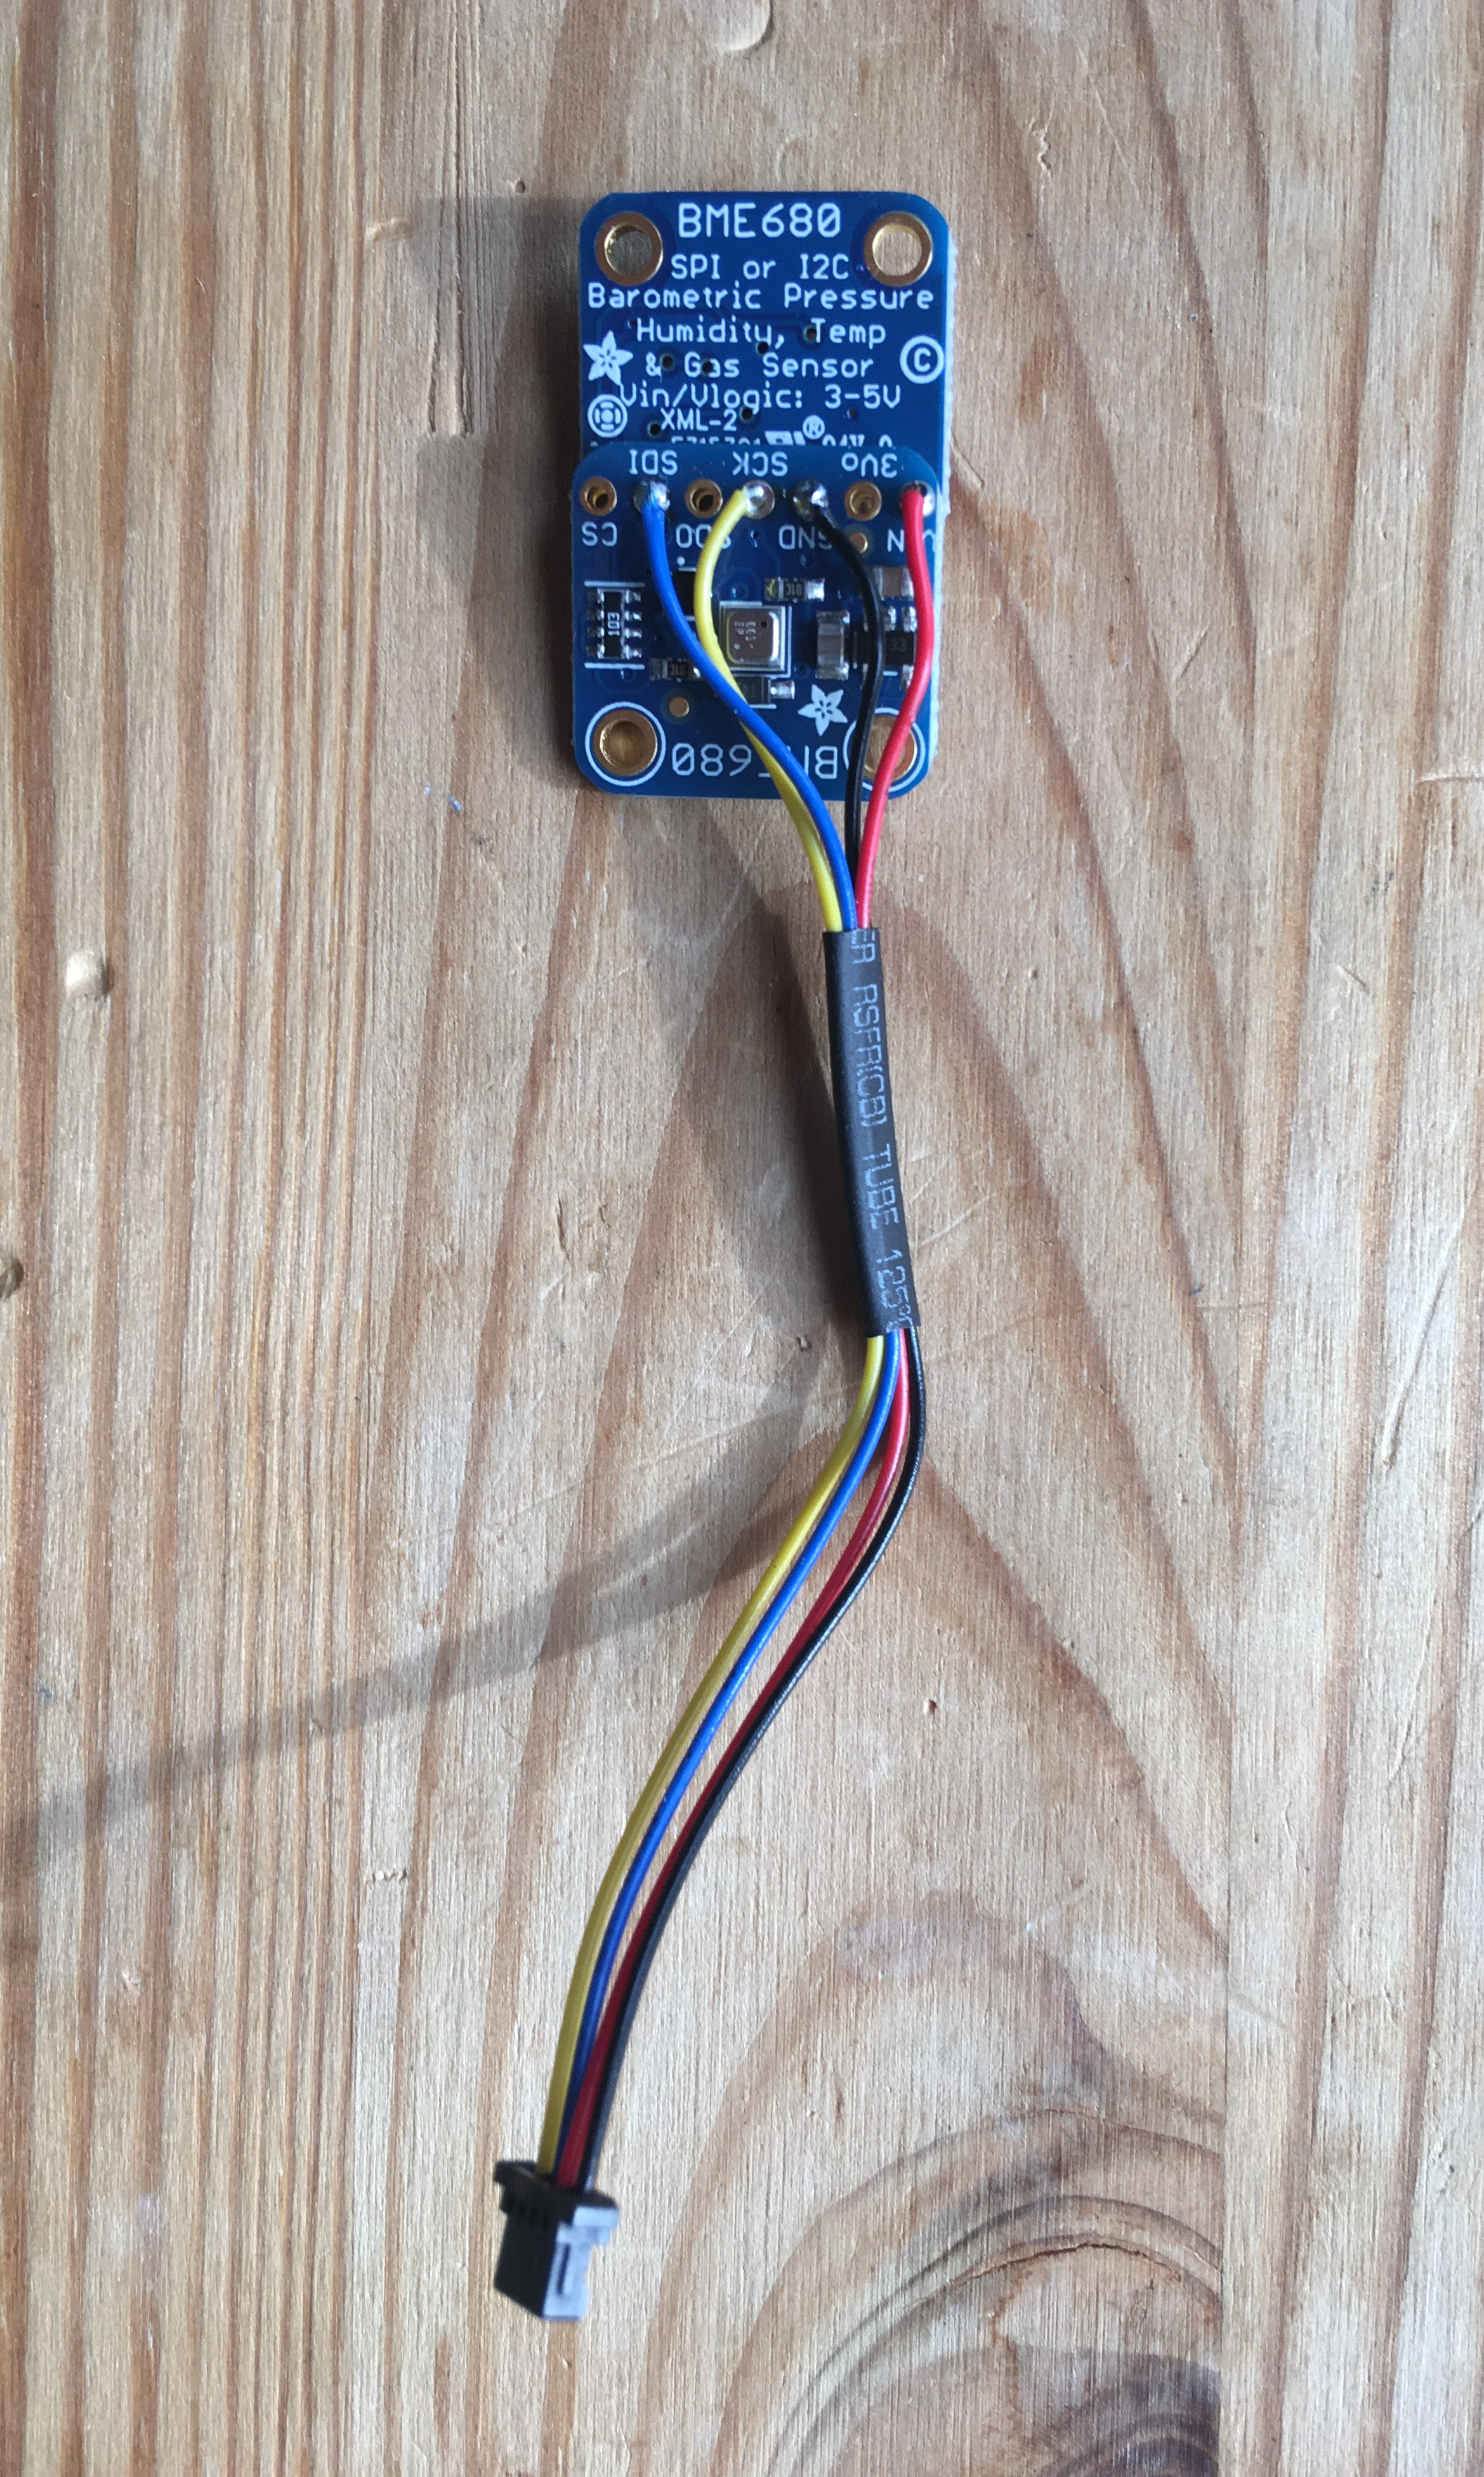
\includegraphics[width=0.5\textwidth]{images/bme_qwiic_cable.JPG}
\caption{Prepared Qwiic cable for BME sensor assembly}
\label{fig:bme_qwiic_cable}
\end{figure}
\item
Connect Sensors to Cable. Refer to figure \ref{fig:bme_and_qwiic_cable} on page \pageref{fig:bme_and_qwiic_cable} and table \ref{tab:pressure} on page \pageref{tab:pressure} for electrical connection.
\begin{enumerate}[label=3.4.\arabic*]
\item
Stack the two sensors on the breadboard and use two paper clips to anchor them
\item
Be sure the board with the cut trace is facing down
\item
Starting with Vin or GND insert the tinned lead through the appropriate hole and apply solder
\item
Flip the sensor assembly over and make sure solder has flowed through both through holes, adding some if needed
\item
Don't worry if the solder does not flow perfectly
\item
Pin the assembly back down and move to another connection following the connection table below
\item
Repeat the steps above until the two boards have been secured and all leads are connected
\item
Re-flow all the joints to ensure a good connection
\end{enumerate}

\begin{table}[H]
\centering
\begin{tabular}{| c | c |}
\hline
Signal & Qwiic Color\\  \hline
GND & black  \\  \hline
VIN & red \\  \hline
SDA & blue \\  \hline
SCL & yellow \\
\hline
\end{tabular}
\caption{pressure sensor wiring}
\label{tab:pressure}
\end{table}

\begin{figure}[H]
\label{fig:bme_and_qwiic_cable}
\centering
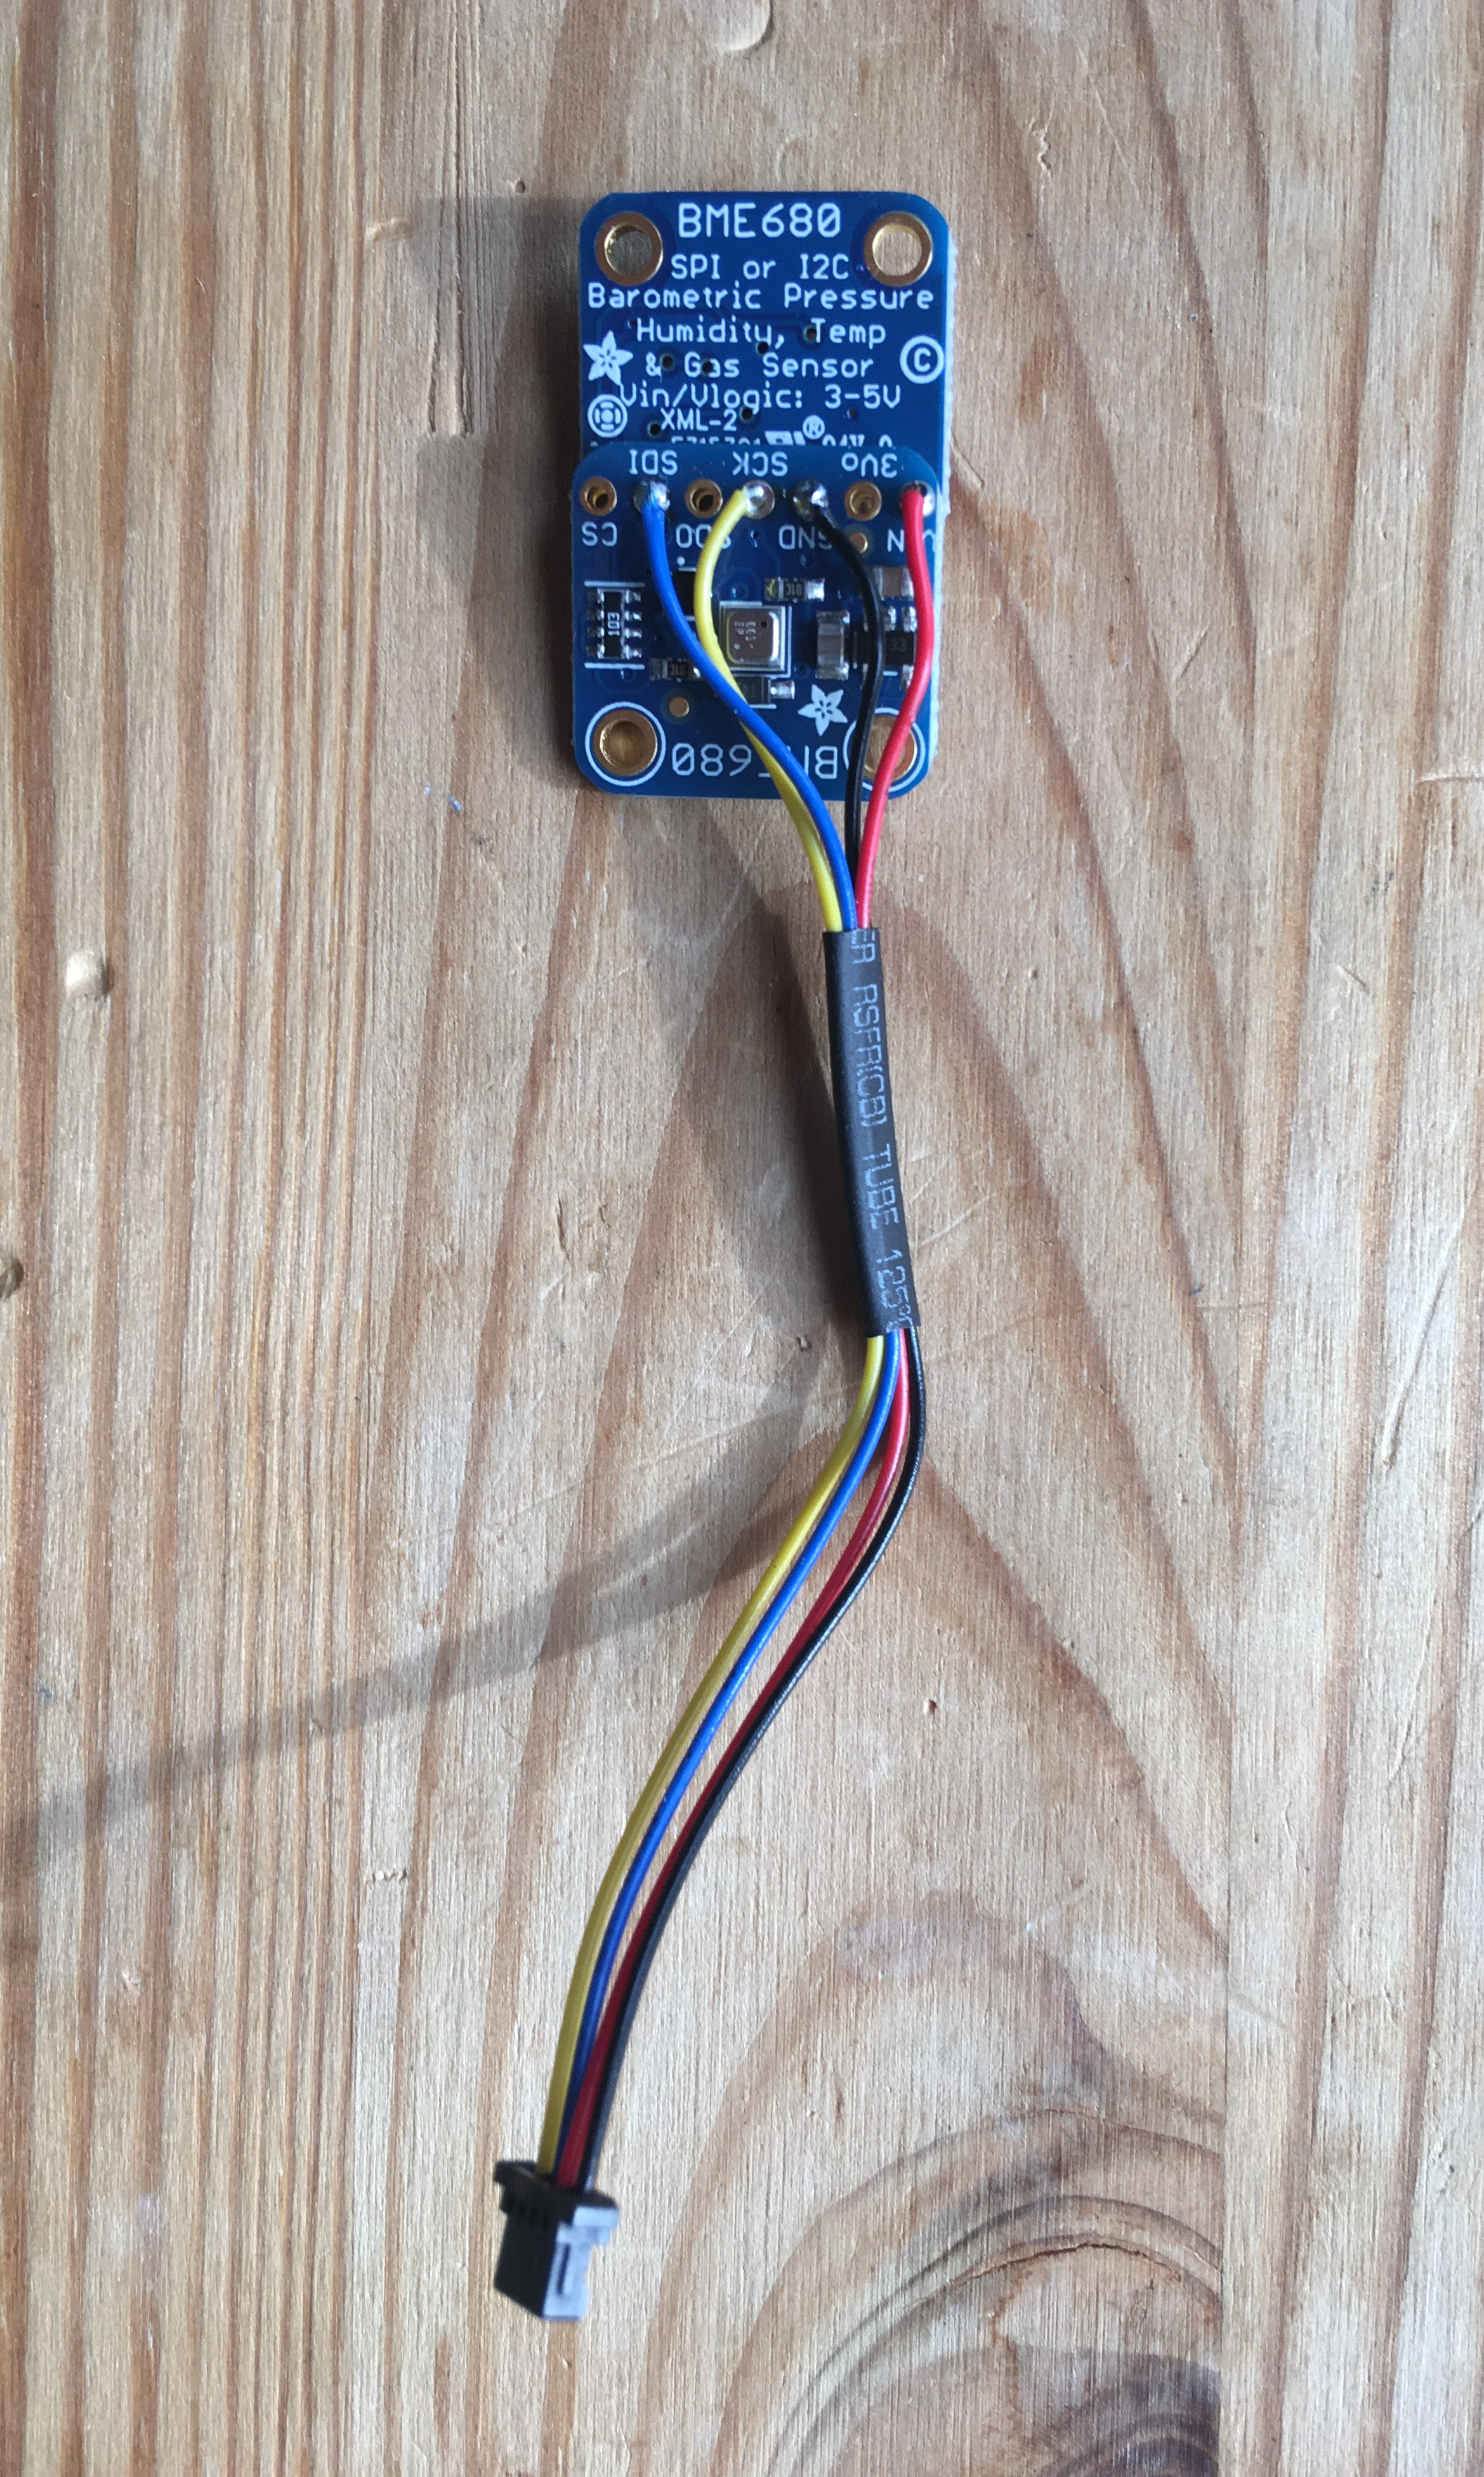
\includegraphics[width=0.65\textwidth]{images/bme_and_qwiic_cable.JPG}
\caption{Qwiic cable soldered to BME sensor assembly}
\end{figure}

\item
Add address jumper to ambient pressure sensor. Refer to figure \ref{fig:bme_diagram} on page \pageref{fig:bme_diagram}
\begin{enumerate}[label=3.5.\arabic*]
\item
Take a $1/2$" piece of hookup wire and strip both ends
\item
Flow the solder in the GND through hole and poke one end of the hook up wire into the hole
\item
Put the other end of the wire into the SDO through hole and apply solder
\end{enumerate}

\begin{figure}[H]
\centering
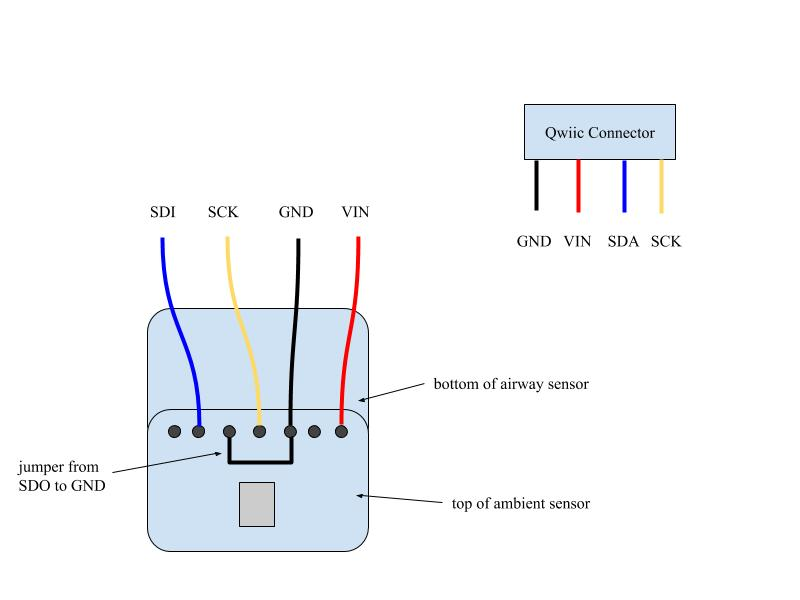
\includegraphics[width=0.75\textwidth]{images/bme_diagram.JPG}
\caption{Qwiic cable soldered to BME sensor assembly}
\label{fig:bme_diagram}
\end{figure}

\end{enumerate}

%-----------------------------------------------------------
% FLOW SENSOR
\item \label{itm:flow}
Flow Sensor Assembly

\begin{enumerate}[label=4.\arabic*]
\item
Assemble Cable. Refer to figure \ref{fig:flow_cable} on page \pageref{fig:flow_cable}

The flow sensor requires a 5 V input, however we will run the I$^2$C bus at 3.3 V necessitating this cable.
\\
\begin{enumerate}[label=4.1.\arabic*]
\item
Cut the Qwiic cable in half
\item
Cut off the red conductor near the base of the connector
\item
Cut a 30 cm length from the USB cable
\item
Strip the jacket back 1 $1/2$'' from one end
\item
Strip the first $1/4$'' of each conductor on one end and tin
\item
Twist a small portion of the shield into the black GND conductor
\item
Place a small piece of heat shrink on each conductor of the Qwicc cable and push them toward the connector end
\item
Solder the ends of the Qwiic cable to the ends of the USB cable following Table \ref{tab:flow}.
\begin{table}[H]
\centering
\begin{tabular}{| c | c | c |}
\hline
USB & Qwiic & Signal \\  \hline
black & black & GND \\  \hline
green & blue & SDA \\  \hline
white & yellow & SCK \\  \hline
red & single 6'' wire & 5V \\
\hline
\end{tabular}
\caption{flow sensor wiring}
\label{tab:flow}
\end{table}
\item
Connect the red wire to the red conductor in the USB cable and solder the extra long male header pin to the end
\item
Cover the finished joints with a short $1/4$'' piece of heat shrink
\end{enumerate}

\begin{figure}[H]
\centering
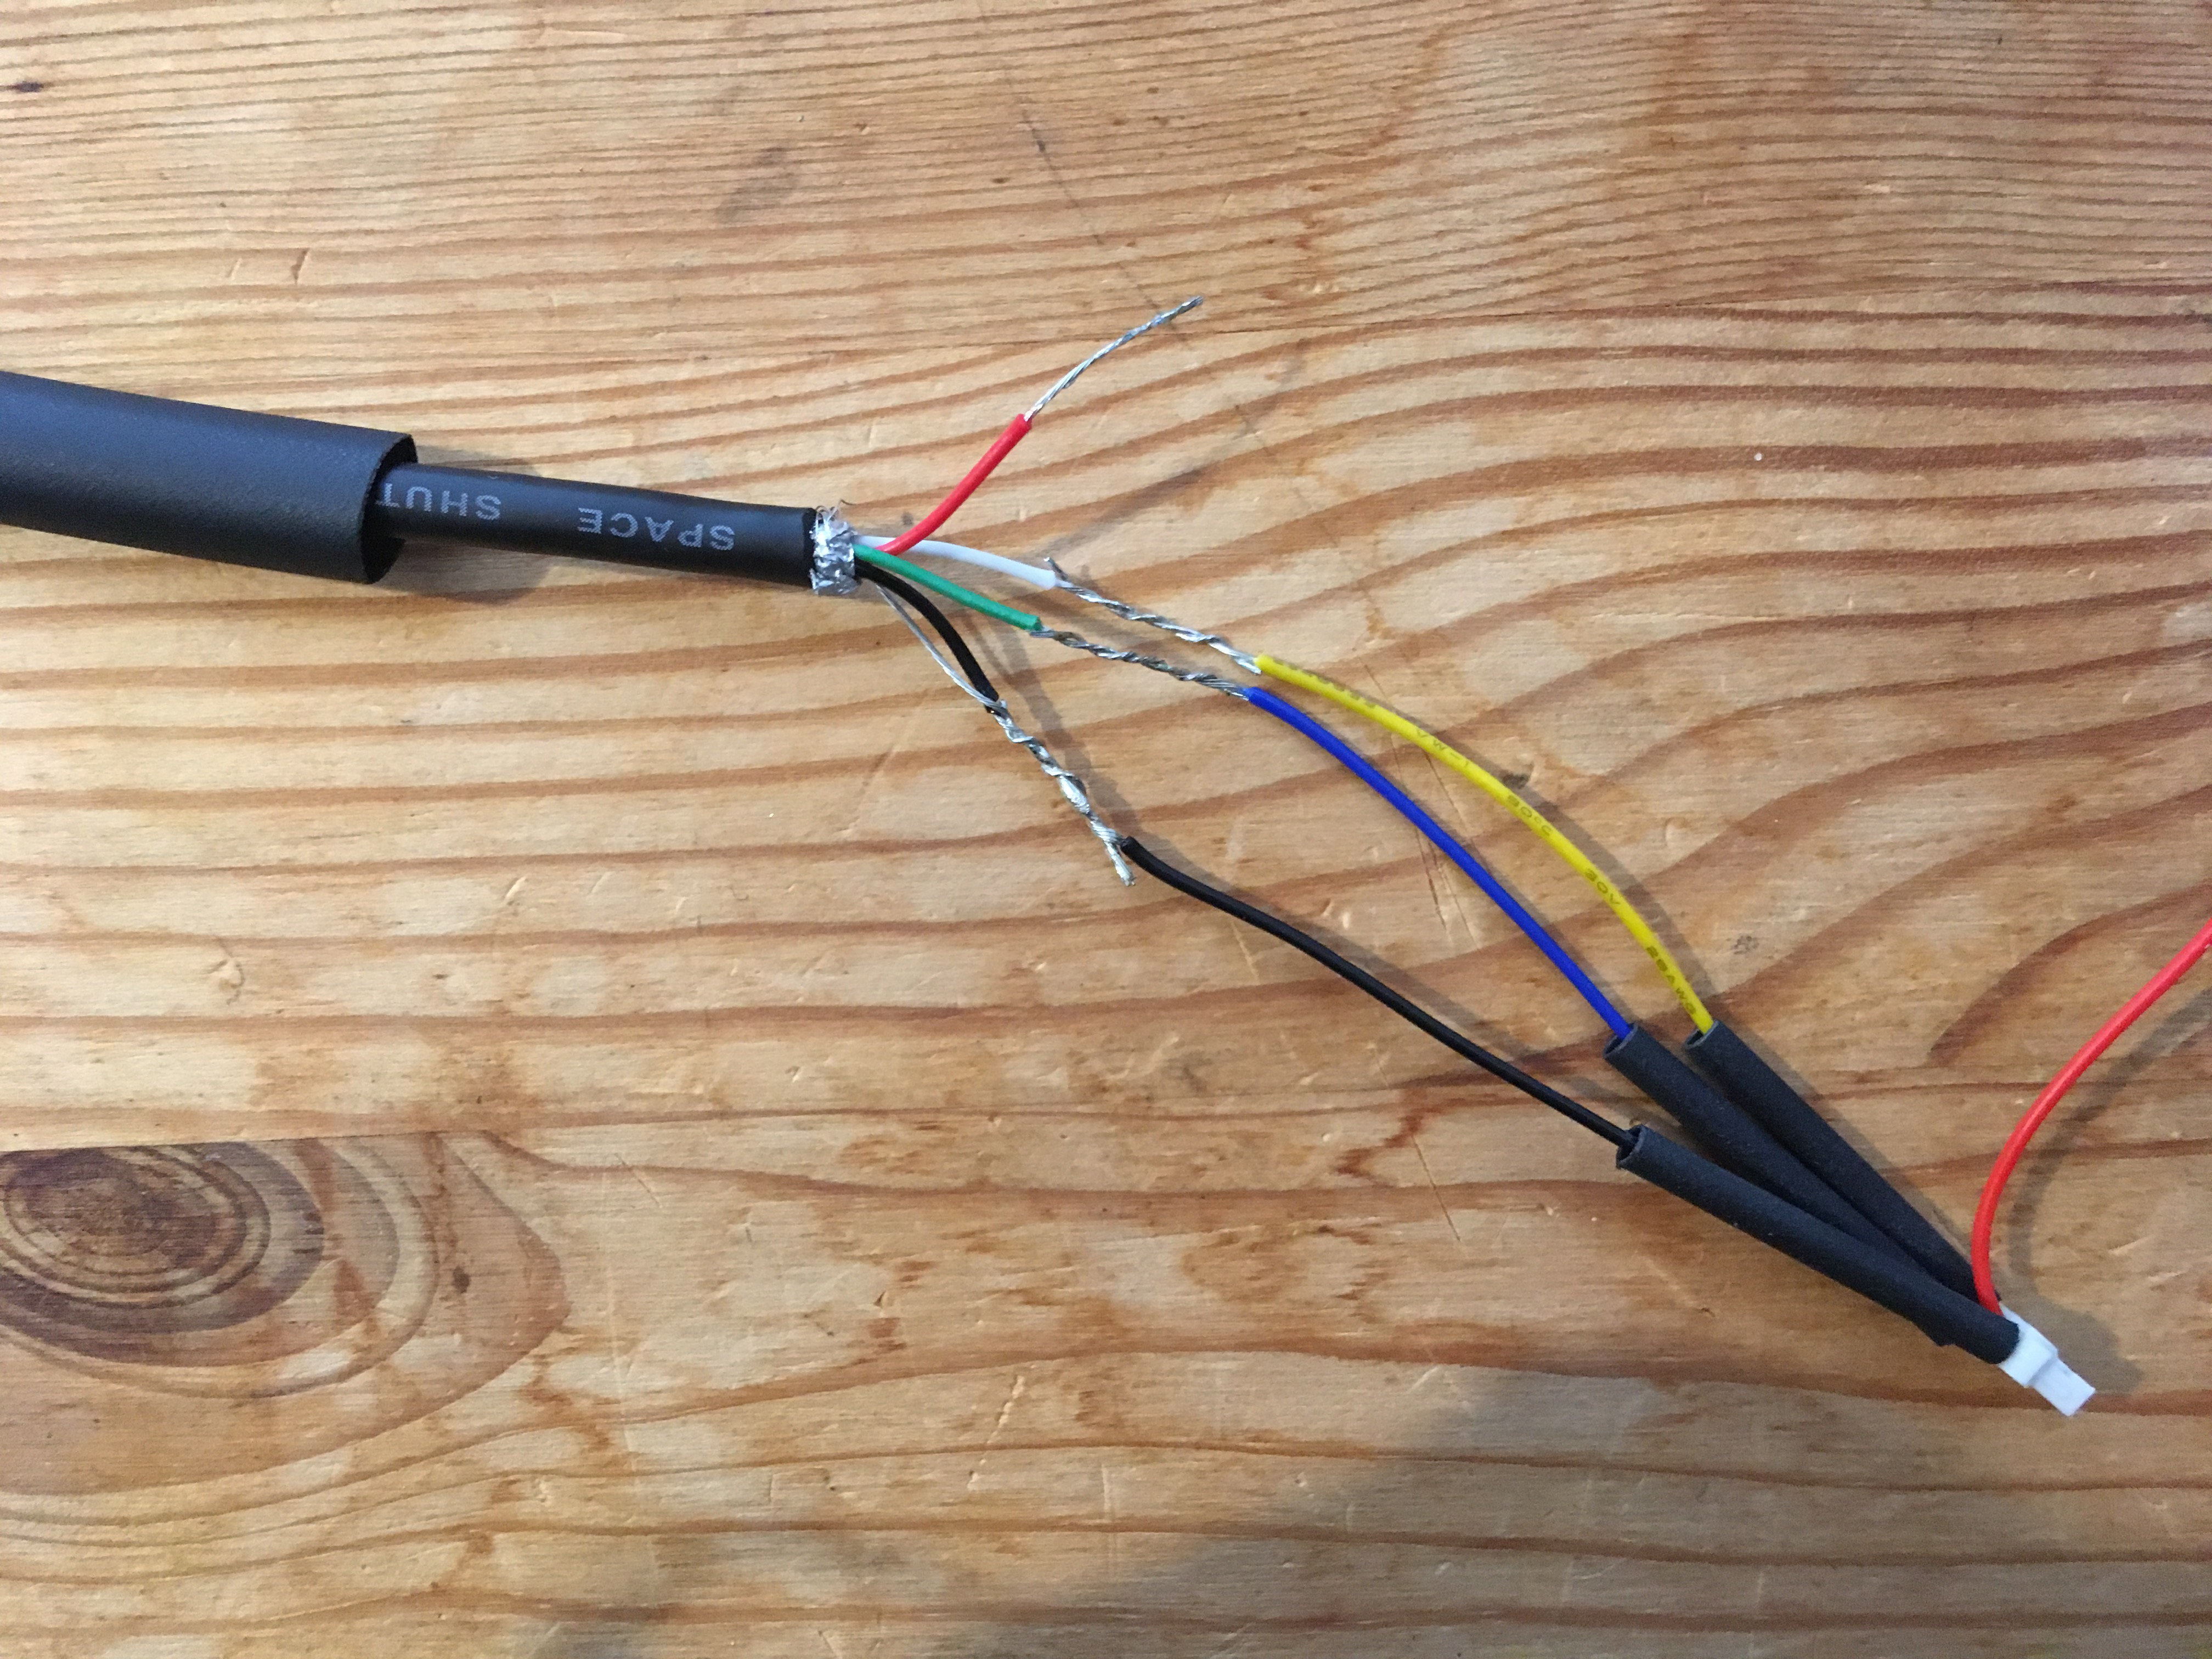
\includegraphics[width=0.45\textwidth]{images/flow_1.JPG}
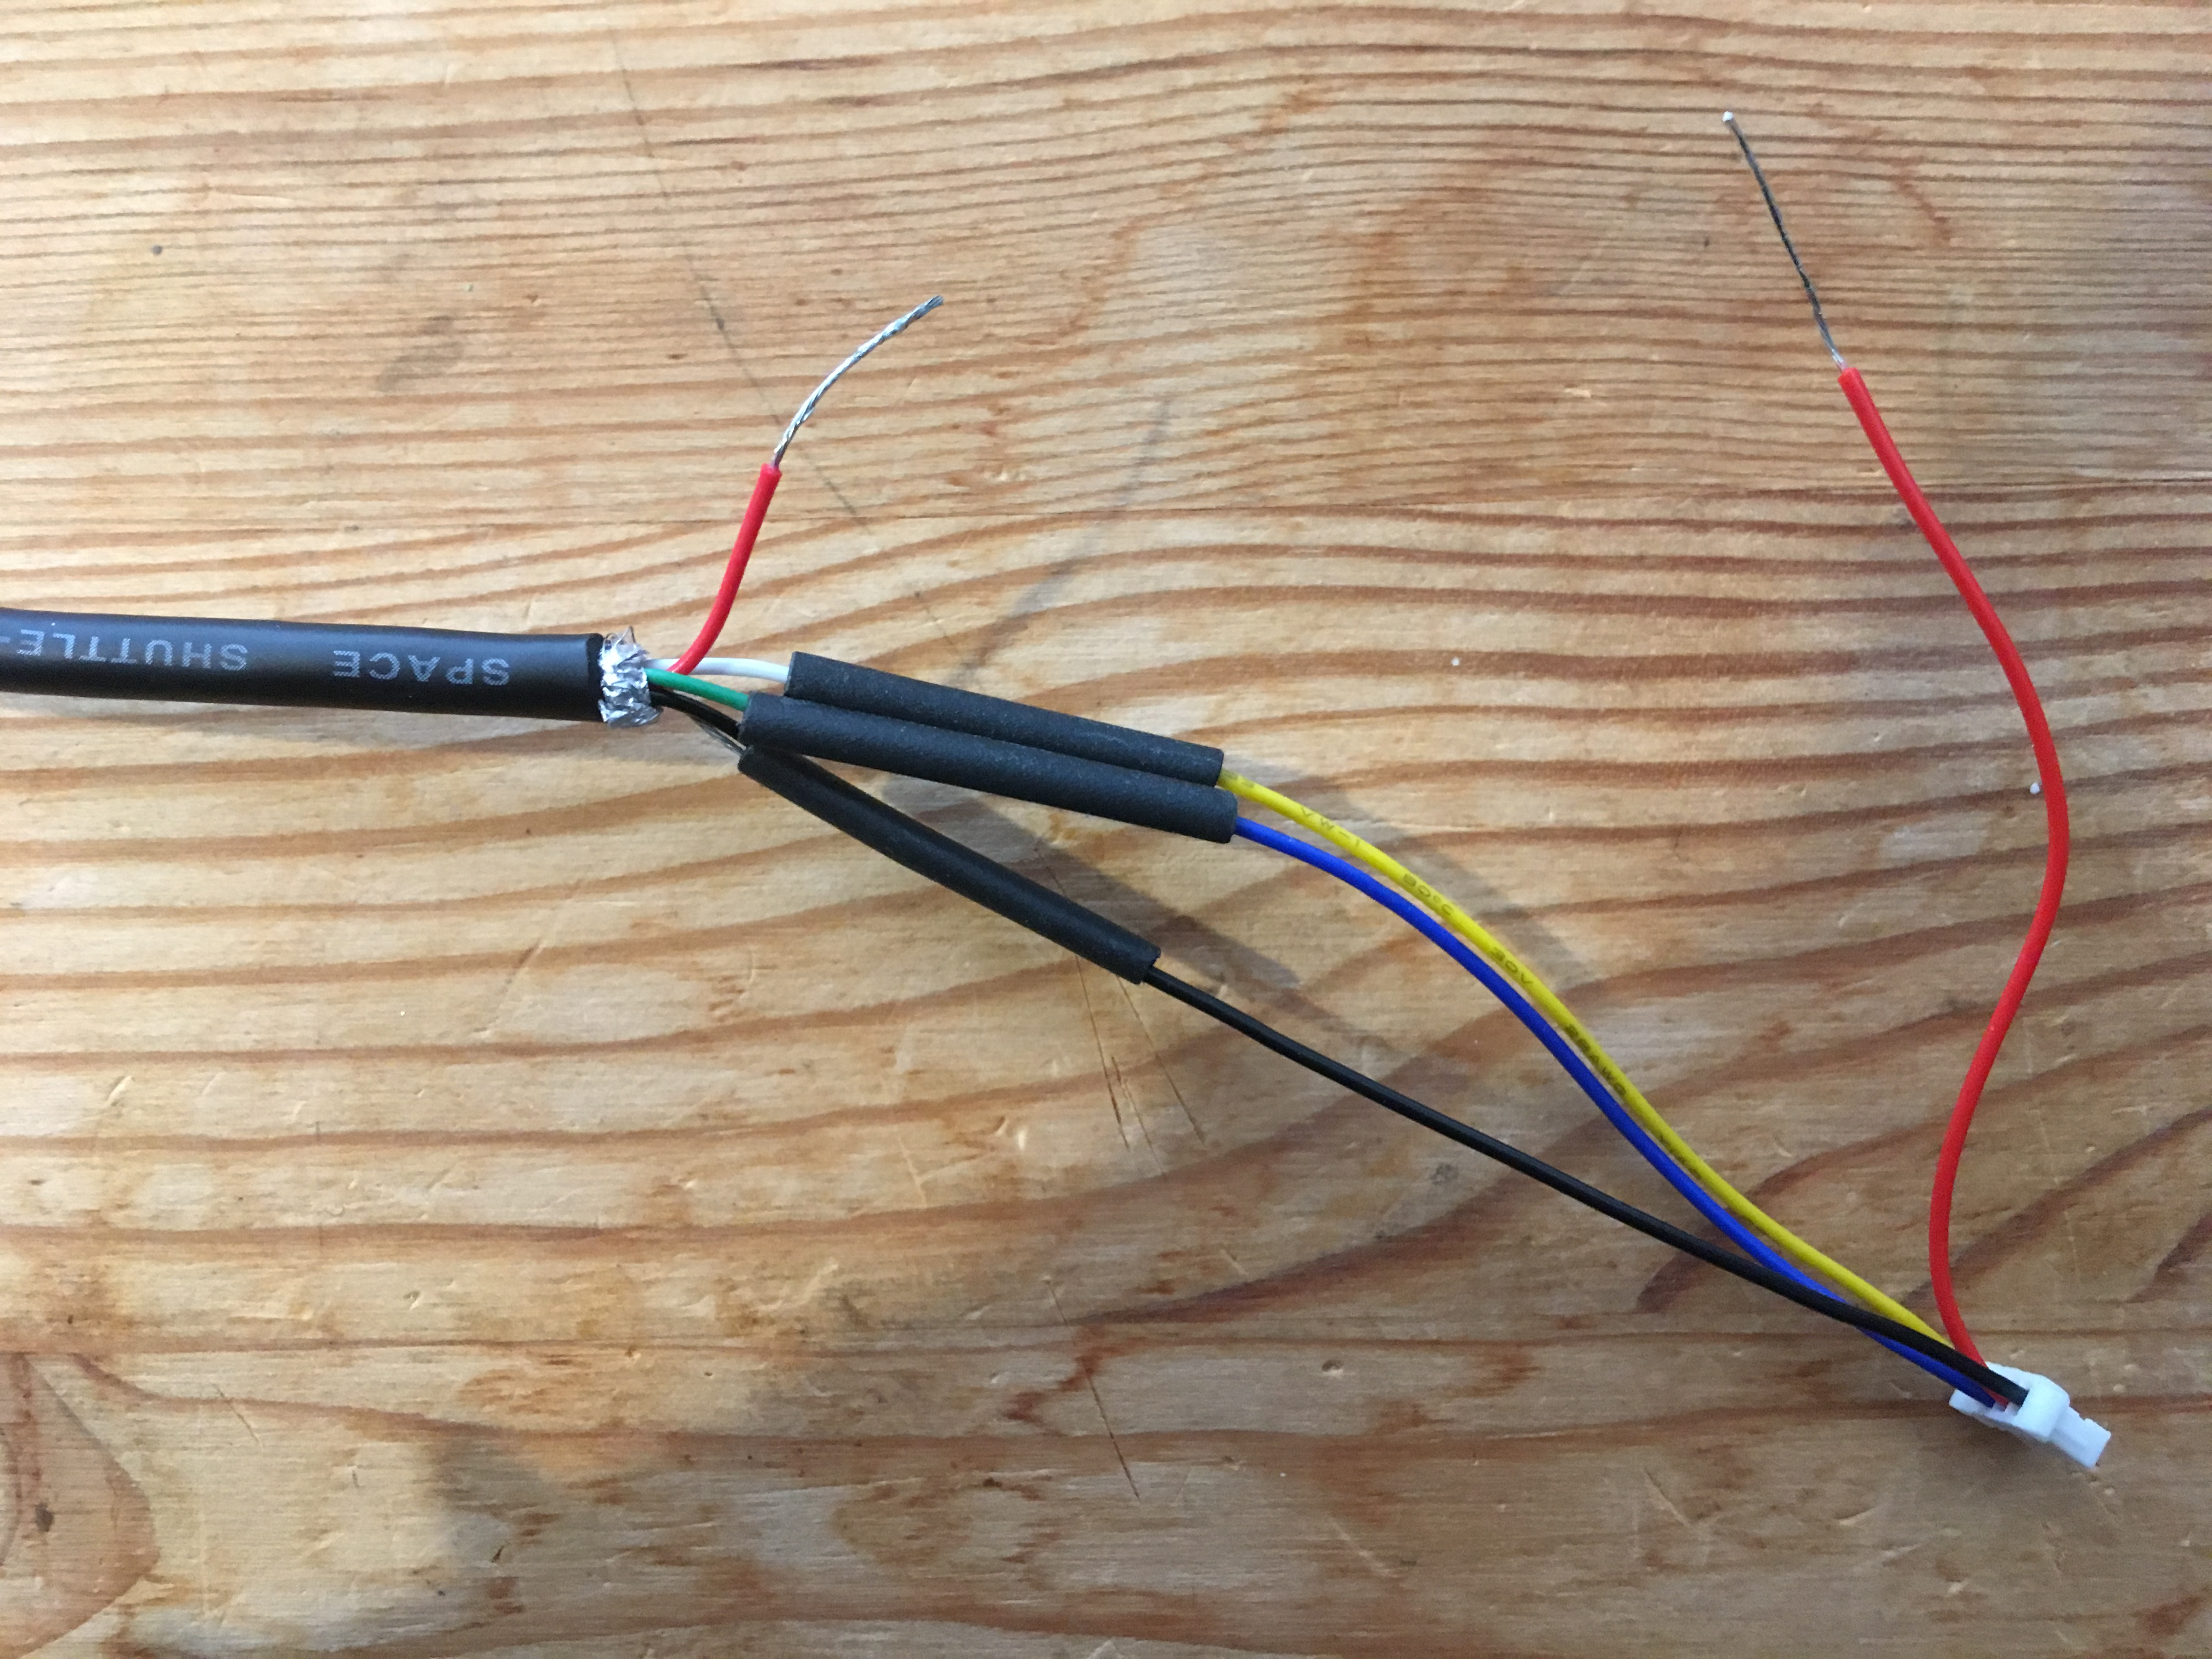
\includegraphics[width=0.45\textwidth]{images/flow_2.JPG} \\
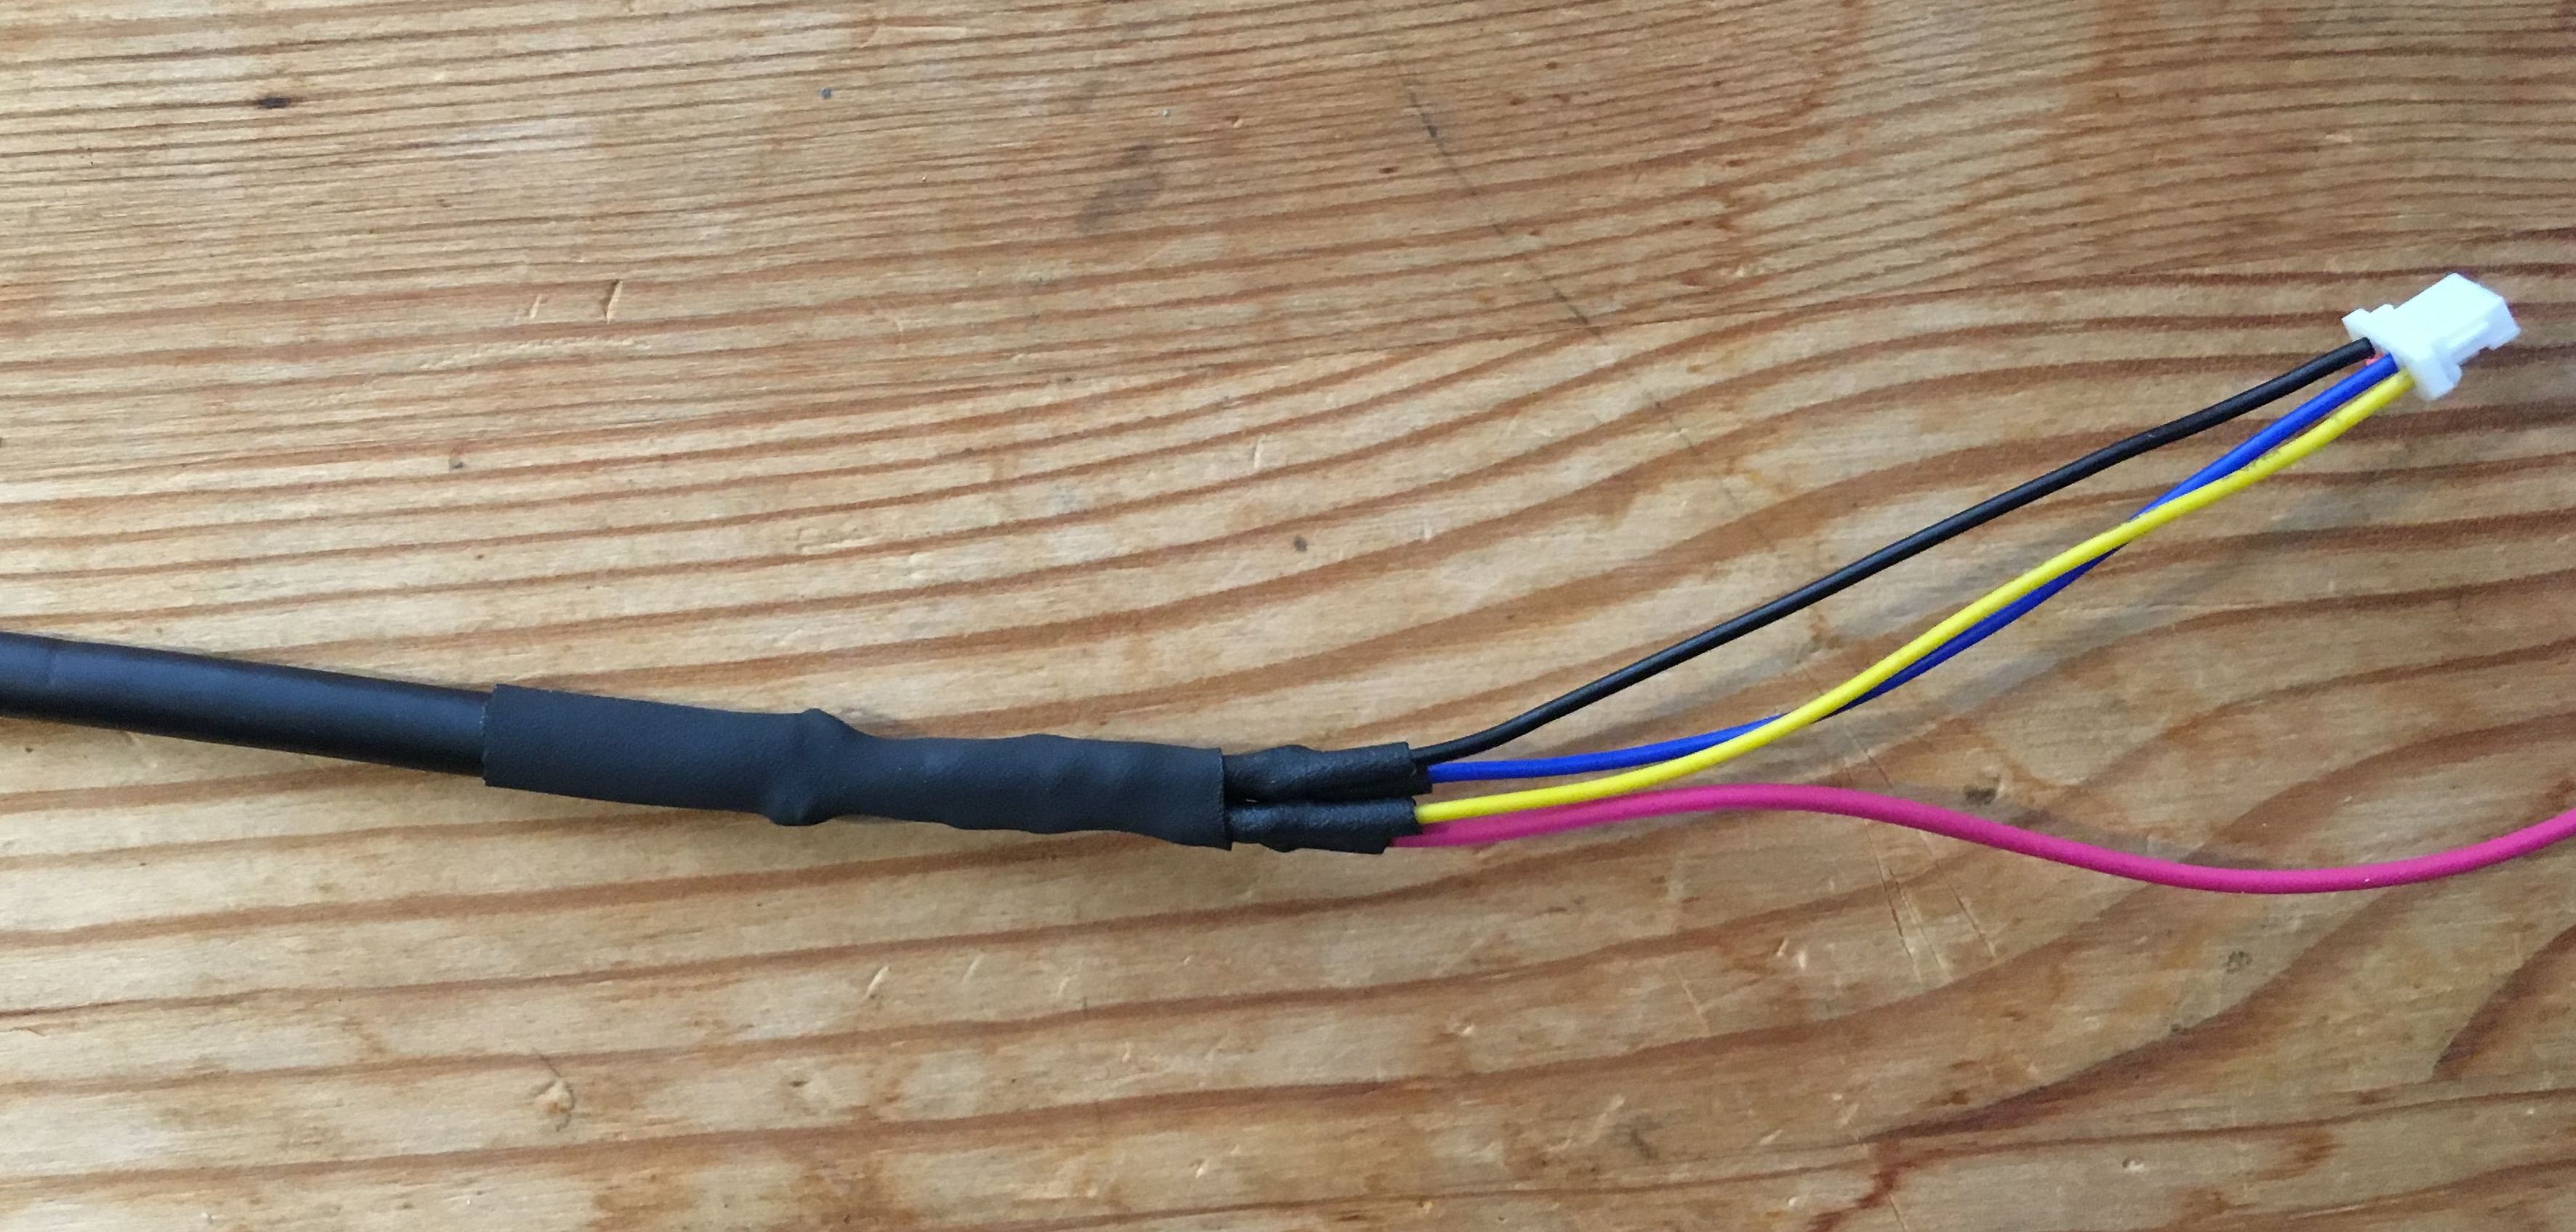
\includegraphics[width=0.45\textwidth]{images/flow_4.JPG}
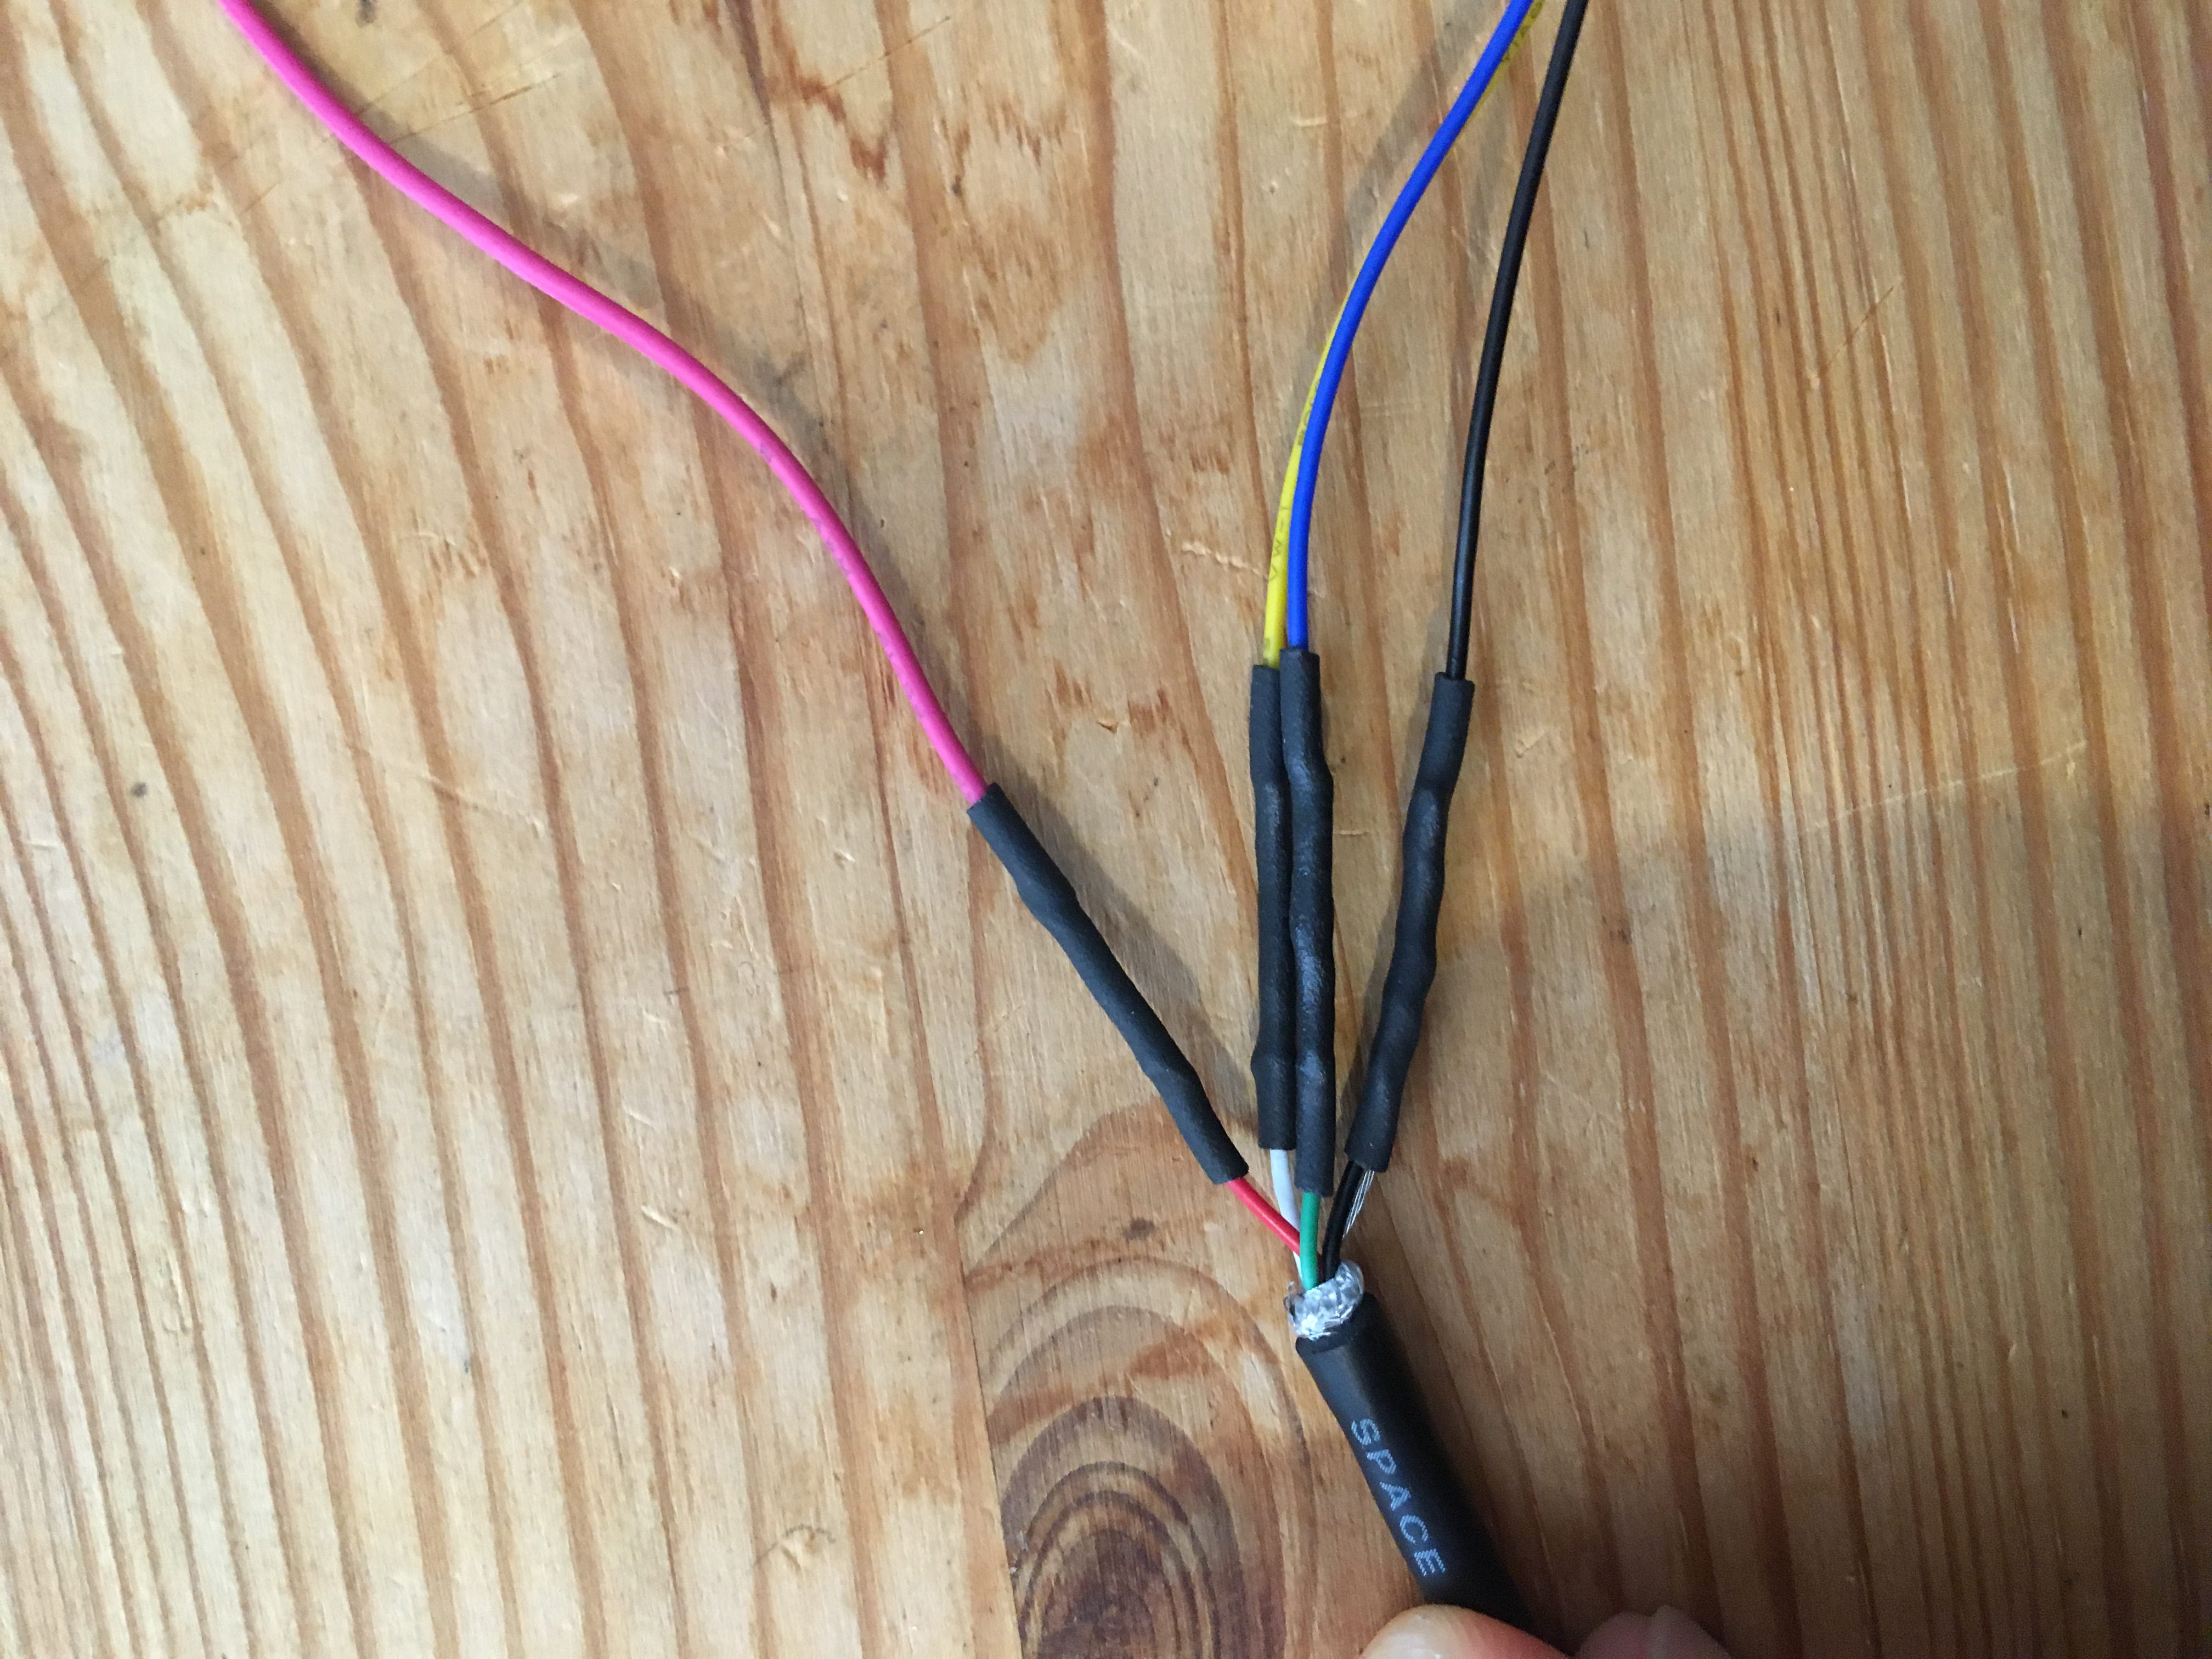
\includegraphics[width=0.45\textwidth]{images/flow_3.JPG}
\caption{Clockwise progression of sensor cable assembly.}
\label{fig:flow_cable}
\end{figure}

\item
Connect cable to sensor.  Refer to figure \ref{fig:flow_sensor} on page \pageref{fig:flow_sensor}.

\begin{enumerate}[label=4.2.\arabic*]
\item
Apply a small quantity of solder to the four center pads on the SFM3400 flow sensor
\item
Remove $5/8$'' of the jacket on the bare end of the USB cable
\item
Strip back $1/8$'' from each conductor and tin the ends
\item
Thread the cable through the hole in the sensor as shown in the photo and make sure the tinned leads can reach the sensor pads
\item
Connect the end of each lead to the pads you have prepared by touching the tip of the soldering iron to the pad and then placing the tinned lead onto it.
\item
Refer to the SFM3400 datasheet to be sure you are connecting them in the proper position.
\end{enumerate}
\begin{figure}[H]
\label{fig:flow_sensor}
\centering
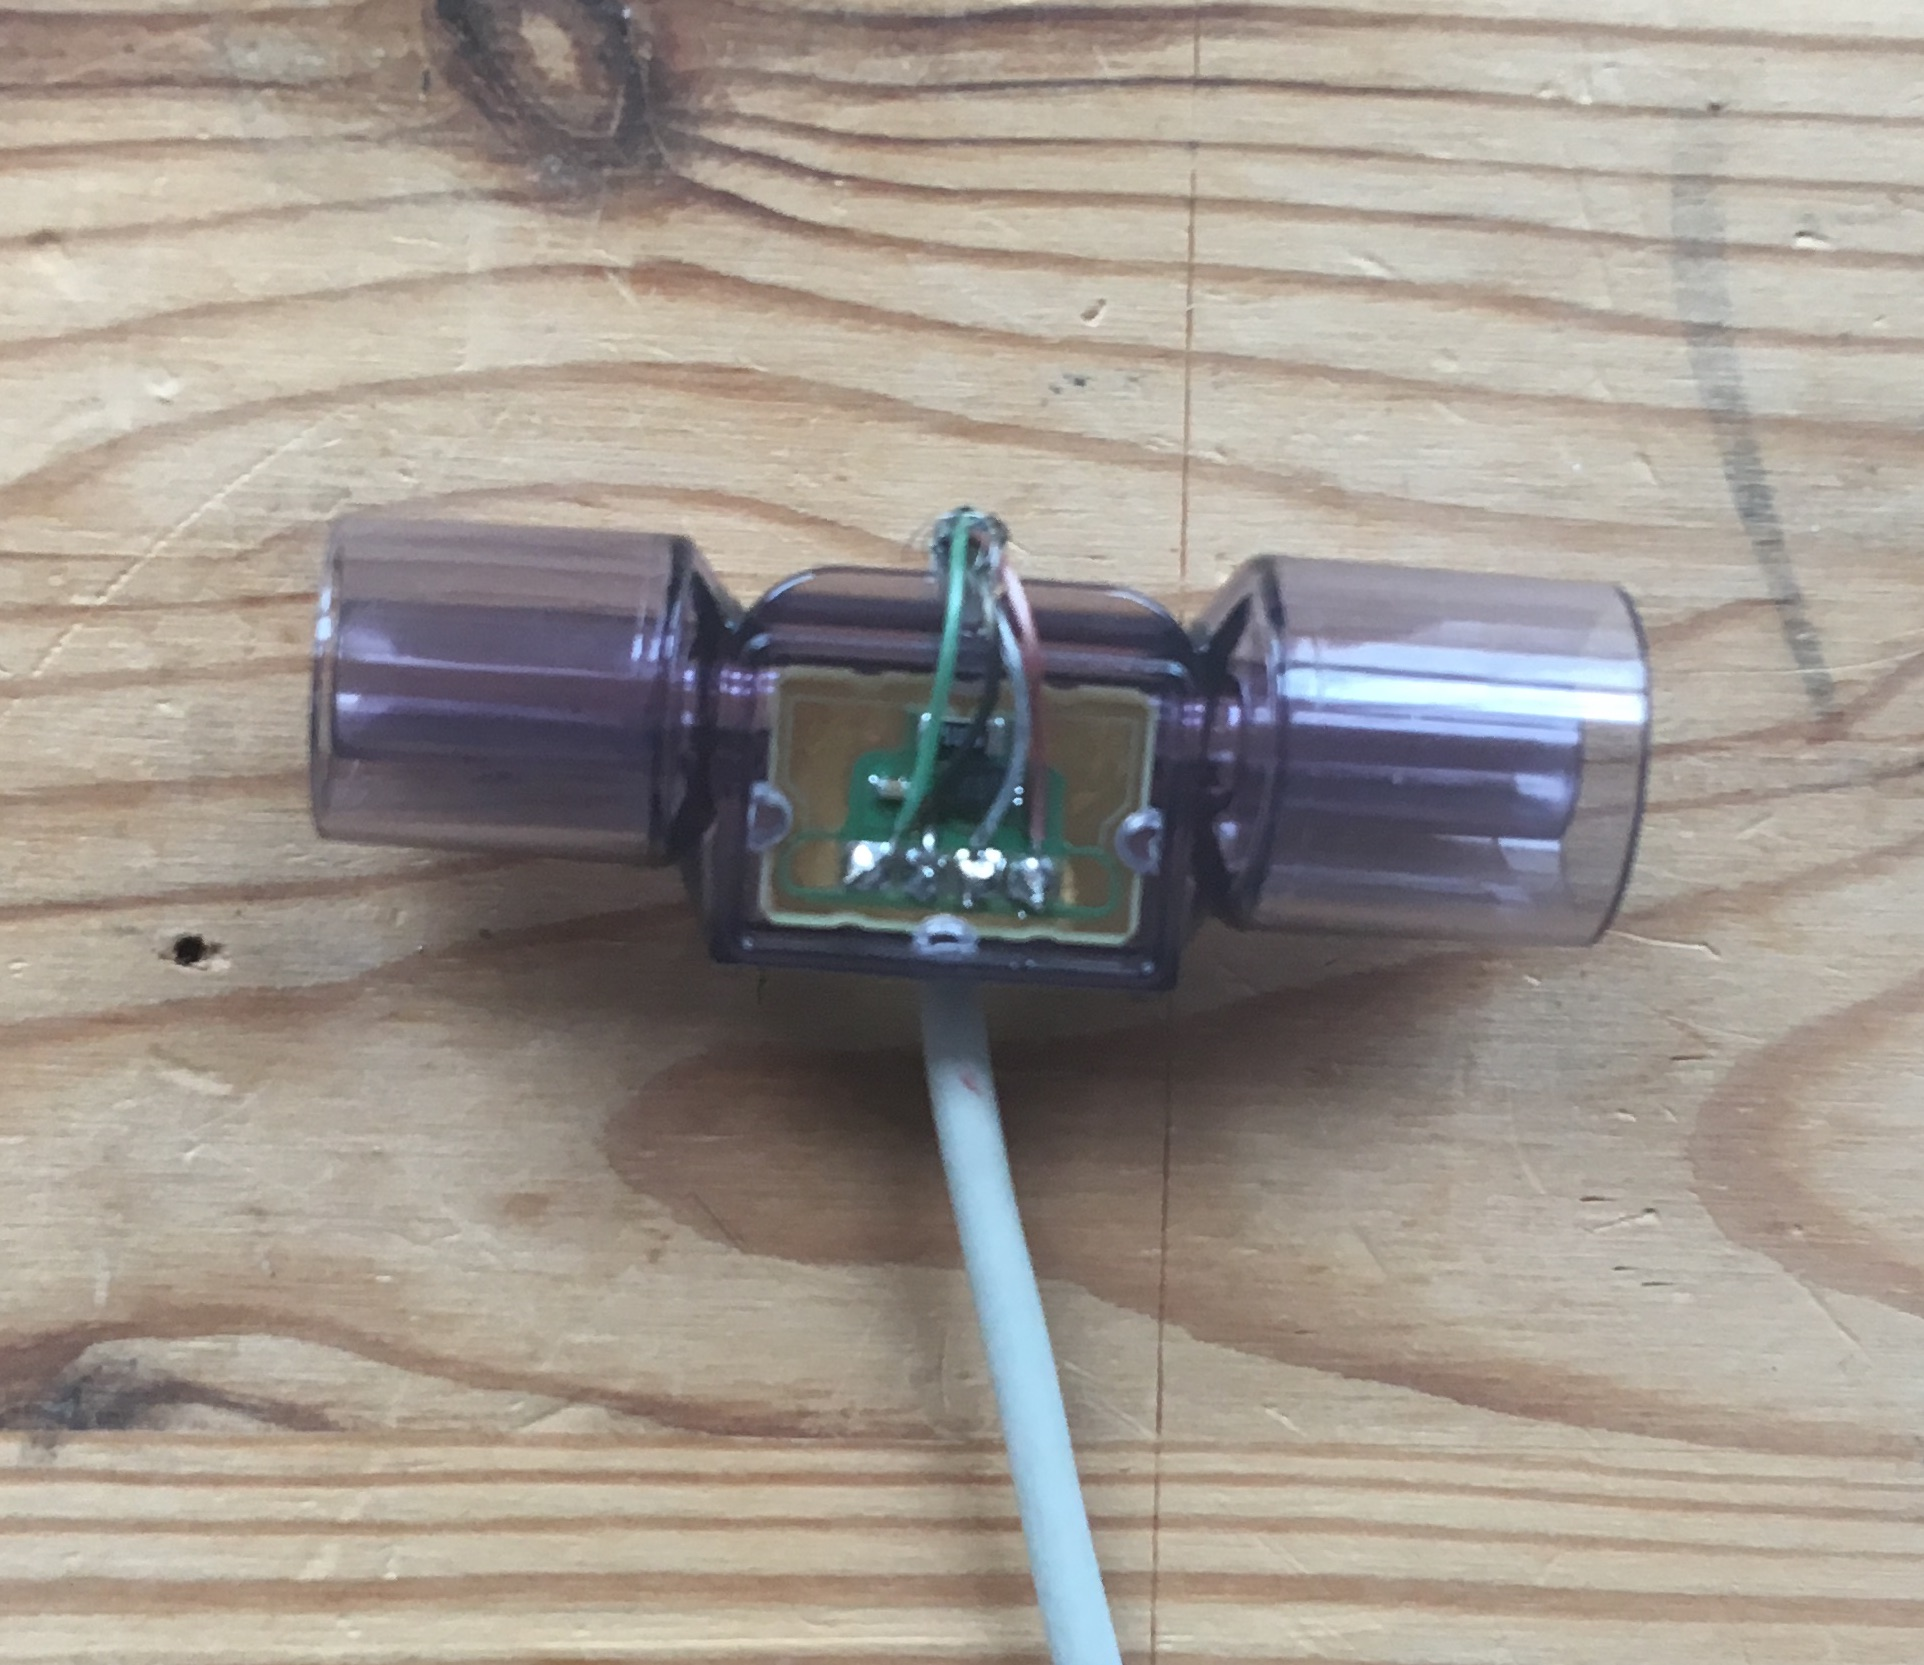
\includegraphics[width=0.6\textwidth]{images/flow_cable.JPG}
\caption{Sensor connected to cable assembly.}
\end{figure}

\item
  Assemble sensor adaptors. Refer to figure \ref{fig:adaptors} on page \pageref{fig:adaptors}.
  {\em NOTE: These photos and the 15mm adaptor show and refer to the neonatal version of the Sensirion flow sensor (SFM3400),
    which we used only because the adult-sized versions were impossible to find (temporarily). However, they physical
    assembly is exactly the same for all versions. You will not need the 15mm to 22mm adaptor with an adult-sized flow sensor.}

\begin{enumerate}[label=4.3.\arabic*]
\item
Cut a 1 $1/2$'' section of petex tubing
\item
Insert the tubing into the wide end of the flow sensor
\item
Insert the frosted 15 mm to 22 mm adaptor over the petex
\item
Add the clear 15 mm to 22 mm adaptor over the small end of the flow sensor
\item
Place the bleed adaptor over the clear adaptor
\item
Use electrical tape to secure any loose connections
\end{enumerate}
\begin{figure}[H]
\centering
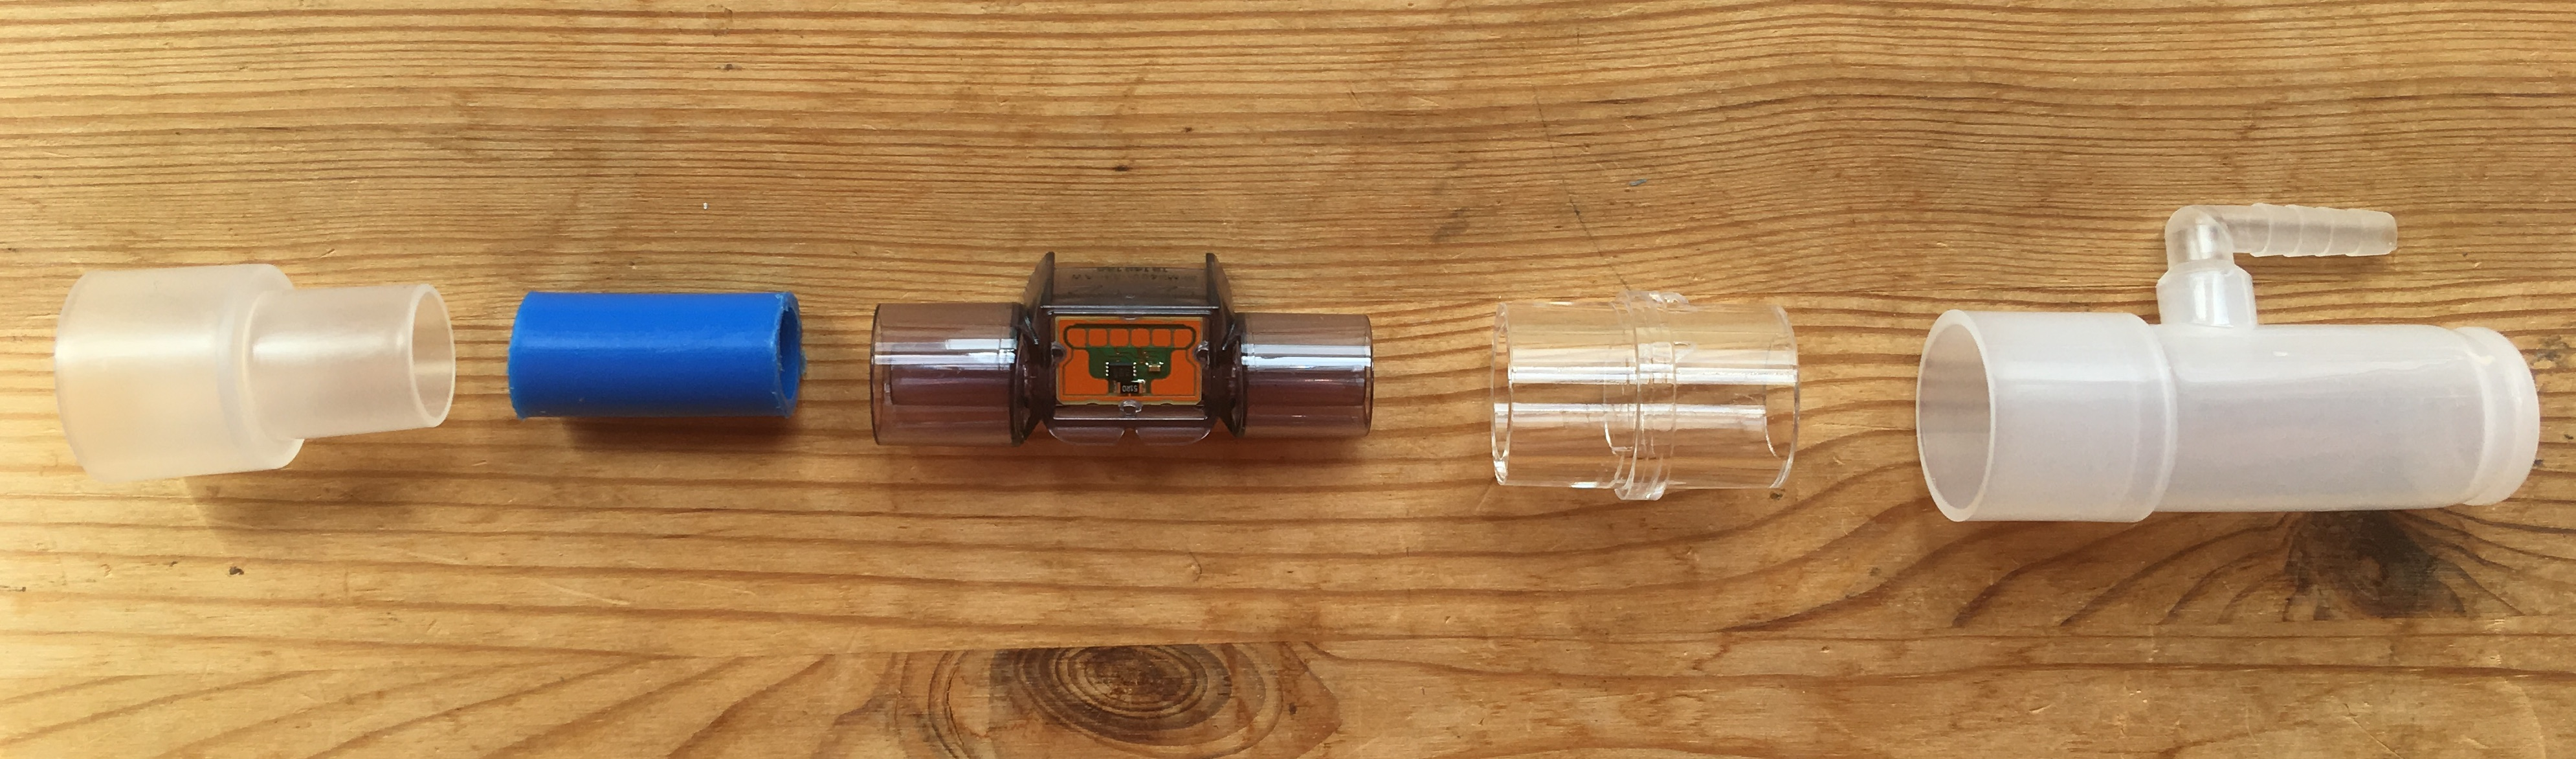
\includegraphics[width=0.8\textwidth]{images/adapters_1.JPG} \\
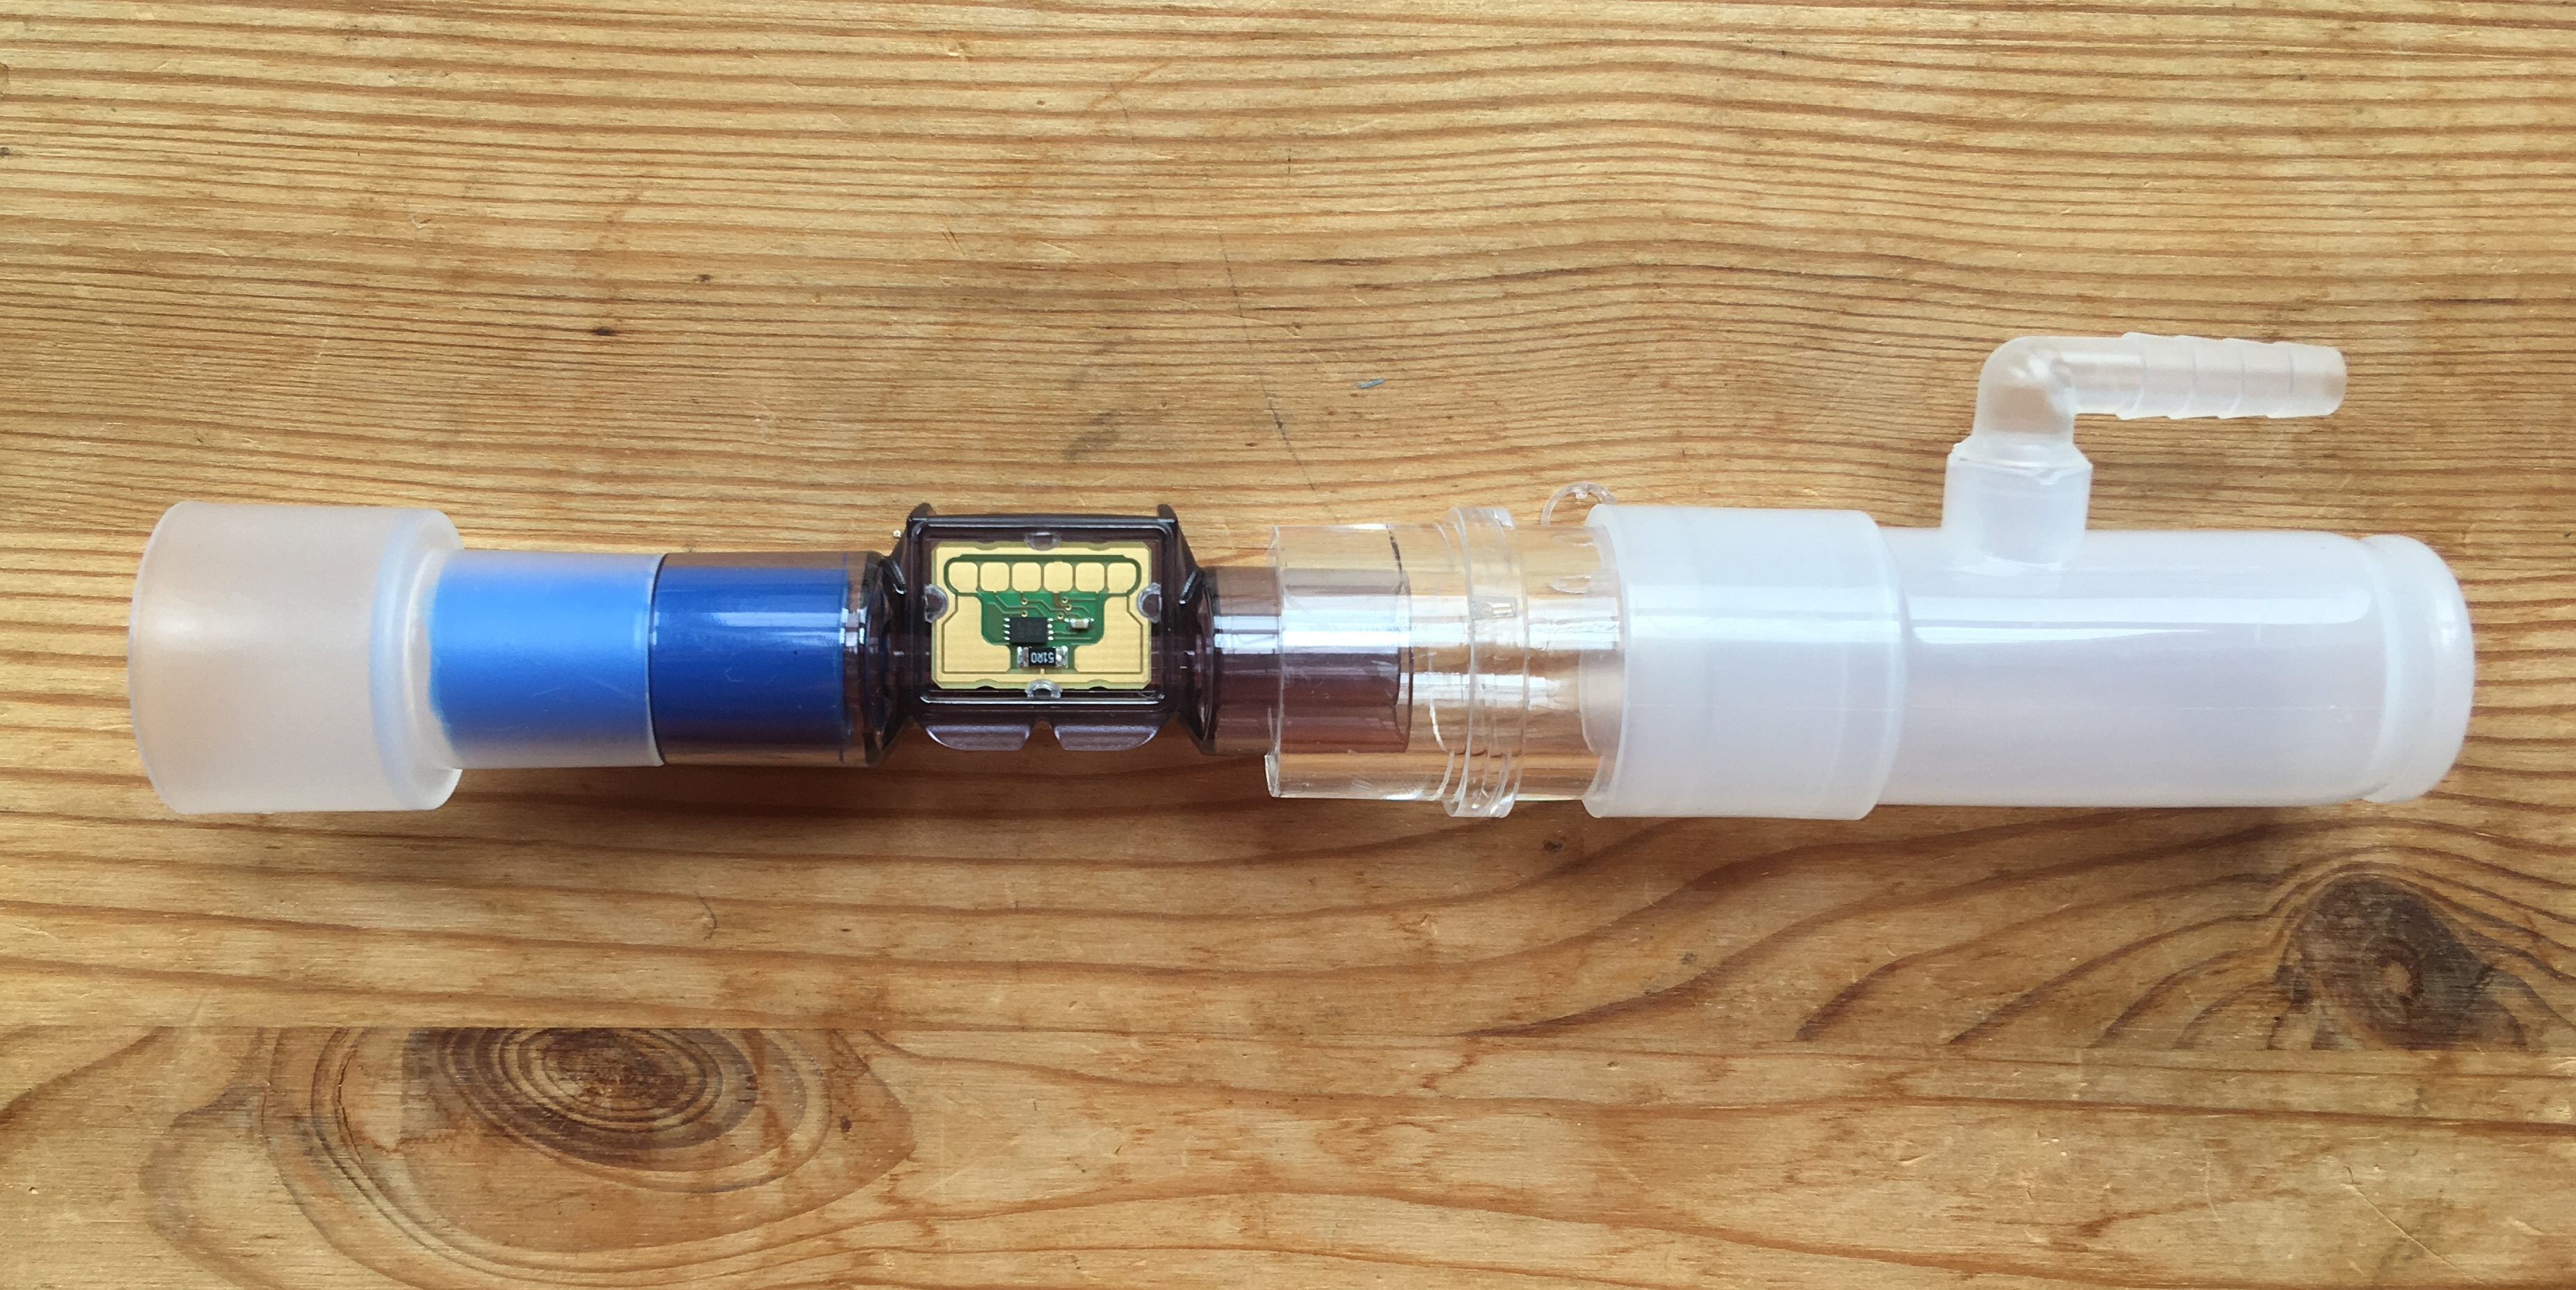
\includegraphics[width=0.6\textwidth]{images/adapters_2.JPG} \\
\caption{Adaptors assembled inline with sensor.}
\label{fig:adaptors}
\end{figure}

\end{enumerate}

%-----------------------------------------------------------
% FINAL ASSEMBLY
\item
Final Assembly

\begin{enumerate}[label=5.\arabic*]
\item
Glue oxygen hose to pressure sensor assembly. Refer to figure \ref{fig:bme_glue} on page \pageref{fig:bme_glue}.

\begin{enumerate}[label=5.1.\arabic*]
\item
Cut a section of oxygen hose approximately the same length as the flow sensor cable
\item
Make sure your cut is flat on the end
\item
Place one end of the hose over the internal, breathing circuit pressure sensor and apply glue around the edges
\item
Be very careful not to get glue on the sensor and make sure that the hose is securely attached to the pcb
\end{enumerate}
\begin{figure}[H]
\centering
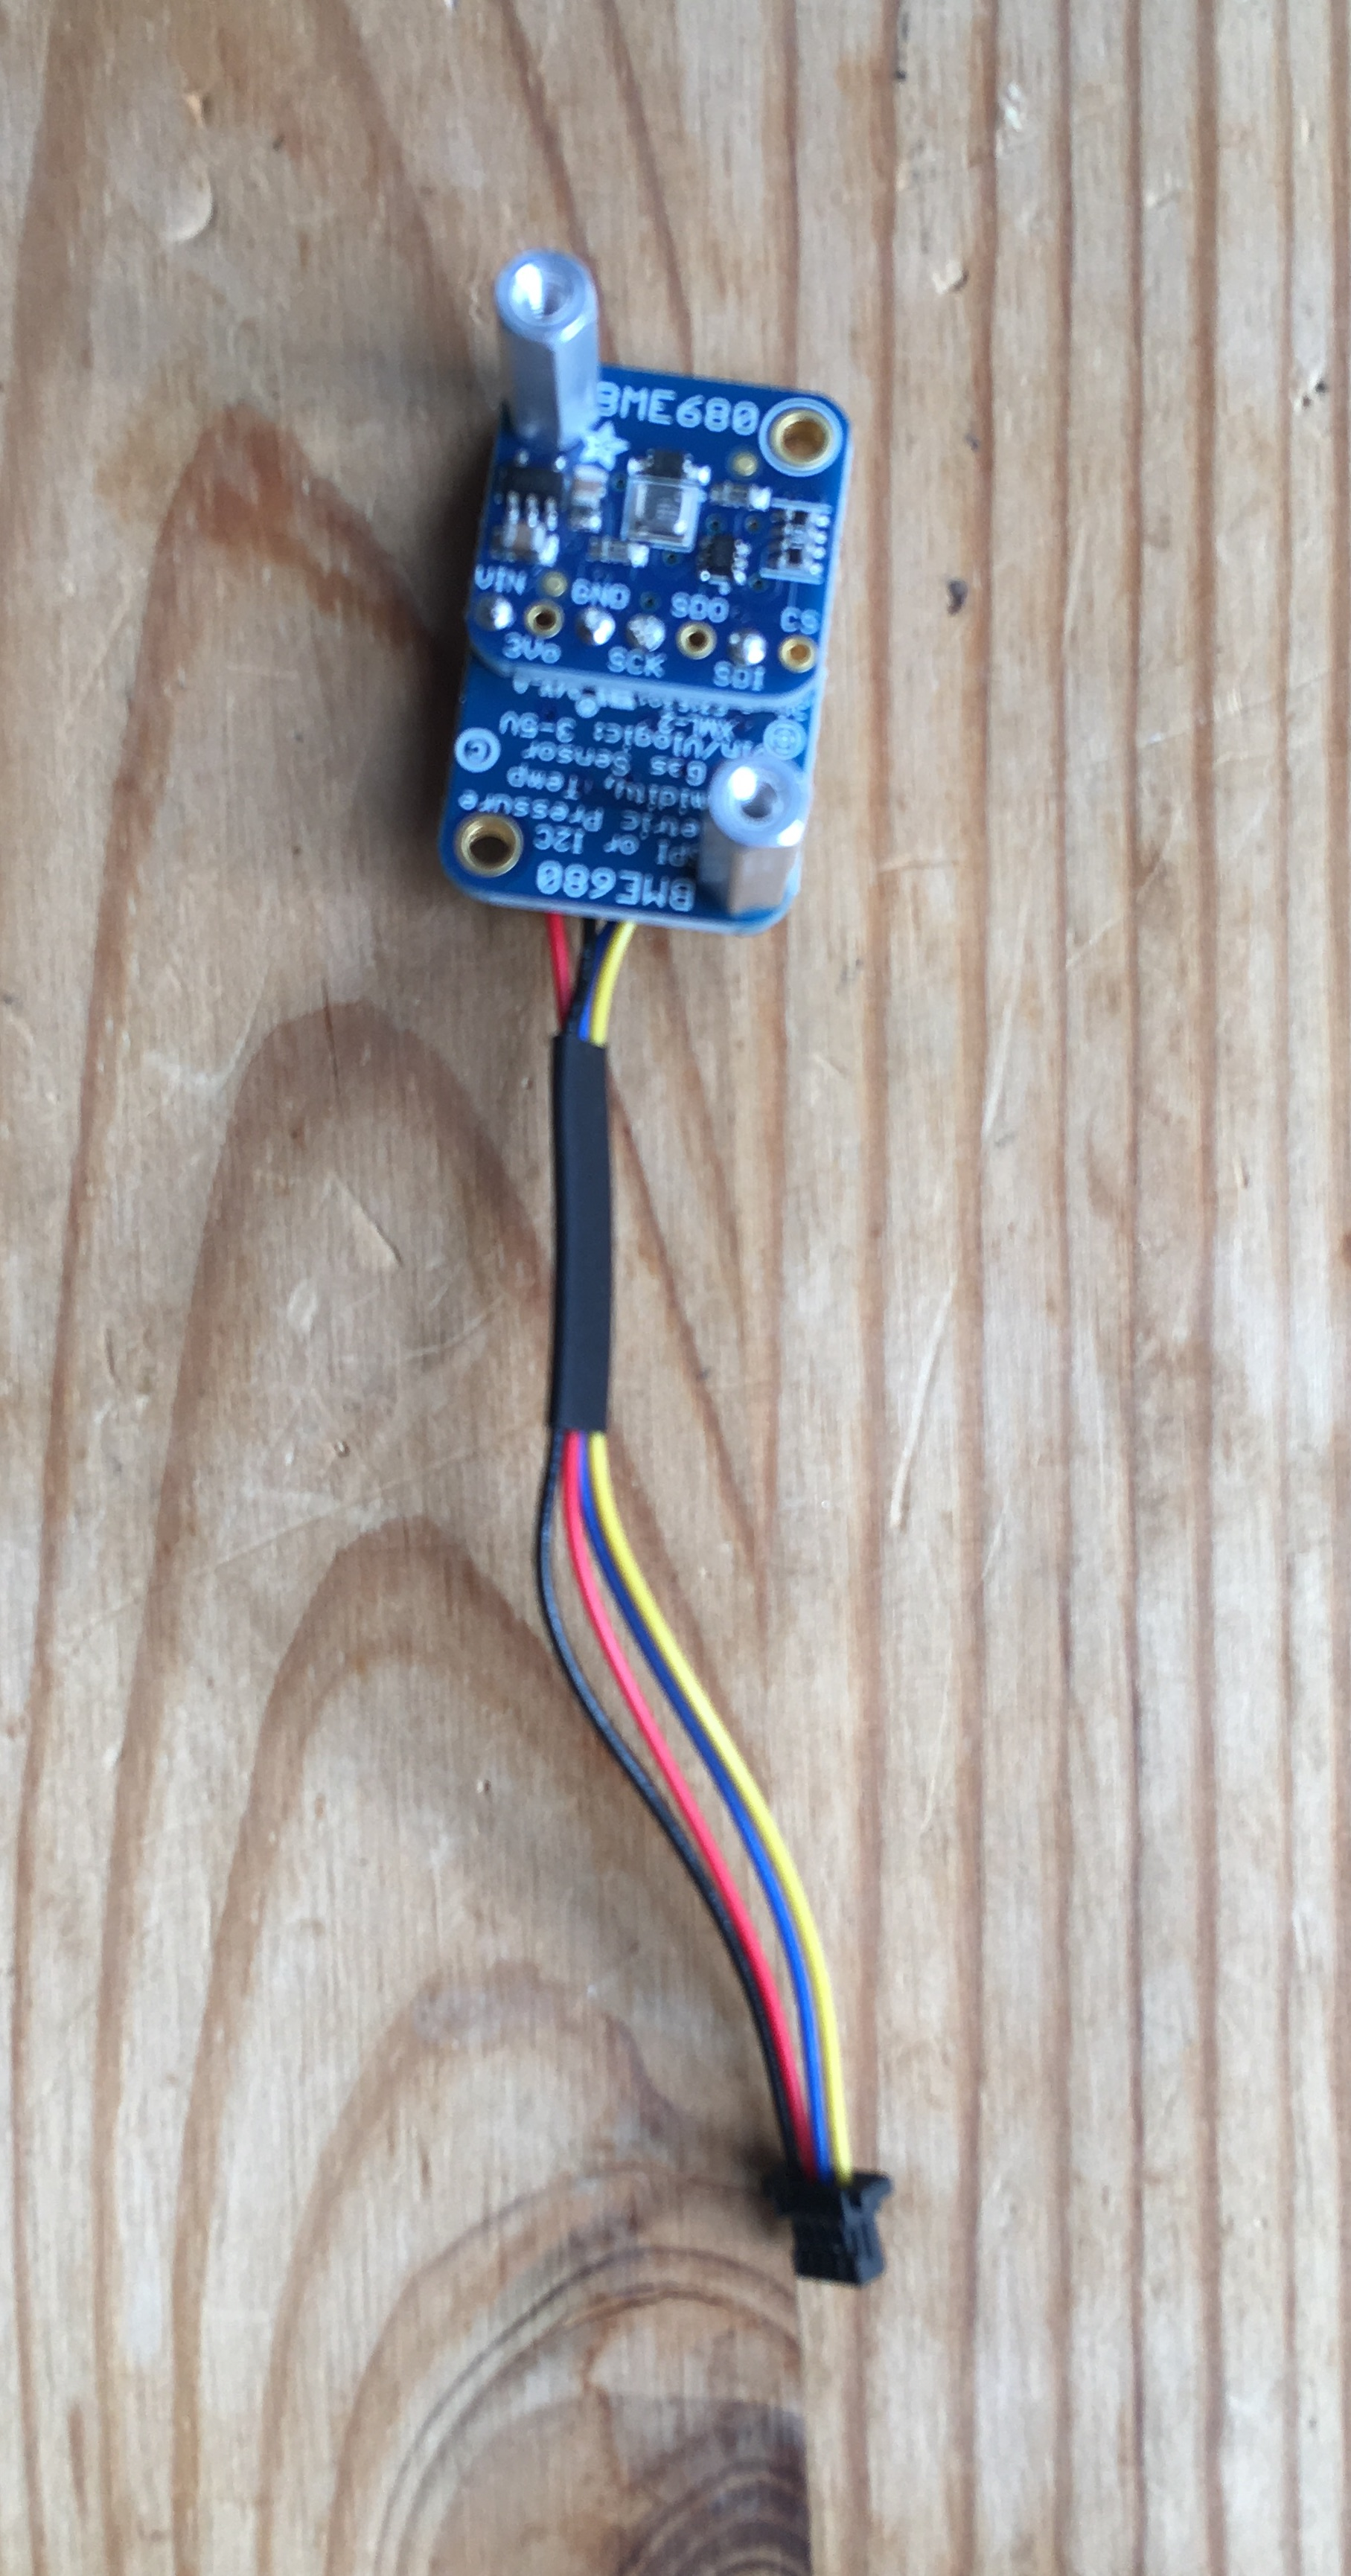
\includegraphics[width=0.4\textwidth]{images/bme_standoffs.JPG}
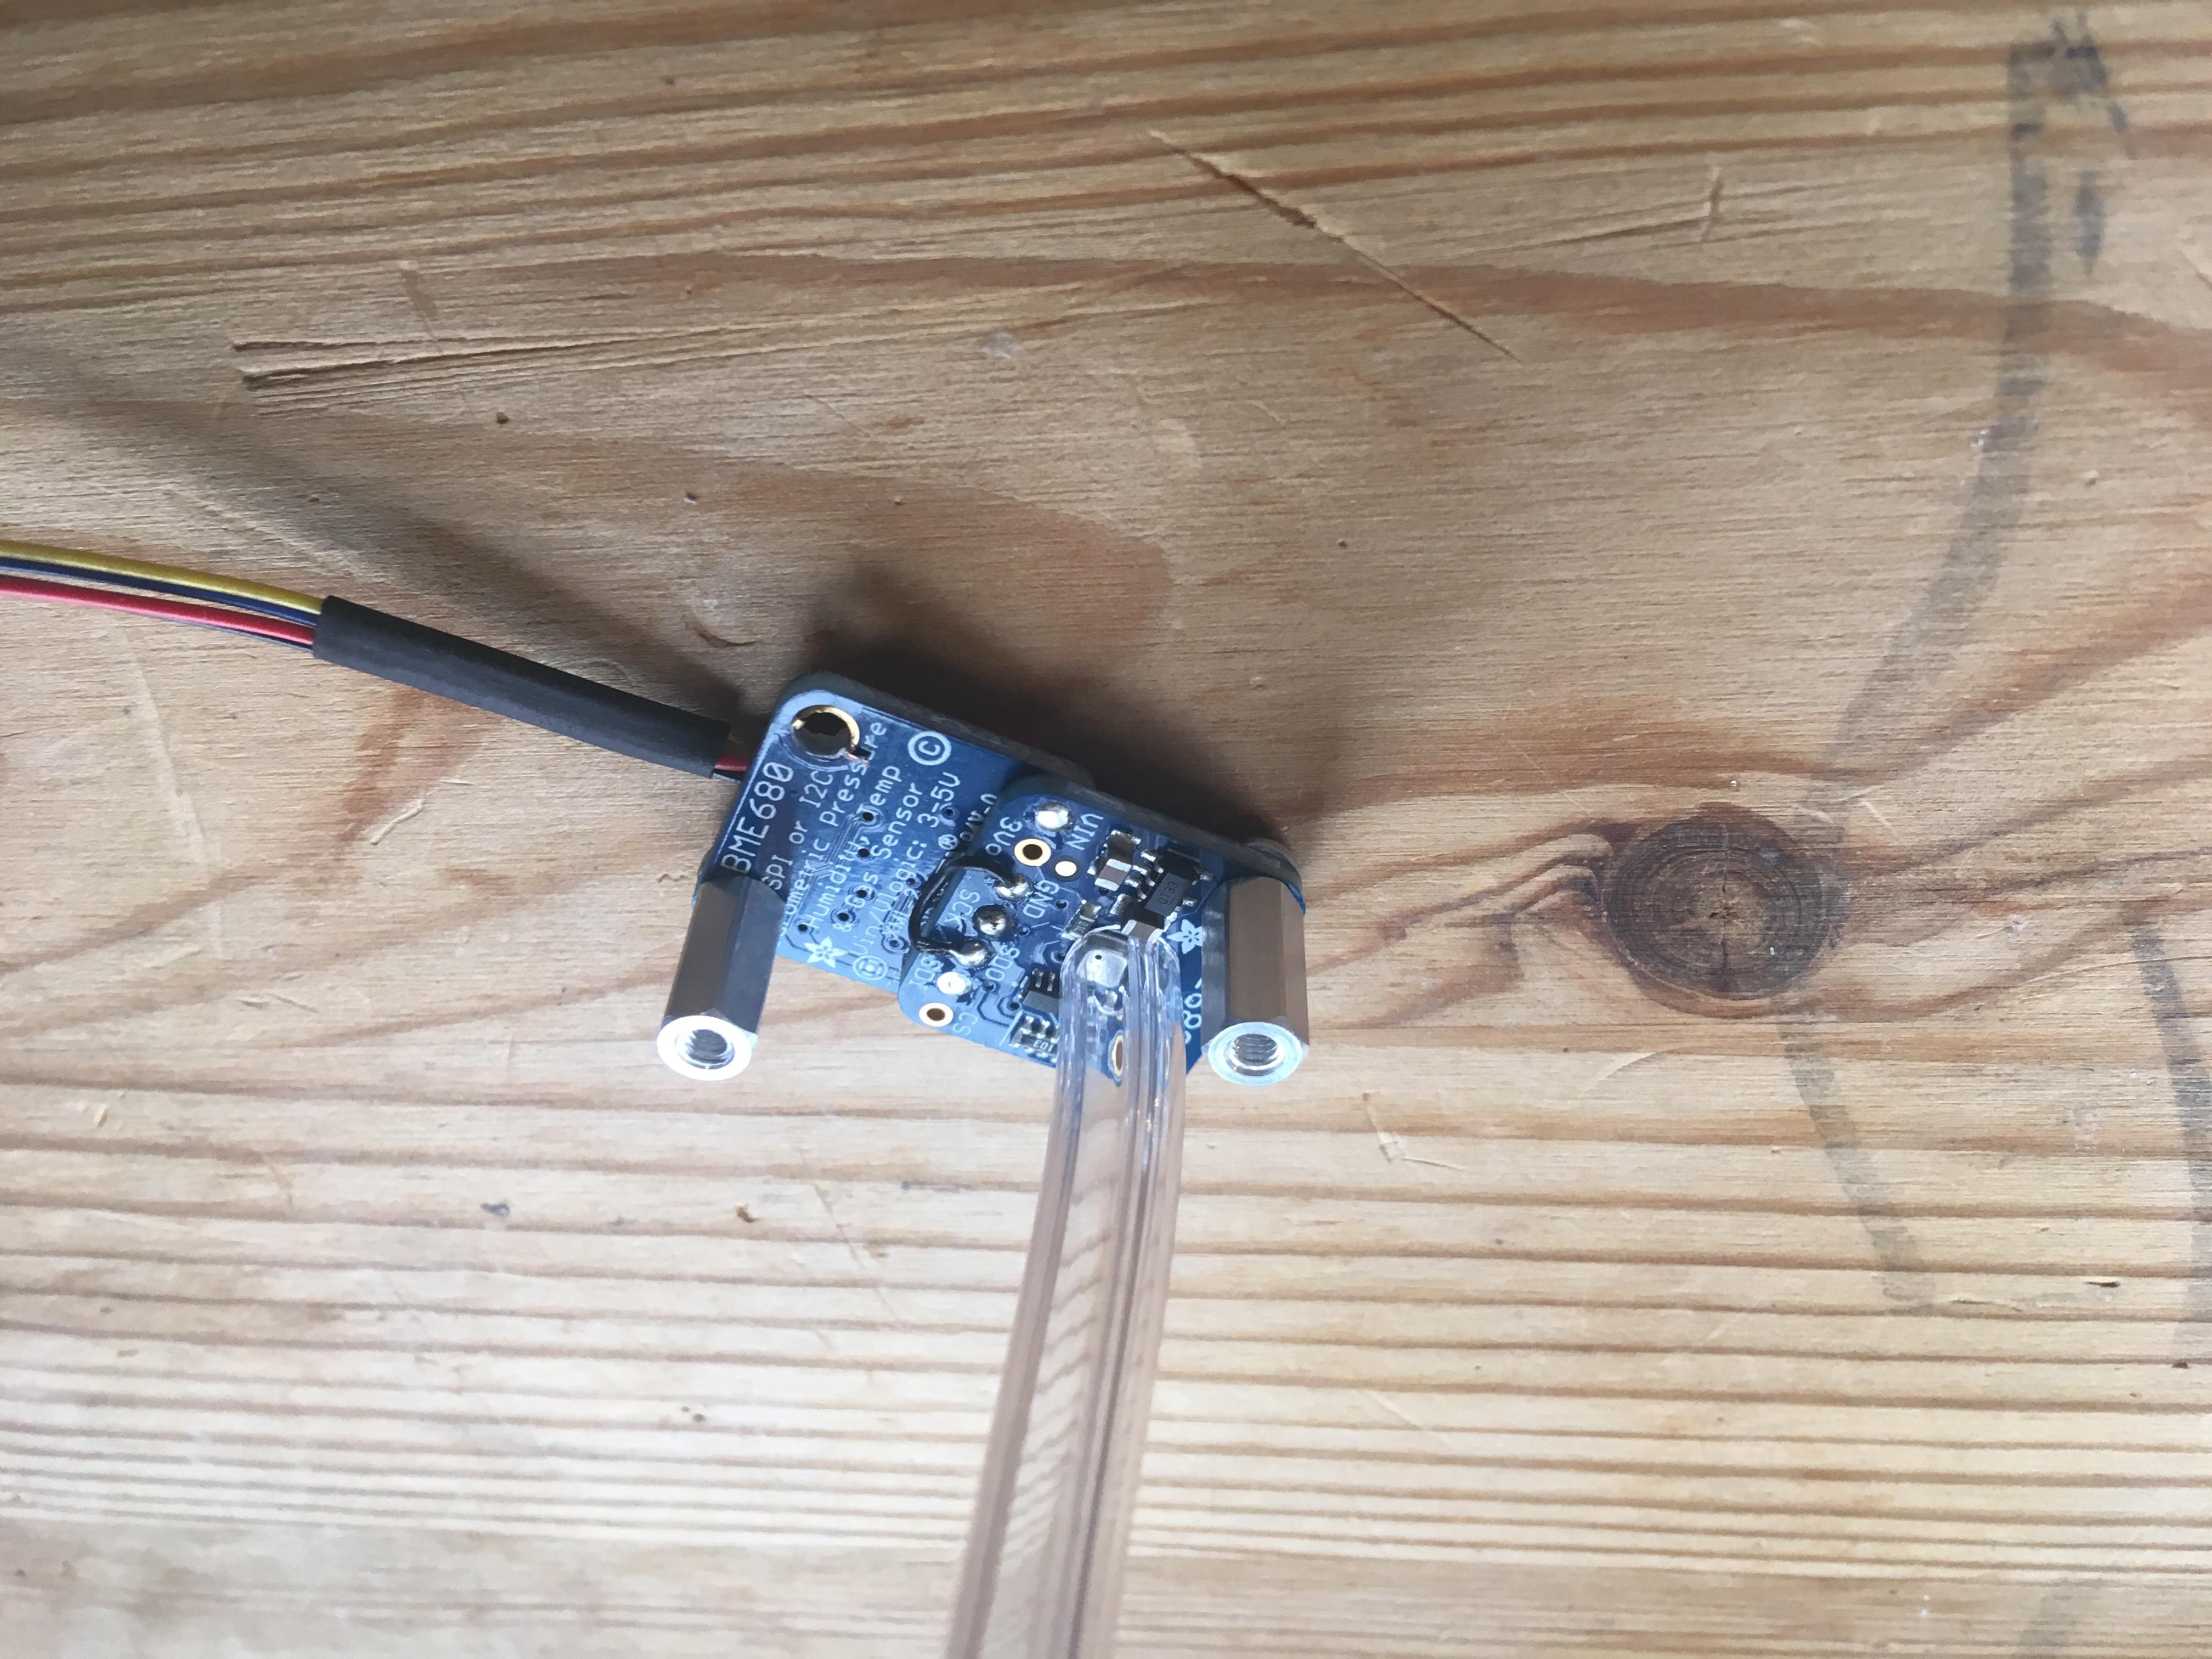
\includegraphics[width=0.6\textwidth, angle =90 ]{images/hotglue.JPG}
\caption{Standoffs installed on pressure sensor assembly and oxygen hose prepared for gluing.}
\label{fig:bme_glue}
\end{figure}

\item
Install pressure sensor assembly. Refer to figure \ref{fig:bmeinbox} on page \pageref{fig:bmeinbox}.
\begin{enumerate}[label=5.2.\arabic*]
\item
Add two standoffs to opposite corners of the pressure sensor assembly
\item
These should correspond to the mounting holes you drilled in the enclosure
\item
Thread the bare end of the oxygen hose through its hole in the enclose from the inside until the sensor assembly is pressed against the wall of the  enclosure
\item
Attach the standoffs into the enclosure from the outside using two machine screws
\end{enumerate}
\begin{figure}[H]
\centering
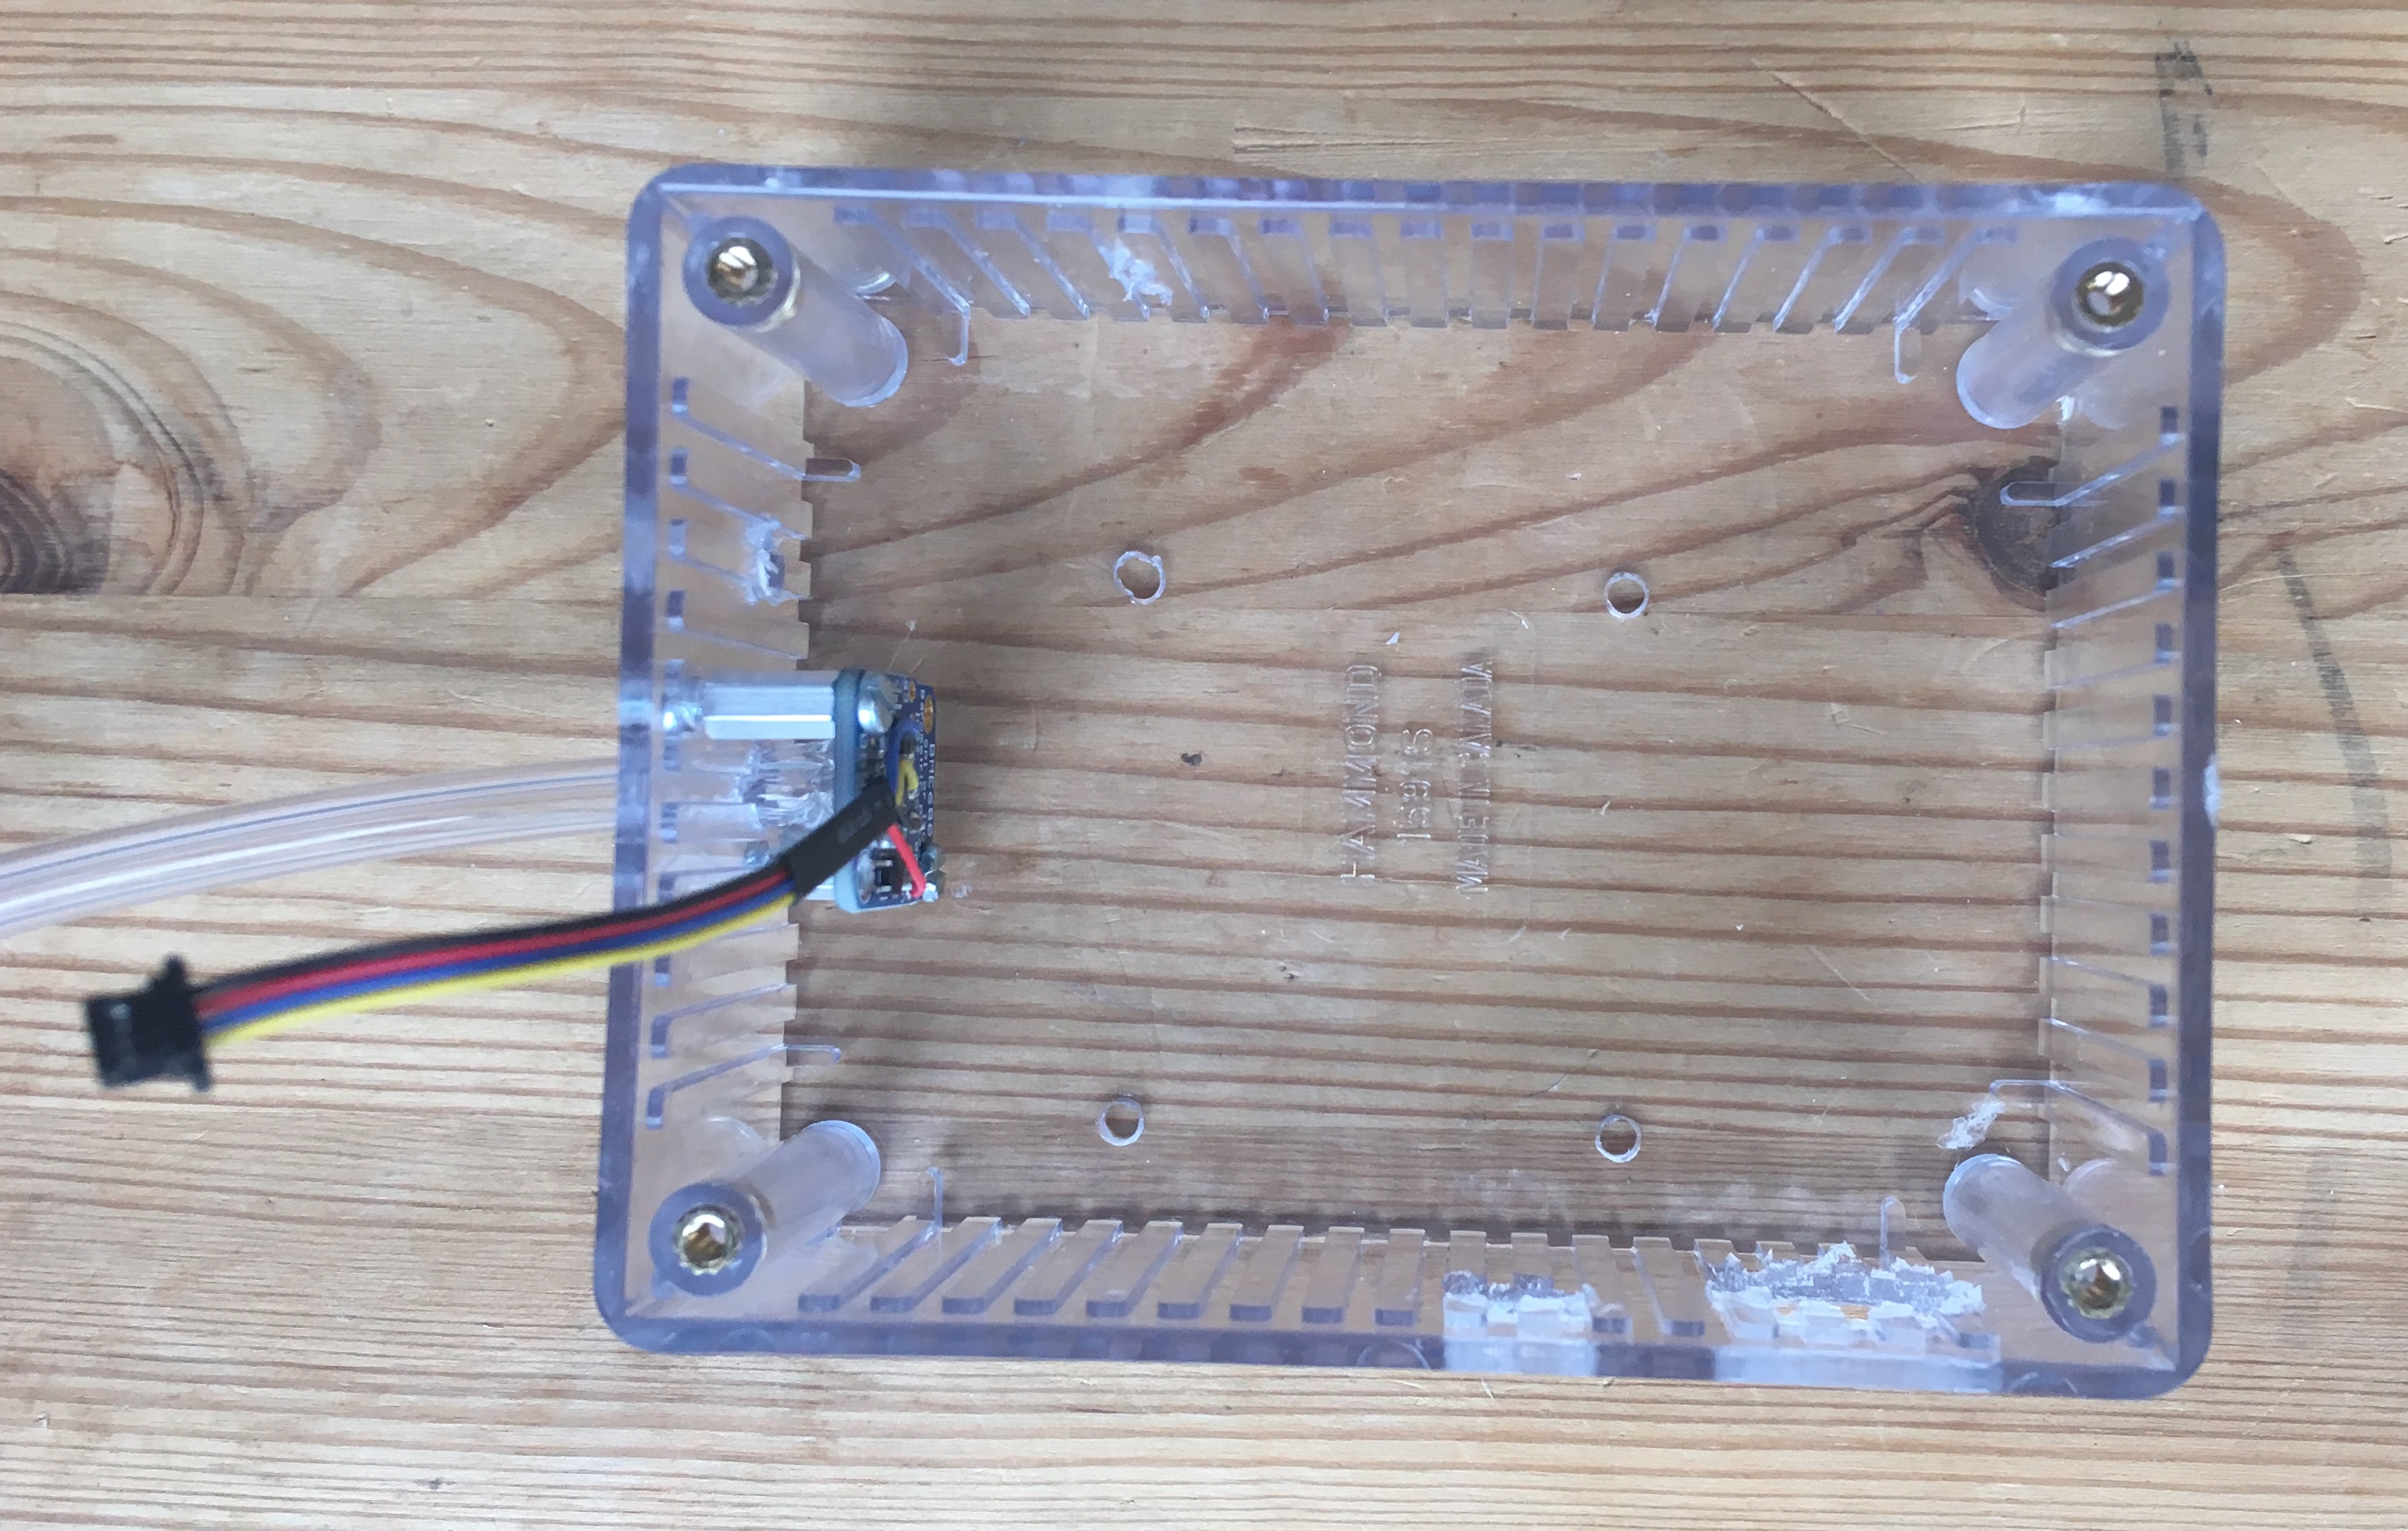
\includegraphics[width=0.8\textwidth]{images/bmeinbox.JPG}
\caption{Pressure sensor assembly installed in enclosure.}
\label{fig:bmeinbox}
\end{figure}
\item
Zip tie sensor cable to enclosure. Refer to figure \ref{fig:ziptie} on page \pageref{fig:ziptie}.
\begin{enumerate}[label=5.3.\arabic*]
\item
Thread the small zip tie through the two mounting holes in the enclosure
\item
Push the qwiic connector end of the flow sensor cable through its hole in the enclosure. It's a tight fit.
\item
Zip tie the cable to the side of the enclosure making sure that the jacket of the USB cable is engaged by the zip tie
\end{enumerate}
\begin{figure}[H]
\centering
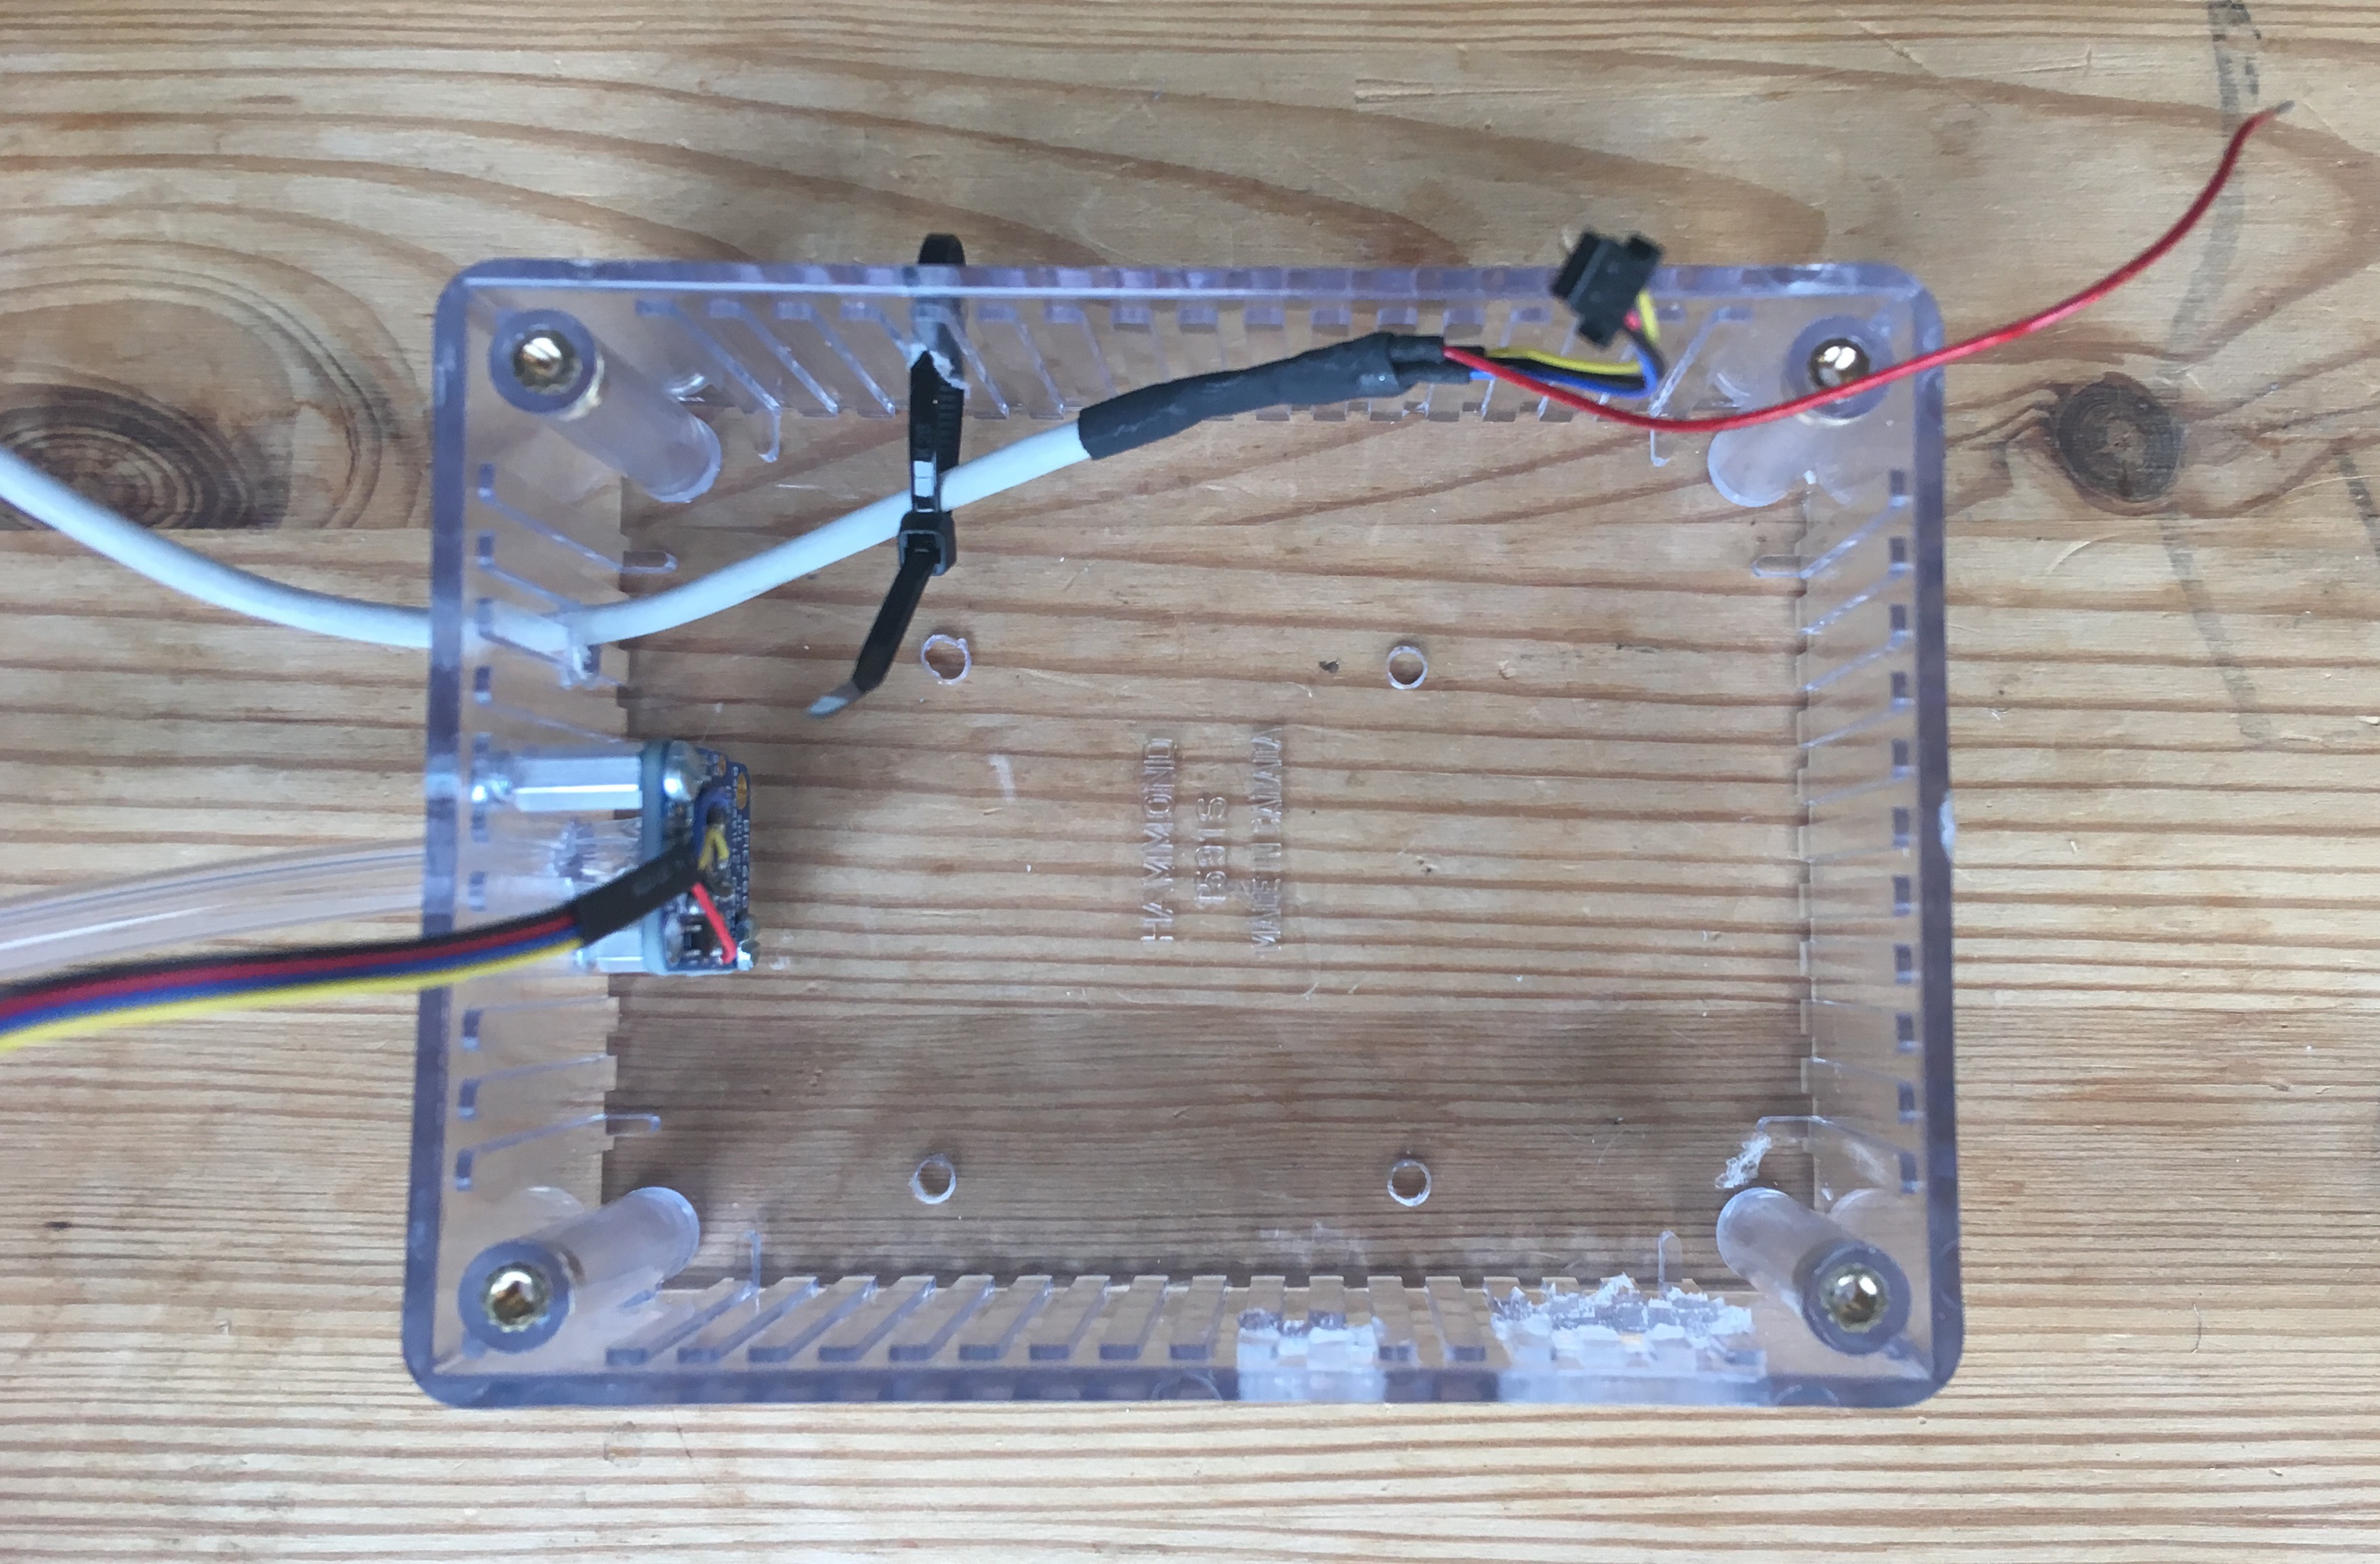
\includegraphics[width=0.8\textwidth]{images/ziptie.JPG}
\caption{Flow sensor cable with strain relief.}
\label{fig:ziptie}
\end{figure}


\item
Install ethernet shield and processor and add final touches.  Refer to figure \ref{fig:ziptie} on page \pageref{fig:ziptie}.
\begin{enumerate}[label=5.4.\arabic*]
\item
Attach standoffs to the four corners of the ethernet shield
\item
Screw the standoffs into the enclosure from the bottom
\item
Place the ESP32, OLED wing, and Qwiic shield on top of the ethernet shield as depicted in the diagram
\item
Plug the flow sensor and pressure sensor assembly into the qwiic shield
\item
Add a small piece of electrical tape every 5 inches attaching the oxygen tubing and flow sensor cable
\item
Wrap a piece of electrical tape around the flow sensor covering the exposed pads of the flow sensor
\item
Add identification card on the next page card to enclosure.
\begin{figure}[H]
\centering
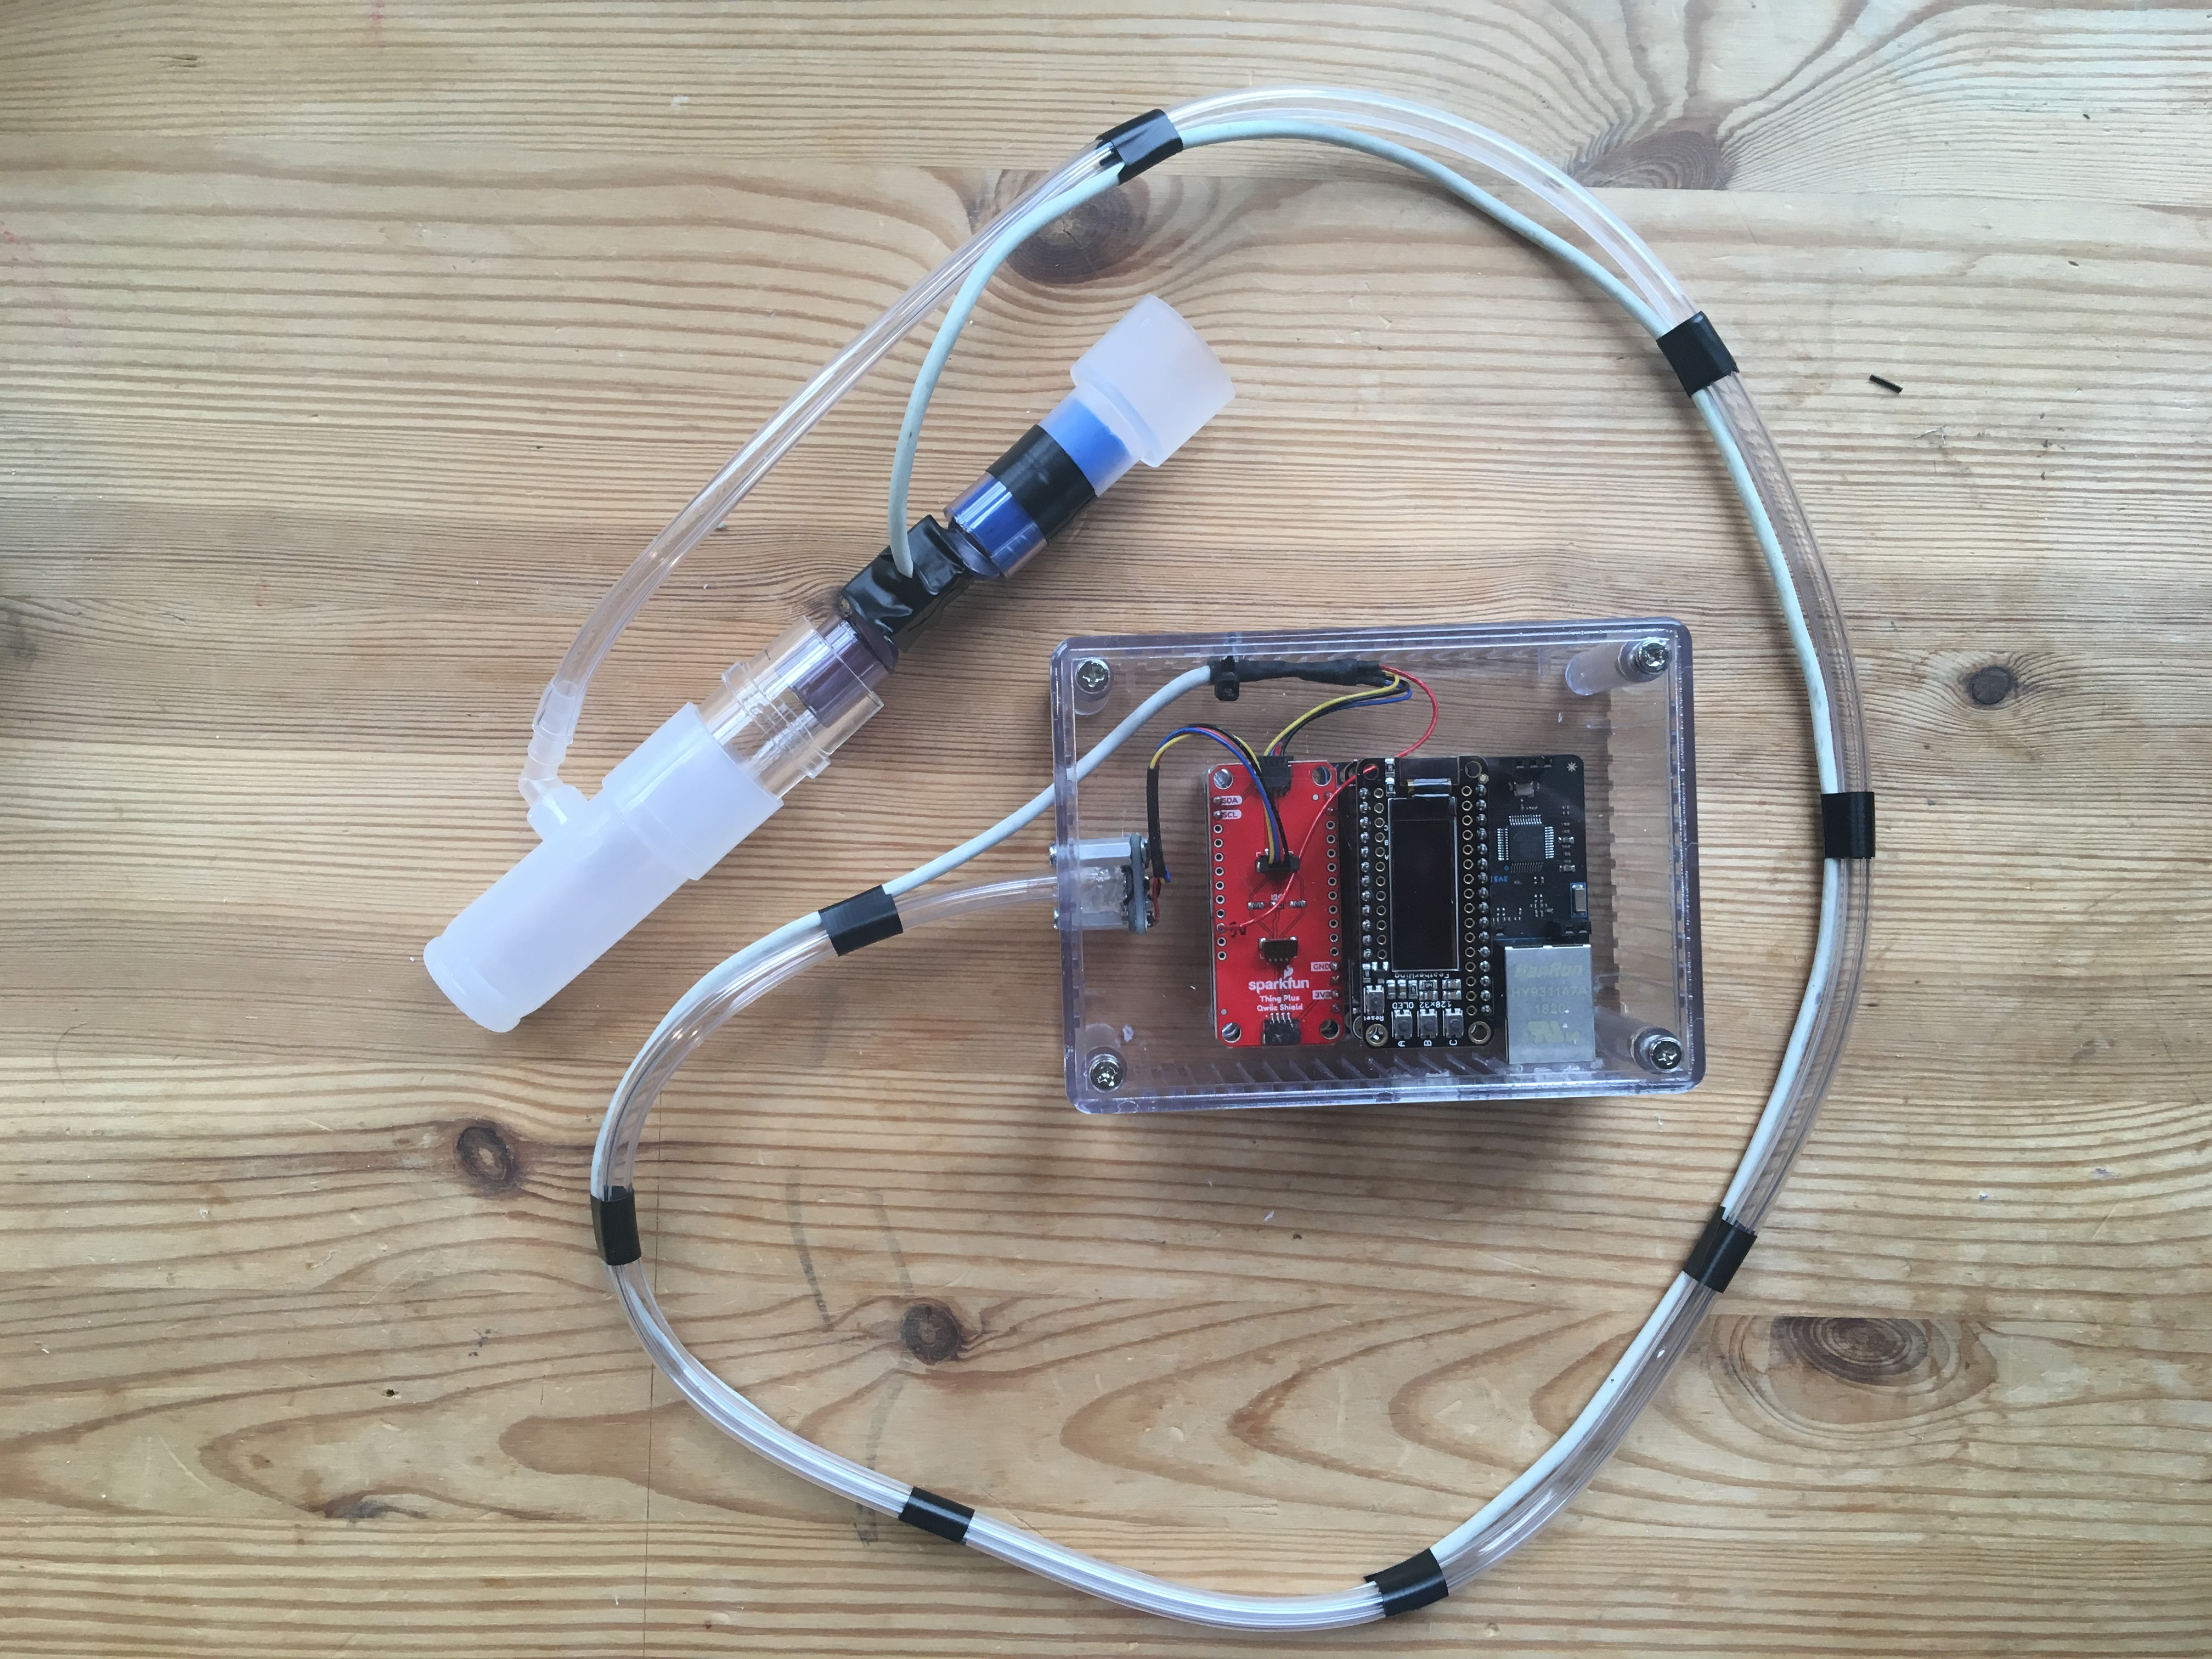
\includegraphics[width=\textwidth]{images/final_assembly_with_tape.JPG}
\caption{Final assembly.}
\label{fig:final}
\end{figure}
%\begin{enumerate}[label=5.4.\arabic*]
\end{enumerate}
\end{enumerate}
\end{enumerate}

%-----------------------------------------------------------

\subsection{PCB Based VentMon (v0.3T)}


\begin{figure}[H]
\centering
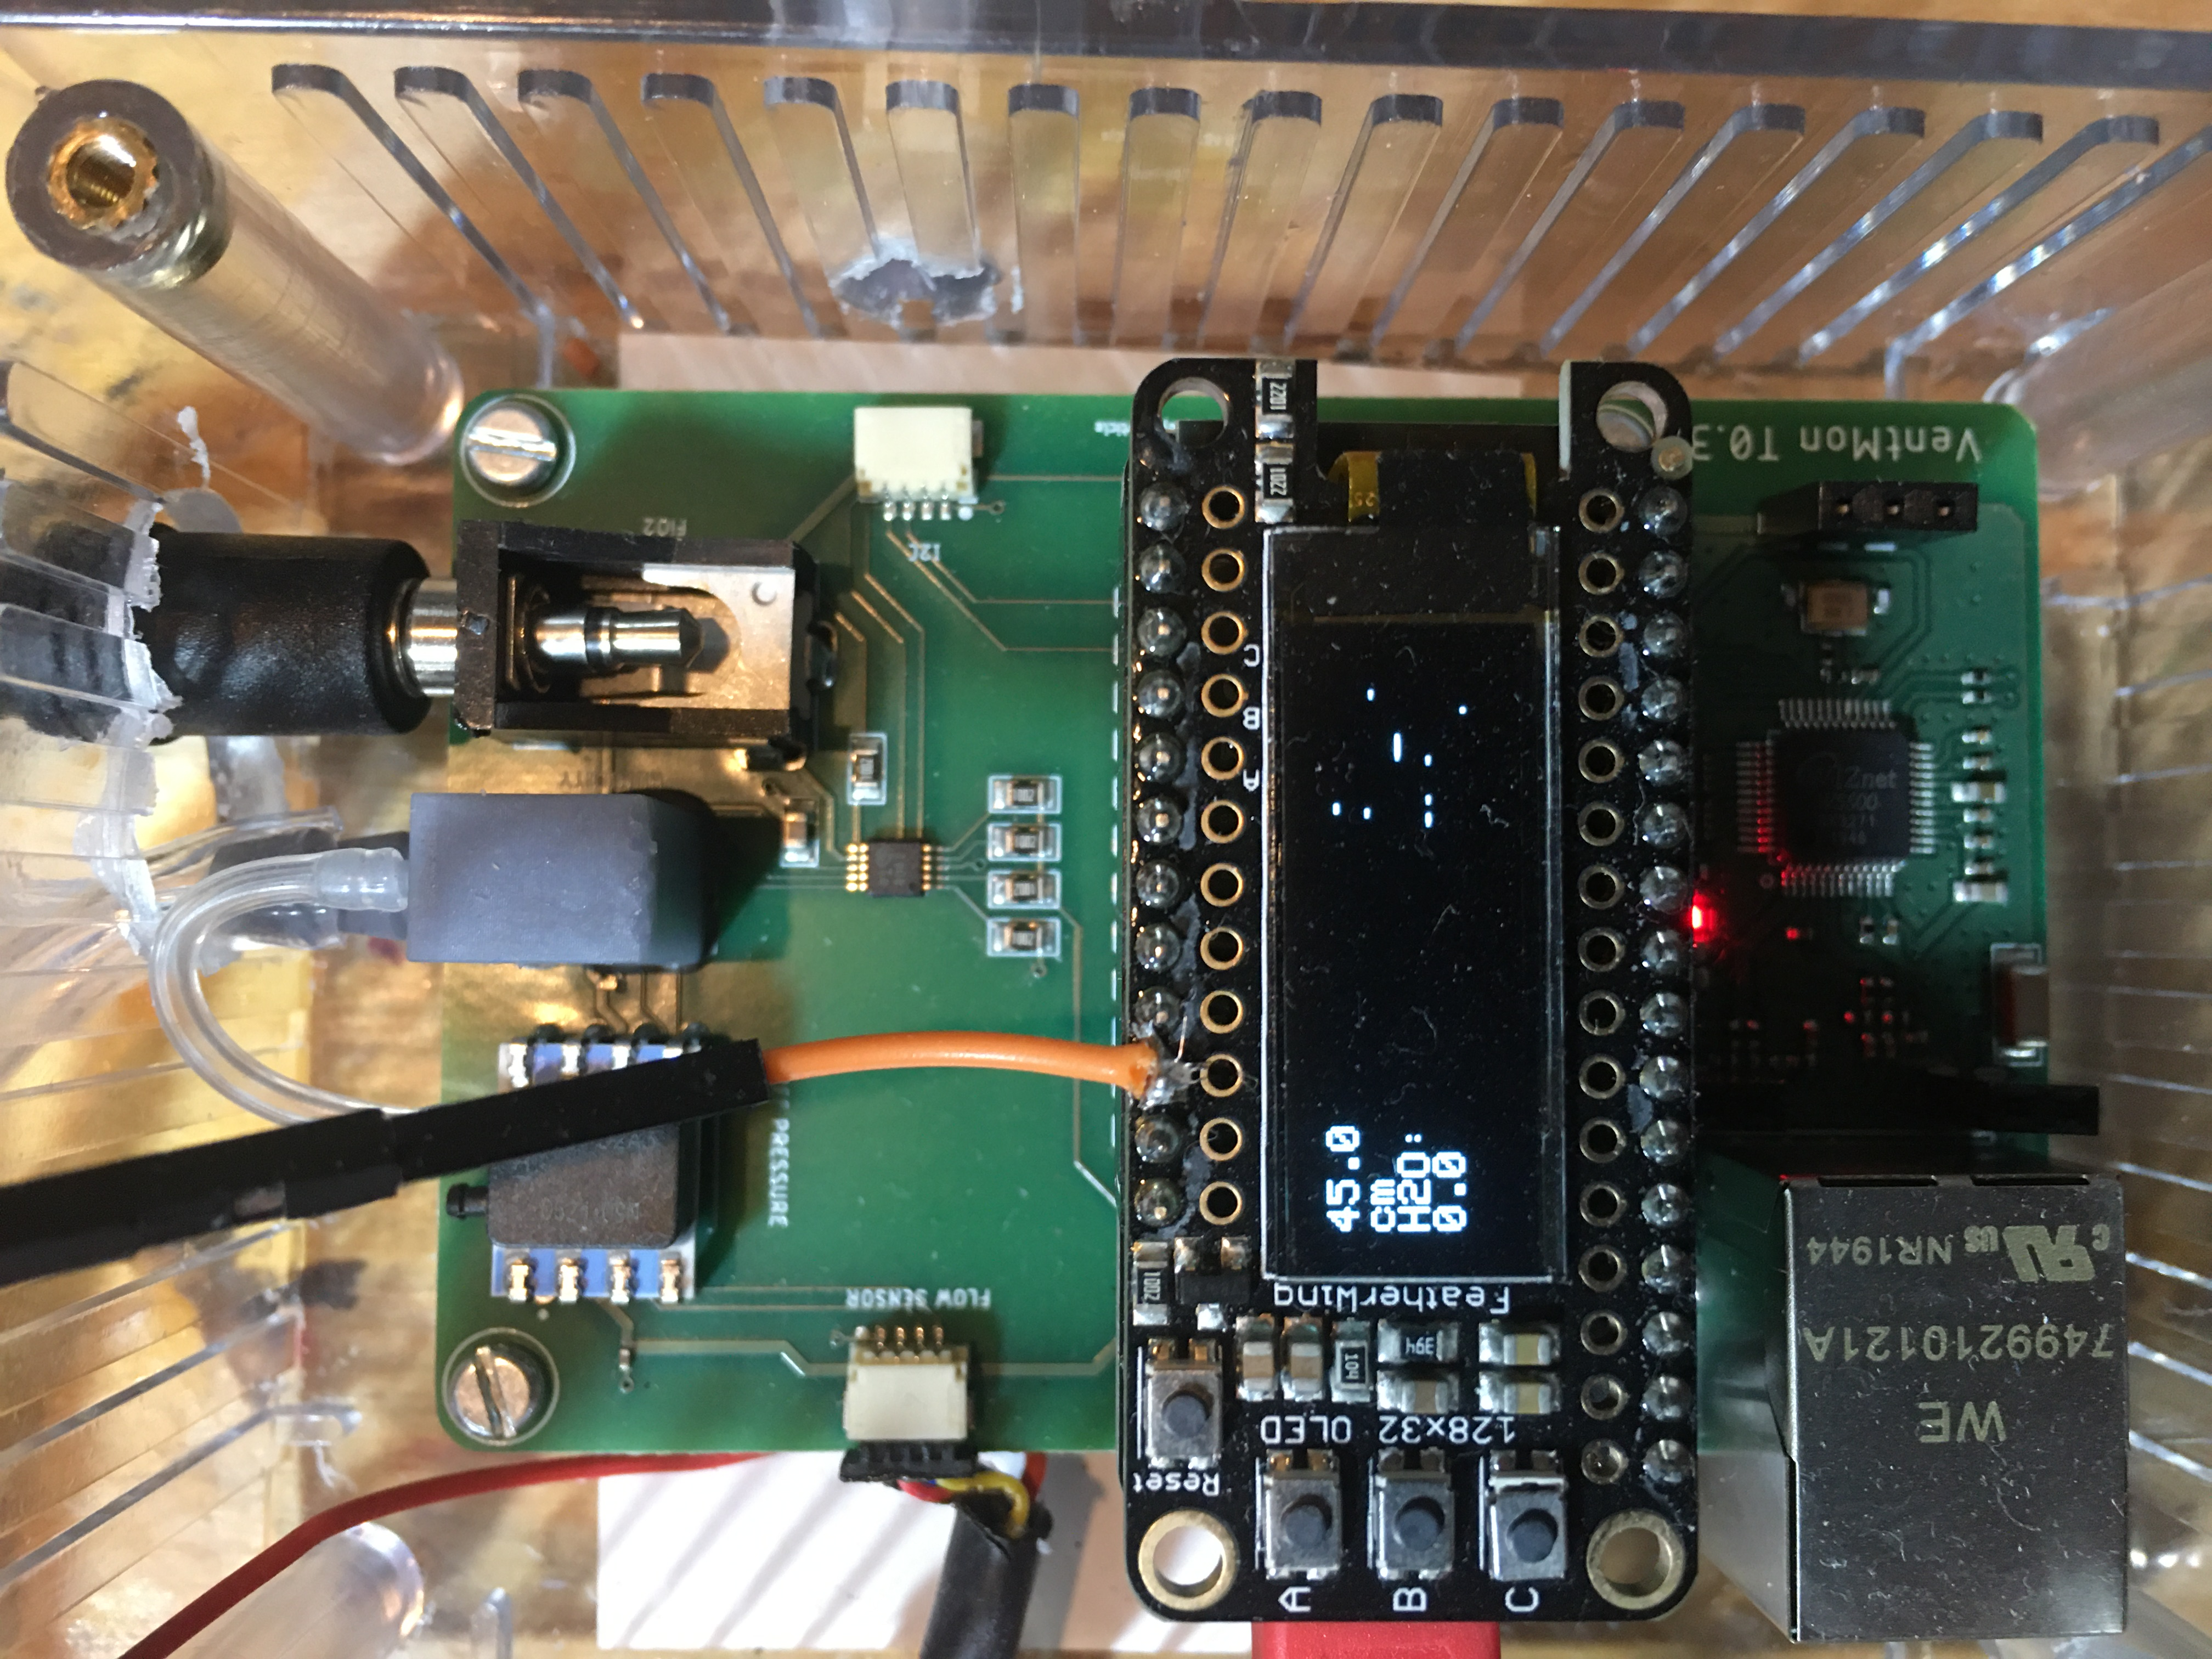
\includegraphics[width=\textwidth]{images/PCBVentMon.JPG}
\caption{Final assembly of the PCB version}
\label{fig:finalPCB}
\end{figure}

This PCB-based v0.3T version of VentMon (see Figure \ref{fig:finalPCB}) requires two 3D printed parts---one encapsulated an on-board pressure sensor and one is an airway adaptor---as well as a PCB assembly. Before beginning the assembly process make sure that you have manufactured those parts.

\begin{enumerate}
\item
PCB Assembly

\begin{enumerate}[label=1.\arabic*]
\item Add standoffs to PCB
\begin{enumerate}[label=1.1.\arabic*]
\item take hardware and put it in the holes
\end{enumerate}

\item Mount sensor enclosure for BME280 pressure sensor
\begin{enumerate}[label=1.2.\arabic*]
\item Insert plastic part into mounting holes on PCB to check fit and alignment. The barb should face toward the outer edge of the PCB.
\item Apply epoxy glue to bottom edge and mounting pegs of plastic.
\item Insert plastic back into holes being careful not to get any glue on the sensor.
\item Allow 24 hours for epoxy glue to cure before attaching a hose to the barb.
\end{enumerate}


\end{enumerate}

\item
Enclosure

Follow assembly instructions in section \ref{itm:enclosure}.

\item
Flow Sensor Assembly

Follow assembly instructions in section \ref{itm:flow}.

\item
Oxygen Sensor Assembly

\begin{enumerate}[label=4.\arabic*]
\item
Screw the airflow flange on to the oxygen sensor
\item
Plug sensor into the blue airway adaptor piece
\item
Plug one end of mono audio cable into bottom of oxygen sensor
\item
Plug the other end into the audio connector on the PCB
\end{enumerate}

\item
  Final Assembly
  \begin{enumerate}[label=4.\arabic*]
  \item Connect Qwiic connector.
  \item Screw lid on.
    \item Optionally apply hot-melt glue to Qwiic cable connector where it enters the port.
    \end{enumerate}

\end{enumerate}

%----------------------------------------------------------

\section{Operation instructions}
%Provide detailed instructions for the safe and proper operation of the hardware.
%> Step-by-step operational instructions for operating the hardware.
%> Use visual instructions as necessary.
%> Highlight potential safety hazards.

\begin{figure}[H]
\centering
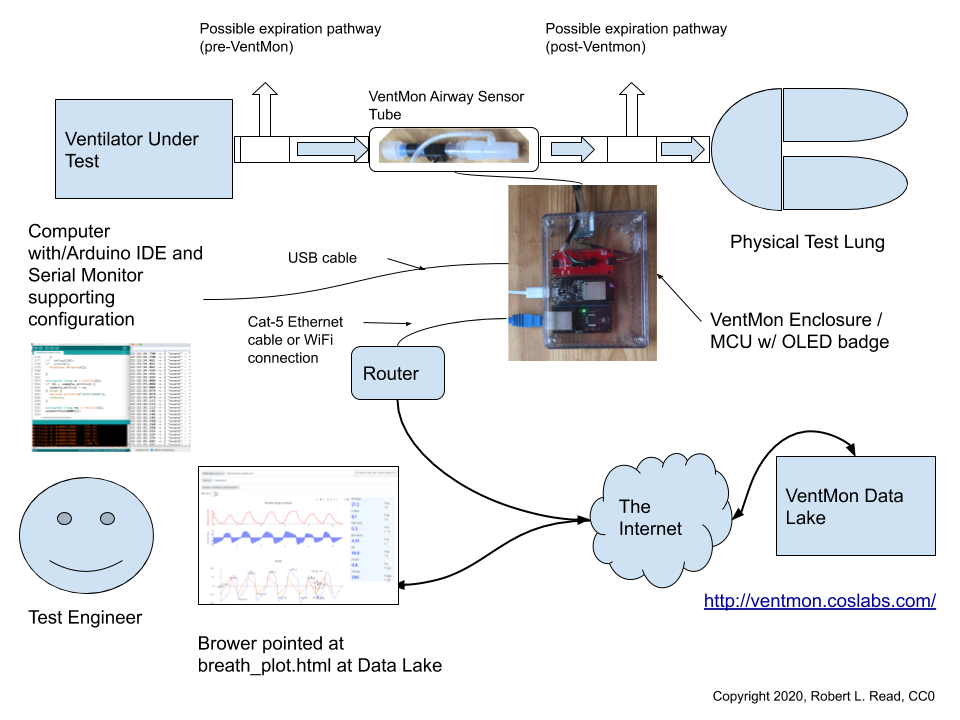
\includegraphics[width=\textwidth]{images/VentMonOverallArchitecture.png}
\caption{Ventilator Test Usage}
\label{fig:vtestusage}
\end{figure}


\subsection{VentMon v0.3T}

{\em The VentMon v0.3T is not meant to be used on human patients. }
The purpose of the VentMon is to measure, log, validate and verify the performance of rapidly manufactured ventilators, PAPRs, BPAP, and CPAP machines. The basic usage is to plug the VentMon 22mm airway in between a respiration assistance device being tested (such as a pandemic ventilator or CPAP machine) and a simple physical test lung which models compliance and resistance of the human lung (see Figure \ref{fig:vtestusage}). The VentMon then provides approximately the functionality of a {\em breathing simulator}, without being able to model the patient triggering a breath spontaneously.

There are four ways to get data from the VentMon of varying quality and convenience with the firmware at the time of this writing.
\begin{enumerate}
\item After startup, the VentMon will begin displaying a real-time pressure graph on its small OLED screen, with a scale of 40 cmH$_2$O. This display is too small for testing performance, but is a nice check that the breathing circuit is in place and functioning. You can ``smoke test'' this by breathing into the VentMon and plugging one end with your hand.
\item The VentMon spews a LOT of data out on the serial port in the PIRDS format. Using the serial monitor built into the Arduino IDE, you can visually inspect this data. The volume of the data makes this a cumbersome. You are free to write a serial-port reader of your own for programmatic interpretation.
\item At startup, by default configuration (it can be enabled or disabled), the VentMon tries to see if their is a cable connected to the Ethernet RJ45 jack. Plug the other end of the cable into your router. If found and enabled, the VentMon will begin sending PIRDS\cite{PIRDS} data to the logger at \url{ventmon.coslabs.com}\cite{PIRDSlogger}. Your data can be viewed in real time by pointing a browser at the URL. Your IP address will appear near the top of the list with other recent or current users; by clicking on ``Breath Plot'' you will be able to see a complete clinical display.
\item Similarly at startup, the VentMon will attempt to establish a WiFi connection. Using the WiFi connection will transmit exactly the same PIRDS data the logger at \url{ventmon.coslabs.com} and can be used in precisely  the same way. However, the VentMon has to know a valid SSID and password to make the WiFi connection. This is configured via the Arduino serial monitor by sending a ``c'' character (for configure) to the VentMon. It will then pause operation for 10 seconds and give instructions for entering the SSID and password. In this same configuration you can enable or disable the WiFi and the Ethernet connection if you choose. These settings are stored in the EEPROM, and survive a loss of power.
\end{enumerate}

Pressing the ``C'' button on the VentMon OLED badge sends a special signal to the PIRDS logger to ``rotate the log'' from this IP address. At the public data lake the current file will be copied to a file which a date and timestamp.

\subsection{VentMon COTS Version}

A practitioner who makes their own version of the VentMon from commercial off-the-shelf parts without ordering a PCB will likely understand how to install
and modify the firmware. The VentMon v0.2T\cite{VentMon02} version is tagged specifically for this hardware release. The usage will likely be the same, though at the time of this writing some features
may not be available in the software they are using, such as WiFi configuration.

\section{Validation and characterization}

%Demonstrate the operation of the hardware and characterize its performance over relevant critical metrics
%> Demonstrate the use of the hardware for a relevant use case.
%> If possible, characterize performance of the hardware over operational parameters.
%> Create a bulleted list that describes the capabilities (and limitations) of the hardware. For example consider descriptions of load, operation time, spin speed, coefficient of variation, accuracy, precision and etc.

The primary use of the VentMon is to develop to and verify that rapidly manufactured ventilator meets requires specification, such as those published by the UK MHRA\cite{mhra2020specification}.

It is easy to have confidence in the basic dynamic function of the VentMon by simply breathing through it into a plastic test lung. Figure \ref{fig:ventdisplay} is a screenshot of VentDisplay rendering data from the VentMon with a human (RLR) breathing normally into a plastic test lung for 10 seconds. Although the VentDisplay and VentMon can be used independently, VentDisplay demonstrates what VentMon collects. The top trace is a pressure trace. The next shows flow. These curves are generated from samples published into the public data lake. VentMon produces pressure and flow graphs at about 25 samples per seconds which is fast compared to the physiological process of breathing. One can easily see that flow and pressure dynamically match the breath or changes in the mechanical ventilation, or even changes induces by changes in the resistance of compliance of the test lung.

The bottom trace on the display is the ``event'' curve which shows a number of computed values and events published from the VentMon, such as the humidity, FiO$_2$, and temperature. Additionally, the beginning and ending of each breath is detected, and total volume of the breath computed by integrating the flow.


\begin{figure}[H]
\centering
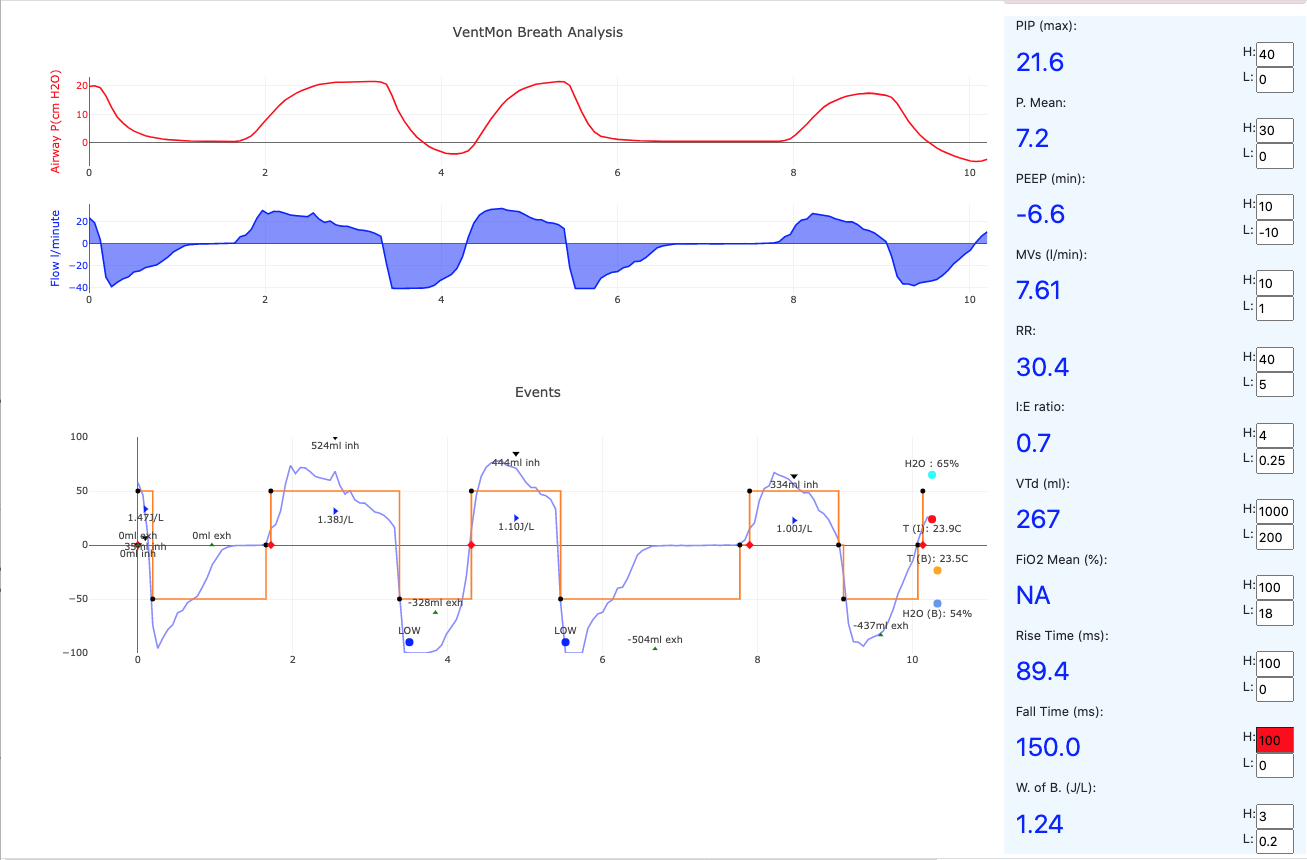
\includegraphics[width=\textwidth]{images/VentDisplayExample.png}
\caption{VentDisplay Data Display}
\label{fig:ventdisplay}
\end{figure}

These calculations allows us to present the numbers on the right side of the display, which are typical metric found on a commercial ventilator. Computation of these values allows a would-be ventilator's performance to be verified and characterized against a repeatable and relevant standard. Features such as rise and fall time (at the bottom on the right) are particularly important. However, the most basic function is to dynamically report the respiration rate, peak pressure, minimum pressure, tidal volume and minute volume, and I:E ratio. In addition to the standard metrics, our software also measures pressure rise time which we have argued is an under-appreciated performance characteristic of rapidly manufactured emergency ventilators\cite{schulz2020importance}.

This software has been shown to be valuable, although it is dependent on accurate software decisions about
the beginning and the ending of a breath, which can be subtle in some situations. The reliability of the data is inherently tied to the accuracy and precision of the device producing data for VentDisplay. VentMon is unique in this regard as the flow, differential pressure, and oxygen sensors used in the design require no calibration. After independent testing of each component, the VentMon team found that oxygen sensing and flow measurements using ther device were accurate within 10\% and X\% respectively.		
%flow and oxygen measurements are suitable for accurately measuring FiO$_2$ mixing in mechanical ventilation. 

The Public Invention Respiration Data Standard format \cite{PIRDS}, is the underlying method by which data is communicated from the VentMon device to VentDisplay. The standard was created to provide a repeatable way for multiple teams to cooperate. Using this standard and cloud-based software enables VentMon to support a distributed engineering team---often required by the COVID-19 social distancing measures. The VentDisplay software allows export of the JSON binding of the PIRDS data to allow other programs to process if it if desired. We believe these tools could someday allow us to support telemedicine as suggested by others \cite{rehm2018development}.

In fact we hope the VentMon will evolve into an open-source component that can be freely integrated into a pandemic ventilator or simply ``bolted on'' to be used to control ventilators or to monitor human patients. Although it can effectively test ventilation equipment today, before it can be recommended for use on patients, it will require regulatory approval, such as FDA approval. Before that can happens, the VentMon must progress beyond a number of limitations:
\begin{enumerate}
\item The current device is not autoclavable or easy to sanitize. Use on a human patient would therefore require it to be disposed of immediately.
\item Our software has not be subject to rigorous Quality Assurance (QA) and Risk Analysis (RA) as the FDA would request. We have argued\cite{ecosystem} for an ecosystem in which design teams such as Public Invention produce extensive documentation including  QA/RA documentation to be reused by firms that become medical device manufactures incorporating open-source designs.
\item The mechanical design of the VentMon will require additional alteration to make it robust enough for use in a clinical setting.
\item The current data lake and software allow data  logging over days or weeks. To enable longitudinal study of ventilator reliability we would like to create software that allows this data to be analyzed or accessed across long periods of time.
\end{enumerate}



\section{Acknowledgements}
% [List here those individuals who provided help during the research (e.g., providing language help, writing assistance or proof reading the article, etc.).] Please also identify who provided financial support for the conduct of the research and/or preparation of the article and to briefly describe the role of the sponsor(s), if any, in study design; in the collection, analysis and interpretation of data; in the writing of the report; and in the decision to submit the article for publication. If the funding source(s) had no such involvement then this should be stated.}

Robert L. Read: Conceptualization, Methodology, Software, Writing - Original Draft, Supervision.
Lauria Clarke: Software, Hardware, Investigation, Writing - Review and Editing.
Geoff Mulligan: Conecptualiztion, Software.

Robert L. Read conceived of and wrote most of the firmware for the VentMon.
Geoff Mulligan created the initial cloud-based IoT approach which became the PIRDS-logger.
Lauria Clarke did most of the hardware design, including the assembly instructions and
the printed circuit board based on an MIT-licensed Ethernet Feather Wing design
from Particle IoT\cite{particleefw}, and the SFM3X00 software repo for
encapsulating Sensirion flow sensors in the Arduino environment.
This paper was written by Robert L. Read and Lauria Clarke.

The Mozilla Open Source Software foundation gave Public Invention a grant that allowed us to develop the hardware and provide 20 VentMons to open source teams around the world free-of-charge, including paying shipping costs. Protocol Labs provided Public Invention a grant that has been used for web communication and conference costs.

We would like to thank early adopters of the VentMon on pandemic ventilator teams such as the ARMEE\cite{ARMEE}, PolyVent\cite{polyvent} and DIY-Beatmungsgerät.de\cite{beatmung} who gave us valuable bug reports and feedback.

Adafruit graciously continued to supply pandemic engineers and researchers even when their normal business was disrupted.

Student volunteers on the COVID19-vent-list project\cite{COVID19VENTLIST} helped to make the need for the VentMon clear by assessing over 100 pandemic ventilator teams.

\section{Declaration of interest}

None.
% a statement must be included even if there is no conflict of interest
% All authors must disclose any financial and personal relationships with other people or organizations that could inappropriately influence (bias) their work. Examples of potential conflicts of interest include employment, consultancies, stock ownership, honoraria, paid expert testimony, patent applications/registrations, and grants or other funding. Authors must disclose any interests in a summary declaration of interest statement in the manuscript file. If there are no interests to declare then please state this: 'Declarations of interest: none'. This summary statement will be ultimately published if the article is accepted. More information.}



% This work touched no humans or animals, I belive this section can be ommmited entirely.
% \section{Human and animal rights}



% \section*{References}
%> Include at least one reference, to the original publication of the hardware you customized.
%> Include other references as required. Include references to put your device in context in the literature. For more information on the reference format in HardwareX please see the Guide for Authors at: https://www.elsevier.com/journals/hardwarex/2468-0672/guide-for-authors




\printbibliography

\end{document}

%> Author manuscript checklist
%> ●	HardwareX is a journal dedicated to the exhaustive and fully open source communication of advances in scientific infrastructure. Upon submission the author declares that all information necessary to reproduce the subject of the submission (e.g. bill of materials, build instructions, calibration procedures, source files, code, and safety considerations) is communicated in full and is accessible for use under an open source license.
%> ●	Is the subject of the submission under an open source license - as defined by the Open Source Hardware definition?
%> ●	Can the hardware be reproduced with the details provided in the submission?
%> ●	Are all relevant design files available on Mendeley Data, the Open Science Framework, or Zenodo repositories, described in the Summary of Design Files document, and clearly documented? (e.g. descriptive file names, commented code, labeled images, etc.)
%>      ○	If in the Open Science Framework, the repository has be registered? Instructions
%>      ○	If in Zenodo, the repository is open access and is published? Instructions
%>      ○	If in Mendeley Data, the repository is published or the sharable link was included in the additional information of the Editorial Submission interface? Instructions
%> ●	Are visual instructions used when necessary?
%> ●	Is the utility of the hardware to the scientific community?
%> ●	Is the performance of the hardware adequately demonstrated and characterized?
%> ●	Are all potential safety concerns addressed?
%> ●	For more information on the article template consult the Guide to Authors.}


% Notes:
% Potential reviewers: Michelle Mellenthin, Eric Schulz, Angela Forgues
